\section{Model opstilling}
%%%%%%%%%%%% MID WAY AGENDA %%%%%%%%%%%%%%
\begin{frame}<beamer>
\frametitle{Daniel Bähner Andersen}
\tableofcontents[currentsection]
\end{frame}
%%%%%%%%%%%% MID WAY AGENDA %%%%%%%%%%%%%%


\subsection{Trolley- og pendulmodel}
\begin{frame}{Model opstilling}{Trolley- og pendulmodel}
  \begin{minipage}[t]{0.50\linewidth}
    \begin{itemize}
      	\item<1->[] {
              \begin{figure}[H]
              \centering
              \scalebox{0.75}{\input{Billeder/Daniel/mechanicalSystem.ralf}}
              \end{figure}}
        \item<3->[] {
     		\begin{equation*}
				m_t \ddot{x} = F_a - F_{sx_p} - F_{Bt} = F_a - F_s \cdot \sin(\theta) - B_t\dot{x}
			\end{equation*}}      
    \end{itemize}           
  \end{minipage}
  \begin{minipage}[t]{0.45\linewidth}
\bigskip
\bigskip 
\bigskip
	\begin{itemize}
    	\item<2->[] Fritlegeme diagram for trolley  
	\end{itemize}    
\medskip 
    \begin{itemize}            
	\item<2->[] {
              \begin{figure}[H]
              \centering
              \scalebox{0.75}{\input{Billeder/Daniel/FBDtrolley.ralf}}
              \end{figure}}	     	
    \end{itemize}           
  \end{minipage}
\end{frame} 
%%%%%%%%%%%%%%%%

\begin{frame}{Model opstilling}{Trolley- og pendulmodel}
  \begin{minipage}[t]{0.50\linewidth}
    \begin{itemize}
      	\item<1->[] {
              \begin{figure}[H]
              \centering
              \scalebox{0.75}{\input{Billeder/Daniel/mechanicalSystem.ralf}}
              \end{figure}}
        \item<3->[] {
     		\begin{equation*}
				m_L \ddot{x_L} = m_L(\ddot{x} - \ddot{x_p}) =  F_{sx_p} + F_{Bx_p} = F_s \cdot \sin(\theta) + \frac{1}{L} B_p \dot{\theta} \cos(\theta)
			\end{equation*}} 
		\item<4->[] {
     		\begin{equation*}
				x_p = \sin(\theta) \cdot L \Rightarrow \ddot{x_p} = -\sin(\theta)\cdot \dot{\theta}^2 \cdot L + \cos(\theta)\cdot \ddot{\theta} \cdot L
			\end{equation*}}  	     
    \end{itemize}           
  \end{minipage}
  \begin{minipage}[t]{0.45\linewidth}
\bigskip
\bigskip 
\bigskip
	\begin{itemize}
    	\item<2->[] Fritlegeme diagram for pendulet i x-aksen  
	\end{itemize}    
\medskip 
    \begin{itemize}            
	\item<2->[] {
              \begin{figure}[H]
              \centering
              \scalebox{0.75}{\input{Billeder/Daniel/FBDPenX.ralf}}
              \end{figure}}	     	
    \end{itemize}           
  \end{minipage}
\end{frame} 
%%%%%%%%%%%%%%%%

\begin{frame}{Model opstilling}{Trolley- og pendulmodel}
  \begin{minipage}[t]{0.50\linewidth}
    \begin{itemize}
      	\item<1->[] {
              \begin{figure}[H]
              \centering
              \scalebox{0.75}{\input{Billeder/Daniel/mechanicalSystem.ralf}}
              \end{figure}}
        \item<3->[] {
     		\begin{equation*}
				m_L \ddot{y} =  F_{By_p} + F_g - F_{sy_p}  = \frac{1}{L} B_p \dot{\theta} \sin(\theta) + F_g - F_s \cdot \cos(\theta)
			\end{equation*}}
		\item<4->[] {
     		\begin{equation*}
				y = \cos(\theta) \cdot L \Rightarrow \ddot{y} = -\cos(\theta) \cdot \dot{\theta}^2 \cdot L - \sin(\theta) \cdot \ddot{\theta} \cdot L
			\end{equation*}}  	      
    \end{itemize}           
  \end{minipage}
  \begin{minipage}[t]{0.45\linewidth}
\bigskip
\bigskip 
\bigskip
	\begin{itemize}
    	\item<2->[] Fritlegeme diagram for pendulet i y-aksen  
	\end{itemize}    
\medskip 
    \begin{itemize}            
	\item<2->[] {
              \begin{figure}[H]
              \centering
              \scalebox{0.75}{\input{Billeder/Daniel/FBDPenY.ralf}}
              \end{figure}}	     	
    \end{itemize}           
  \end{minipage}
\end{frame} 
%%%%%%%%%%%%%%%%
% Resulterende modeller
%%%%%%%%%%%%%%%%

\begin{frame}{Model opstilling}{Trolley- og pendulmodel}
    \begin{itemize}
      	\item<1-> Overføringsfunktioner 
      	\begin{itemize}
      		\item<2-> Lineariseret 
      		\item<2-> Laplace tranformeret  
      	\end{itemize}	       
    \end{itemize}  
\bigskip
\bigskip             
  \begin{minipage}[t]{0.3\linewidth} 
    \begin{itemize}            
	\item<3->[] {\begin{equation*}
             		\frac{X(s)}{F_a(s)}   
                \end{equation*}}	
    \end{itemize}           
  \end{minipage}
  \begin{minipage}[t]{0.3\linewidth} 
    \begin{itemize}            
	\item<4->[] {\begin{equation*}
             		\frac{\Theta(s)}{F_a(s)} 
                \end{equation*}}	
    \end{itemize}           
  \end{minipage}
  \begin{minipage}[t]{0.3\linewidth} 
    \begin{itemize}            
	\item<5->[] {\begin{equation*}
             		\frac{X_L(s)}{F_a(s)}  
                \end{equation*}}	
    \end{itemize}           
  \end{minipage}

%%%%%%%%%%%%%%%%

\end{frame}
\begin{frame}{Model opstilling}{Trolley- og pendulmodel}
  \begin{minipage}[t]{0.48\linewidth}
    \begin{itemize}
      	\item<1->[] {
              \begin{figure}[H]
              \centering
              % This file was created by matlab2tikz.
%
%The latest updates can be retrieved from
%  http://www.mathworks.com/matlabcentral/fileexchange/22022-matlab2tikz-matlab2tikz
%where you can also make suggestions and rate matlab2tikz.
%
\definecolor{mycolor3}{rgb}{1.00000,0.00000,1.00000}%
%
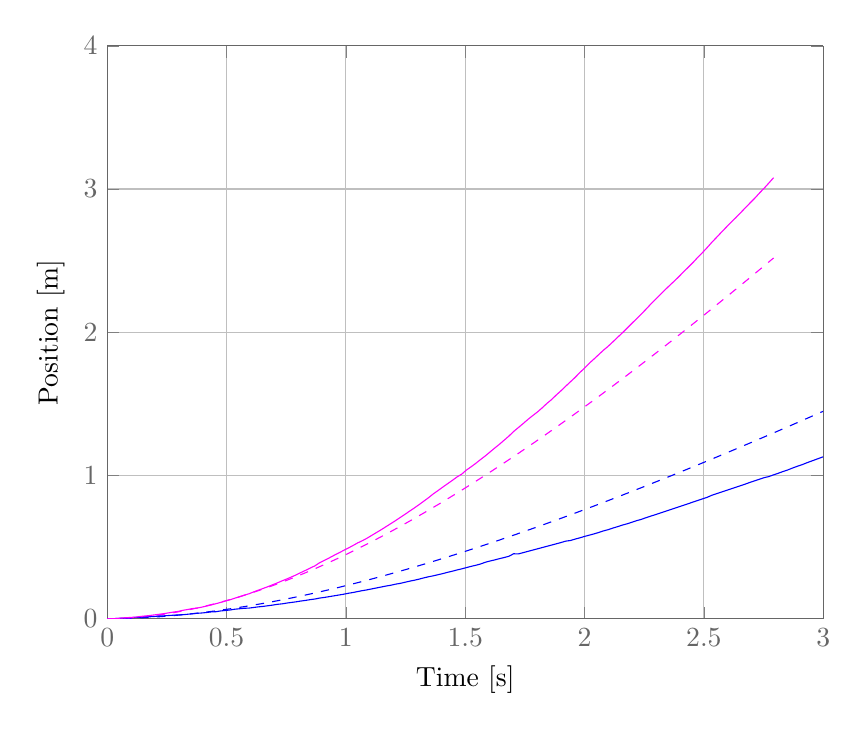
\begin{tikzpicture}

\begin{axis}[%
width=0.75\textwidth,
height=0.6\textwidth,
scale only axis,
separate axis lines,
every outer x axis line/.append style={white!40!black},
every x tick label/.append style={font=\color{white!40!black}},
xmin=0,
xmax=3,
xmajorgrids,
xlabel={Time [s]},
every outer y axis line/.append style={white!40!black},
every y tick label/.append style={font=\color{white!40!black}},
ymin=0,
ymax=4,
ymajorgrids,
ylabel={Position [m]},
axis background/.style={fill=white},
%legend style={at={(0.97,0.03)},anchor=south east,legend cell align=left,align=left,draw=black}
]
\addplot [color=blue,dashed]
  table[row sep=crcr]{%
0	0\\
0.0198000198000198	0.000117371982093649\\
0.0396000396000396	0.000467198587515959\\
0.0594000594000594	0.00104592099734742\\
0.0792000792000792	0.00184983314546589\\
0.099000099000099	0.00287510691776669\\
0.118800118800119	0.00411781840981444\\
0.138600138600139	0.00557397474629027\\
0.158400158400158	0.00723954098599551\\
0.178200178200178	0.00911046666309538\\
0.198000198000198	0.011182711547912\\
0.217800217800218	0.0134522702480346\\
0.237600237600238	0.0159151953119145\\
0.257400257400257	0.0185676185415437\\
0.277200277200277	0.0214057702673806\\
0.297000297000297	0.0244259963865006\\
0.316800316800317	0.0276247730131596\\
0.336600336600337	0.0309987186387668\\
0.356400356400356	0.0345446037449006\\
0.376200376200376	0.0382593578578044\\
0.396000396000396	0.0421400740751169\\
0.415800415800416	0.0461840111349201\\
0.435600435600436	0.0503885931330279\\
0.455400455400455	0.0547514070264512\\
0.475200475200475	0.0592701980888335\\
0.495000495000495	0.0639428635071779\\
0.514800514800515	0.0687674443282327\\
0.534600534600535	0.0737421159774428\\
0.554400554400554	0.0788651775834247\\
0.574200574200574	0.0841350403465974\\
0.594000594000594	0.0895502151920606\\
0.613800613800614	0.0951092999442825\\
0.633600633600634	0.100810966254923\\
0.653400653400653	0.106653946505489\\
0.673200673200673	0.112637020893866\\
0.693000693000693	0.118759004898454\\
0.712800712800713	0.125018737296104\\
0.732600732600733	0.131415068890667\\
0.752400752400752	0.137946852088214\\
0.772200772200772	0.14461293143322\\
0.792000792000792	0.1514121351977\\
0.811800811800812	0.158343268092783\\
0.831600831600832	0.165405105149925\\
0.851400851400851	0.17259638679724\\
0.871200871200871	0.179915815135537\\
0.891000891000891	0.187362051398984\\
0.910800910800911	0.194933714567001\\
0.930600930600931	0.202629381077348\\
0.95040095040095	0.210447585575473\\
0.97020097020097	0.218386822622299\\
0.99000099000099	0.226445549271692\\
1.00980100980101	0.234622188420048\\
1.02960102960103	0.242915132823749\\
1.04940104940105	0.25132274967559\\
1.06920106920107	0.259843385628732\\
1.08900108900109	0.26847537215609\\
1.10880110880111	0.277217031134356\\
1.12860112860113	0.286066680544765\\
1.14840114840115	0.295022640187317\\
1.16820116820117	0.304083237311067\\
1.18800118800119	0.313246812070327\\
1.20780120780121	0.322511722724789\\
1.22760122760123	0.331876350510696\\
1.24740124740125	0.341339104119852\\
1.26720126720127	0.350898423733452\\
1.28700128700129	0.360552784568118\\
1.30680130680131	0.370300699902026\\
1.32660132660133	0.380140723559401\\
1.34640134640135	0.390071451841778\\
1.36620136620137	0.400091524904155\\
1.38600138600139	0.410199627583343\\
1.40580140580141	0.420394489694282\\
1.42560142560143	0.430674885817913\\
1.44540144540145	0.441039634611024\\
1.46520146520147	0.451487597674545\\
1.48500148500149	0.462017678021794\\
1.5048015048015	0.472628818192252\\
1.52460152460152	0.483319998059567\\
1.54440154440154	0.49409023238456\\
1.56420156420156	0.504938568165243\\
1.58400158400158	0.515864081836034\\
1.6038016038016	0.52686587636783\\
1.62360162360162	0.537943078319116\\
1.64340164340164	0.549094834886185\\
1.66320166320166	0.560320310997745\\
1.68300168300168	0.571618686495795\\
1.7028017028017	0.582989153440829\\
1.72260172260172	0.594430913575186\\
1.74240174240174	0.605943175973792\\
1.76220176220176	0.617525154906857\\
1.78200178200178	0.62917606793415\\
1.8018018018018	0.640895134245664\\
1.82160182160182	0.652681573258549\\
1.84140184140184	0.664534603475566\\
1.86120186120186	0.676453441605695\\
1.88100188100188	0.688437301943348\\
1.9008019008019	0.700485395998615\\
1.92060192060192	0.712596932367409\\
1.94040194040194	0.724771116827157\\
1.96020196020196	0.737007152640892\\
1.98000198000198	0.749304241050275\\
1.999801999802	0.761661581936187\\
2.01960201960202	0.774078374624081\\
2.03940203940204	0.786553818810351\\
2.05920205920206	0.799087115585408\\
2.07900207900208	0.811677468529066\\
2.0988020988021	0.824324084854138\\
2.11860211860212	0.837026176574811\\
2.13840213840214	0.849782961677379\\
2.15820215820216	0.862593665272231\\
2.17800217800218	0.875457520707578\\
2.1978021978022	0.888373770627184\\
2.21760221760222	0.901341667956384\\
2.23740223740224	0.914360476802757\\
2.25720225720226	0.927429473260074\\
2.27700227700228	0.94054794610638\\
2.2968022968023	0.953715197389376\\
2.31660231660232	0.966930542894512\\
2.33640233640234	0.98019331249341\\
2.35620235620236	0.993502850372339\\
2.37600237600238	1.00685851514245\\
2.3958023958024	1.02025967983534\\
2.41560241560242	1.03370573178913\\
2.43540243540244	1.0471960724318\\
2.45520245520246	1.06073011696986\\
2.47500247500248	1.07430729399124\\
2.49480249480249	1.08792704499263\\
2.51460251460251	1.10158882384169\\
2.53440253440253	1.11529209618533\\
2.55420255420255	1.12903633881526\\
2.57400257400257	1.14282103900231\\
2.59380259380259	1.15664569381055\\
2.61360261360261	1.17050980940226\\
2.63340263340263	1.18441290034412\\
2.65320265320265	1.19835448892432\\
2.67300267300267	1.21233410448979\\
2.69280269280269	1.22635128281168\\
2.71260271260271	1.24040556548637\\
2.73240273240273	1.25449649937836\\
2.75220275220275	1.26862363611018\\
2.77200277200277	1.28278653160369\\
2.79180279180279	1.29698474567574\\
2.81160281160281	1.31121784169037\\
2.83140283140283	1.32548538626855\\
2.85120285120285	1.33978694905556\\
2.87100287100287	1.35412210254516\\
2.89080289080289	1.36849042195882\\
2.91060291060291	1.38289148517758\\
2.93040293040293	1.39732487272328\\
2.95020295020295	1.41179016778545\\
2.97000297000297	1.42628695628955\\
2.98980298980299	1.44081482700188\\
3.00960300960301	1.45537337166625\\
3.02940302940303	1.46996218516703\\
3.04920304920305	1.48458086571351\\
3.06900306900307	1.49922901504009\\
3.08880308880309	1.51390623861714\\
3.10860310860311	1.52861214586738\\
3.12840312840313	1.54334635038295\\
3.14820314820315	1.55810847013859\\
3.16800316800317	1.57289812769669\\
3.18780318780319	1.5877149504004\\
3.20760320760321	1.60255857055129\\
3.22740322740323	1.61742862556883\\
3.24720324720325	1.63232475812905\\
3.26700326700327	1.64724661628051\\
3.28680328680329	1.66219385353608\\
3.30660330660331	1.67716612893961\\
3.32640332640333	1.69216310710698\\
3.34620334620335	1.70718445824142\\
3.36600336600337	1.72222985812363\\
3.38580338580339	1.73729898807739\\
3.40560340560341	1.75239153491187\\
3.42540342540343	1.76750719084206\\
3.44520344520345	1.78264565338915\\
3.46500346500346	1.7978066252628\\
3.48480348480348	1.81298981422748\\
3.5046035046035	1.82819493295522\\
3.52440352440352	1.84342169886712\\
3.54420354420354	1.8586698339662\\
3.56400356400356	1.8739390646639\\
3.58380358380358	1.88922912160276\\
3.6036036036036	1.90453973947765\\
3.62340362340362	1.91987065685775\\
3.64320364320364	1.93522161601138\\
3.66300366300366	1.95059236273578\\
3.68280368280368	1.96598264619338\\
3.7026037026037	1.98139221875631\\
3.72240372240372	1.99682083586045\\
3.74220374220374	2.01226825587013\\
3.76200376200376	2.02773423995431\\
3.78180378180378	2.04321855197505\\
3.8016038016038	2.0587209583886\\
3.82140382140382	2.0742412281593\\
3.84120384120384	2.08977913268635\\
3.86100386100386	2.10533444574324\\
3.88080388080388	2.12090694342945\\
3.9006039006039	2.13649640413378\\
3.92040392040392	2.15210260850874\\
3.94020394020394	2.16772533945509\\
3.96000396000396	2.18336438211558\\
3.97980397980398	2.1990195238769\\
3.999603999604	2.21469055437873\\
4.01940401940402	2.23037726552871\\
4.03920403920404	2.24607945152233\\
4.05900405900406	2.26179690886628\\
4.07880407880408	2.27752943640452\\
4.0986040986041	2.29327683534552\\
4.11840411840412	2.30903890929006\\
4.13820413820414	2.32481546425816\\
4.15800415800416	2.34060630871458\\
4.17780417780418	2.35641125359182\\
4.1976041976042	2.37223011231005\\
4.21740421740422	2.38806270079317\\
4.23720423720424	2.40390883748065\\
4.25700425700426	2.41976834333455\\
4.27680427680428	2.43564104184156\\
4.2966042966043	2.45152675900974\\
4.31640431640432	2.46742532335995\\
4.33620433620434	2.48333656591189\\
4.35600435600436	2.49926032016485\\
4.37580437580438	2.51519642207341\\
4.3956043956044	2.53114471001826\\
4.41540441540442	2.54710502477257\\
4.43520443520443	2.56307720946409\\
4.45500445500446	2.5790611095337\\
4.47480447480447	2.59505657269068\\
4.49460449460449	2.61106344886515\\
4.51440451440451	2.6270815901585\\
4.53420453420453	2.64311085079199\\
4.55400455400455	2.65915108705431\\
4.57380457380457	2.67520215724847\\
4.59360459360459	2.69126392163861\\
4.61340461340461	2.70733624239726\\
4.63320463320463	2.7234189835533\\
4.65300465300465	2.73951201094136\\
4.67280467280467	2.7556151921527\\
4.69260469260469	2.77172839648818\\
4.71240471240471	2.78785149491345\\
4.73220473220473	2.80398436001666\\
4.75200475200475	2.82012686596883\\
4.77180477180477	2.8362788884871\\
4.79160479160479	2.85244030480089\\
4.81140481140481	2.86861099362098\\
4.83120483120483	2.88479083511161\\
4.85100485100485	2.90097971086542\\
4.87080487080487	2.91717750388126\\
4.89060489060489	2.93338409854467\\
4.91040491040491	2.94959938061088\\
4.93020493020493	2.9658232371902\\
4.95000495000495	2.98205555673549\\
4.96980496980497	2.99829622903159\\
4.98960498960499	3.01454514518643\\
5.00940500940501	3.03080219762353\\
5.02920502920503	3.04706728007565\\
5.04900504900505	3.06334028757945\\
5.06880506880507	3.07962111647071\\
5.08860508860509	3.09590966438\\
5.10840510840511	3.11220583022862\\
5.12820512820513	3.12850951422437\\
5.14800514800515	3.14482061785725\\
5.16780516780517	3.1611390438946\\
5.18760518760519	3.17746469637581\\
5.20740520740521	3.19379748060623\\
5.22720522720523	3.21013730315026\\
5.24700524700525	3.22648407182363\\
5.26680526680527	3.24283769568455\\
5.28660528660529	3.25919808502393\\
5.30640530640531	3.27556515135455\\
5.32620532620533	3.29193880739913\\
5.34600534600535	3.30831896707737\\
5.36580536580537	3.3247055454921\\
5.38560538560538	3.34109845891434\\
5.40540540540541	3.35749762476761\\
5.42520542520542	3.37390296161138\\
5.44500544500545	3.3903143891239\\
5.46480546480546	3.40673182808435\\
5.48460548460548	3.42315520035462\\
5.5044055044055	3.4395844288606\\
5.52420552420552	3.45601943757333\\
5.54400554400554	3.47246015148991\\
5.56380556380556	3.4889064966145\\
5.58360558360558	3.50535839993925\\
5.6034056034056	3.52181578942558\\
5.62320562320562	3.53827859398563\\
5.64300564300564	3.55474674346415\\
5.66280566280566	3.5712201686208\\
5.68260568260568	3.587698801113\\
5.7024057024057	3.60418257347938\\
5.72220572220572	3.62067141912383\\
5.74200574200574	3.63716527230027\\
5.76180576180576	3.6536640680981\\
5.78160578160578	3.67016774242837\\
5.8014058014058	3.6866762320107\\
5.82120582120582	3.70318947436088\\
5.84100584100584	3.71970740777926\\
5.86080586080586	3.73622997133976\\
5.88060588060588	3.75275710487959\\
5.9004059004059	3.76928874898955\\
5.92020592020592	3.785824845005\\
5.94000594000594	3.80236533499726\\
5.95980595980596	3.81891016176561\\
5.97960597960598	3.83545926882962\\
5.999405999406	3.85201260042196\\
6.01920601920602	3.86857010148144\\
6.03900603900604	3.88513171764642\\
6.05880605880606	3.9016973952483\\
6.07860607860608	3.91826708130533\\
6.0984060984061	3.93484072351637\\
6.11820611820612	3.95141827025483\\
6.13800613800614	3.96799967056255\\
6.15780615780616	3.9845848741437\\
6.17760617760618	4.00117383135858\\
};
%\addlegendentry{1A model};

\addplot [color=mycolor3,dashed]
  table[row sep=crcr]{%
0	0\\
0.0198000198000198	0.000227892410235163\\
0.0396000396000396	0.00090712459880352\\
0.0594000594000594	0.00203078667284401\\
0.0792000792000792	0.00359168284060122\\
0.099000099000099	0.00558238033886875\\
0.118800118800119	0.0079952604155103\\
0.138600138600139	0.0108225704027772\\
0.158400158400158	0.014056475956744\\
0.178200178200178	0.0176891125904591\\
0.198000198000198	0.021712635691752\\
0.217800217800218	0.0261192682893718\\
0.237600237600238	0.0309013459115112\\
0.257400257400257	0.0360513579670428\\
0.277200277200277	0.0415619851702028\\
0.297000297000297	0.0474261326222946\\
0.316800316800317	0.0536369582575948\\
0.336600336600337	0.0601878964534626\\
0.356400356400356	0.0670726766952162\\
0.376200376200376	0.0742853372733187\\
0.396000396000396	0.0818202340725941\\
0.415800415800416	0.0896720445895411\\
0.435600435600436	0.0978357673834158\\
0.455400455400455	0.106306717228894\\
0.475200475200475	0.115080516292232\\
0.495000495000495	0.124153081698509\\
0.514800514800515	0.133520609894525\\
0.534600534600535	0.143179558240157\\
0.554400554400554	0.153126624280491\\
0.574200574200574	0.16335872316206\\
0.594000594000594	0.173872963659361\\
0.613800613800614	0.184666623272901\\
0.633600633600634	0.195737122847933\\
0.653400653400653	0.207082001144318\\
0.673200673200673	0.218698889763406\\
0.693000693000693	0.230585488808087\\
0.712800712800713	0.242739543618113\\
0.732600732600733	0.255158822885164\\
0.752400752400752	0.267841098411829\\
0.772200772200772	0.280784126736427\\
0.792000792000792	0.293985632802253\\
0.811800811800812	0.307443295806191\\
0.831600831600832	0.321154737318324\\
0.851400851400851	0.335117511722005\\
0.871200871200871	0.349329098983326\\
0.891000891000891	0.363786899720672\\
0.910800910800911	0.378488232509544\\
0.930600930600931	0.393430333325475\\
0.95040095040095	0.40861035699899\\
0.97020097020097	0.42402538053149\\
0.99000099000099	0.439672408099714\\
1.00980100980101	0.455548377559404\\
1.02960102960103	0.471650168245682\\
1.04940104940105	0.487974609858768\\
1.06920106920107	0.504518492218601\\
1.08900108900109	0.521278575670779\\
1.10880110880111	0.538251601928625\\
1.12860112860113	0.555434305141945\\
1.14840114840115	0.572823422991905\\
1.16820116820117	0.590415707622949\\
1.18800118800119	0.608207936236687\\
1.20780120780121	0.6261969211886\\
1.22760122760123	0.644379519446017\\
1.24740124740125	0.662752641284681\\
1.26720126720127	0.681313258120932\\
1.28700128700129	0.700058409396782\\
1.30680130680131	0.718985208455524\\
1.32660132660133	0.738090847365678\\
1.34640134640135	0.757372600670785\\
1.36620136620137	0.776827828061388\\
1.38600138600139	0.796453975983356\\
1.40580140580141	0.816248578213241\\
1.42560142560143	0.836209255446392\\
1.44540144540145	0.856333713956937\\
1.46520146520147	0.876619743400438\\
1.48500148500149	0.897065213839795\\
1.5048015048015	0.91766807208291\\
1.52460152460152	0.938426337426644\\
1.54440154440154	0.959338096905681\\
1.56420156420156	0.980401500147244\\
1.58400158400158	1.00161475393304\\
1.6038016038016	1.02297611656865\\
1.62360162360162	1.04448389215794\\
1.64340164340164	1.06613642487565\\
1.66320166320166	1.08793209332623\\
1.68300168300168	1.10986930507015\\
1.7028017028017	1.13194649139163\\
1.72260172260172	1.1541621023734\\
1.74240174240174	1.17651460233531\\
1.76220176220176	1.19900246568453\\
1.78200178200178	1.22162417321531\\
1.8018018018018	1.24437820888717\\
1.82160182160182	1.26726305710072\\
1.84140184140184	1.29027720048113\\
1.86120186120186	1.31341911817074\\
1.88100188100188	1.33668728462371\\
1.9008019008019	1.36008016888806\\
1.92060192060192	1.38359623435361\\
1.94040194040194	1.4072339389377\\
1.96020196020196	1.43099173567569\\
1.98000198000198	1.45486807367817\\
1.999801999802	1.47886139941362\\
2.01960201960202	1.50297015827207\\
2.03940203940204	1.5271927963638\\
2.05920205920206	1.55152776250574\\
2.07900207900208	1.57597351034828\\
2.0988020988021	1.60052850059579\\
2.11860211860212	1.62519120327506\\
2.13840213840214	1.6499601000085\\
2.15820215820216	1.67483368625082\\
2.17800217800218	1.69981047345153\\
2.1978021978022	1.72488899110858\\
2.21760221760222	1.7500677886829\\
2.23740223740224	1.77534543734716\\
2.25720225720226	1.8007205315467\\
2.27700227700228	1.82619169035497\\
2.2968022968023	1.85175755861014\\
2.31660231660232	1.87741680782392\\
2.33640233640234	1.90316813685809\\
2.35620235620236	1.92901027236812\\
2.37600237600238	1.9549419690172\\
2.3958023958024	1.98096200946761\\
2.41560241560242	2.00706920415952\\
2.43540243540244	2.03326239089041\\
2.45520245520246	2.05954043421038\\
2.47500247500248	2.08590222465133\\
2.49480249480249	2.11234667780909\\
2.51460251460251	2.13887273329931\\
2.53440253440253	2.16547935360848\\
2.55420255420255	2.19216552286217\\
2.57400257400257	2.21893024553244\\
2.59380259380259	2.24577254510615\\
2.61360261360261	2.27269146273552\\
2.63340263340263	2.2996860558909\\
2.65320265320265	2.32675539703496\\
2.67300267300267	2.35389857233581\\
2.69280269280269	2.38111468043496\\
2.71260271260271	2.40840283128434\\
2.73240273240273	2.43576214506458\\
2.75220275220275	2.46319175119466\\
2.77200277200277	2.49069078744123\\
2.79180279180279	2.51825839913354\\
};
%\addlegendentry{2A model};

\addplot [color=blue,solid]
  table[row sep=crcr]{%
0	-0.00109999999999999\\
0.0198000198000198	5.55111512312578e-17\\
0.0396000396000396	0.00110000000000005\\
0.0594000594000594	0.00330000000000003\\
0.0792000792000792	0.00440000000000002\\
0.099000099000099	0.00660000000000005\\
0.118800118800119	0.00880000000000003\\
0.138600138600139	0.00990000000000002\\
0.158400158400158	0.0121000000000001\\
0.178200178200178	0.0132\\
0.198000198000198	0.0154\\
0.217800217800218	0.0187000000000001\\
0.237600237600238	0.0198\\
0.257400257400257	0.022\\
0.277200277200277	0.0242000000000001\\
0.297000297000297	0.0264\\
0.316800316800317	0.0275\\
0.336600336600337	0.0308000000000001\\
0.356400356400356	0.0341\\
0.376200376200376	0.0374\\
0.396000396000396	0.0396\\
0.415800415800416	0.0429\\
0.435600435600436	0.0473\\
0.455400455400455	0.0484000000000001\\
0.475200475200475	0.0539000000000001\\
0.495000495000495	0.0572\\
0.514800514800515	0.0605000000000001\\
0.534600534600535	0.0660000000000001\\
0.554400554400554	0.0693\\
0.574200574200574	0.0726000000000001\\
0.594000594000594	0.0737\\
0.613800613800614	0.0781000000000001\\
0.633600633600634	0.0825\\
0.653400653400653	0.0858\\
0.673200673200673	0.0902000000000001\\
0.693000693000693	0.0946\\
0.712800712800713	0.1001\\
0.732600732600733	0.1034\\
0.752400752400752	0.1089\\
0.772200772200772	0.1133\\
0.792000792000792	0.1177\\
0.811800811800812	0.1232\\
0.831600831600832	0.1276\\
0.851400851400851	0.1331\\
0.871200871200871	0.1375\\
0.891000891000891	0.1441\\
0.910800910800911	0.1485\\
0.930600930600931	0.154\\
0.95040095040095	0.1595\\
0.97020097020097	0.165\\
0.99000099000099	0.1705\\
1.00980100980101	0.1771\\
1.02960102960103	0.1826\\
1.04940104940105	0.1892\\
1.06920106920107	0.1958\\
1.08900108900109	0.2013\\
1.10880110880111	0.2079\\
1.12860112860113	0.2145\\
1.14840114840115	0.2211\\
1.16820116820117	0.2277\\
1.18800118800119	0.2332\\
1.20780120780121	0.2409\\
1.22760122760123	0.2464\\
1.24740124740125	0.2541\\
1.26720126720127	0.2618\\
1.28700128700129	0.2684\\
1.30680130680131	0.2761\\
1.32660132660133	0.2849\\
1.34640134640135	0.2926\\
1.36620136620137	0.2992\\
1.38600138600139	0.3069\\
1.40580140580141	0.3146\\
1.42560142560143	0.3234\\
1.44540144540145	0.3311\\
1.46520146520147	0.3399\\
1.48500148500149	0.3476\\
1.5048015048015	0.3564\\
1.52460152460152	0.3652\\
1.54440154440154	0.3729\\
1.56420156420156	0.3817\\
1.58400158400158	0.3938\\
1.6038016038016	0.4026\\
1.62360162360162	0.4103\\
1.64340164340164	0.4191\\
1.66320166320166	0.4268\\
1.68300168300168	0.4356\\
1.7028017028017	0.4532\\
1.72260172260172	0.4521\\
1.74240174240174	0.4609\\
1.76220176220176	0.4697\\
1.78200178200178	0.4785\\
1.8018018018018	0.4873\\
1.82160182160182	0.4961\\
1.84140184140184	0.5049\\
1.86120186120186	0.5137\\
1.88100188100188	0.5225\\
1.9008019008019	0.5313\\
1.92060192060192	0.5412\\
1.94040194040194	0.5456\\
1.96020196020196	0.5555\\
1.98000198000198	0.5643\\
1.999801999802	0.5742\\
2.01960201960202	0.583\\
2.03940203940204	0.5918\\
2.05920205920206	0.6017\\
2.07900207900208	0.6127\\
2.0988020988021	0.6215\\
2.11860211860212	0.6325\\
2.13840213840214	0.6424\\
2.15820215820216	0.6534\\
2.17800217800218	0.6622\\
2.1978021978022	0.6732\\
2.21760221760222	0.6842\\
2.23740223740224	0.693\\
2.25720225720226	0.7051\\
2.27700227700228	0.7161\\
2.2968022968023	0.726\\
2.31660231660232	0.737\\
2.33640233640234	0.748\\
2.35620235620236	0.759\\
2.37600237600238	0.77\\
2.3958023958024	0.781\\
2.41560241560242	0.792\\
2.43540243540244	0.803\\
2.45520245520246	0.8151\\
2.47500247500248	0.8261\\
2.49480249480249	0.8371\\
2.51460251460251	0.8481\\
2.53440253440253	0.8624\\
2.55420255420255	0.8734\\
2.57400257400257	0.8844\\
2.59380259380259	0.8954\\
2.61360261360261	0.9064\\
2.63340263340263	0.9174\\
2.65320265320265	0.9284\\
2.67300267300267	0.9394\\
2.69280269280269	0.9515\\
2.71260271260271	0.9625\\
2.73240273240273	0.9735\\
2.75220275220275	0.9845\\
2.77200277200277	0.9922\\
2.79180279180279	1.0043\\
2.81160281160281	1.0153\\
2.83140283140283	1.0274\\
2.85120285120285	1.0384\\
2.87100287100287	1.0516\\
2.89080289080289	1.0637\\
2.91060291060291	1.0747\\
2.93040293040293	1.0879\\
2.95020295020295	1.1\\
2.97000297000297	1.1121\\
2.98980298980299	1.1242\\
3.00960300960301	1.1363\\
3.02940302940303	1.1484\\
3.04920304920305	1.1627\\
3.06900306900307	1.1748\\
3.08880308880309	1.188\\
3.10860310860311	1.2012\\
3.12840312840313	1.2133\\
3.14820314820315	1.2265\\
3.16800316800317	1.2408\\
3.18780318780319	1.254\\
3.20760320760321	1.2672\\
3.22740322740323	1.2804\\
3.24720324720325	1.2936\\
3.26700326700327	1.3101\\
3.28680328680329	1.3222\\
3.30660330660331	1.3354\\
3.32640332640333	1.3475\\
3.34620334620335	1.3596\\
3.36600336600337	1.3728\\
3.38580338580339	1.386\\
3.40560340560341	1.3981\\
3.42540342540343	1.4113\\
3.44520344520345	1.4234\\
3.46500346500346	1.4322\\
3.48480348480348	1.4454\\
3.5046035046035	1.4608\\
3.52440352440352	1.4729\\
3.54420354420354	1.4861\\
3.56400356400356	1.5004\\
3.58380358380358	1.5136\\
3.6036036036036	1.5257\\
3.62340362340362	1.5389\\
3.64320364320364	1.5532\\
3.66300366300366	1.5664\\
3.68280368280368	1.5796\\
3.7026037026037	1.5939\\
3.72240372240372	1.6071\\
3.74220374220374	1.6214\\
3.76200376200376	1.6346\\
3.78180378180378	1.6478\\
3.8016038016038	1.6621\\
3.82140382140382	1.6764\\
3.84120384120384	1.6896\\
3.86100386100386	1.705\\
3.88080388080388	1.7182\\
3.9006039006039	1.7325\\
3.92040392040392	1.7468\\
3.94020394020394	1.7622\\
3.96000396000396	1.7765\\
3.97980397980398	1.7886\\
3.999603999604	1.8018\\
4.01940401940402	1.815\\
4.03920403920404	1.8293\\
4.05900405900406	1.8414\\
4.07880407880408	1.8546\\
4.0986040986041	1.8678\\
4.11840411840412	1.881\\
4.13820413820414	1.8909\\
4.15800415800416	1.903\\
4.17780417780418	1.9162\\
4.1976041976042	1.9305\\
4.21740421740422	1.9426\\
4.23720423720424	1.9558\\
4.25700425700426	1.969\\
4.27680427680428	1.9811\\
4.2966042966043	1.9932\\
4.31640431640432	2.0075\\
4.33620433620434	2.0218\\
4.35600435600436	2.035\\
4.37580437580438	2.0471\\
4.3956043956044	2.0603\\
4.41540441540442	2.0735\\
4.43520443520443	2.0856\\
4.45500445500446	2.0988\\
4.47480447480447	2.1131\\
4.4946044946045	2.1252\\
4.51440451440451	2.1384\\
4.53420453420453	2.1516\\
4.55400455400455	2.1648\\
4.57380457380457	2.1791\\
4.59360459360459	2.1923\\
4.61340461340461	2.2044\\
4.63320463320463	2.2187\\
4.65300465300465	2.2308\\
4.67280467280467	2.2429\\
4.69260469260469	2.255\\
4.71240471240471	2.2671\\
4.73220473220473	2.2792\\
4.75200475200475	2.2924\\
4.77180477180477	2.3034\\
4.79160479160479	2.3155\\
4.81140481140481	2.3276\\
4.83120483120483	2.3386\\
4.85100485100485	2.3496\\
4.87080487080487	2.3606\\
4.89060489060489	2.3738\\
4.91040491040491	2.3848\\
4.93020493020493	2.3969\\
4.95000495000495	2.409\\
4.96980496980497	2.42\\
4.98960498960499	2.431\\
5.00940500940501	2.442\\
5.02920502920503	2.4541\\
5.04900504900505	2.4662\\
5.06880506880507	2.4772\\
5.08860508860509	2.4904\\
5.10840510840511	2.5025\\
5.12820512820513	2.5146\\
5.14800514800515	2.5256\\
5.16780516780517	2.5366\\
5.18760518760519	2.5476\\
5.20740520740521	2.5586\\
5.22720522720523	2.5707\\
5.24700524700525	2.5817\\
5.26680526680527	2.5938\\
5.28660528660529	2.6059\\
5.30640530640531	2.6191\\
5.32620532620533	2.6301\\
5.34600534600535	2.6411\\
5.36580536580537	2.6521\\
5.38560538560539	2.662\\
5.40540540540541	2.673\\
5.42520542520543	2.684\\
5.44500544500545	2.695\\
5.46480546480546	2.706\\
5.48460548460548	2.7159\\
5.5044055044055	2.7258\\
5.52420552420552	2.7357\\
5.54400554400554	2.7456\\
5.56380556380556	2.7566\\
5.58360558360558	2.7665\\
5.6034056034056	2.7764\\
5.62320562320562	2.7841\\
5.64300564300564	2.794\\
5.66280566280566	2.8028\\
5.68260568260568	2.8127\\
5.7024057024057	2.8226\\
5.72220572220572	2.8325\\
5.74200574200574	2.8424\\
5.76180576180576	2.8523\\
5.78160578160578	2.86\\
5.8014058014058	2.8688\\
5.82120582120582	2.8787\\
5.84100584100584	2.8875\\
5.86080586080586	2.8985\\
5.88060588060588	2.9062\\
5.9004059004059	2.915\\
5.92020592020592	2.9227\\
5.94000594000594	2.9326\\
5.95980595980596	2.9403\\
5.97960597960598	2.9491\\
5.999405999406	2.9568\\
6.01920601920602	2.9667\\
6.03900603900604	2.9755\\
6.05880605880606	2.9843\\
6.07860607860608	2.9931\\
6.0984060984061	3.0019\\
6.11820611820612	3.0107\\
6.13800613800614	3.0184\\
6.15780615780616	3.0261\\
6.17760617760618	3.0349\\
6.1974061974062	3.0437\\
6.21720621720622	3.0514\\
6.23700623700624	3.0602\\
6.25680625680626	3.0679\\
6.27660627660628	3.0767\\
6.2964062964063	3.0844\\
6.31620631620632	3.091\\
6.33600633600634	3.0987\\
6.35580635580636	3.1064\\
6.37560637560638	3.1141\\
6.3954063954064	3.1218\\
6.41520641520642	3.1284\\
6.43500643500643	3.1361\\
6.45480645480646	3.1427\\
6.47460647460647	3.1504\\
6.49440649440649	3.1581\\
6.51420651420651	3.1658\\
6.53400653400653	3.1724\\
6.55380655380655	3.1779\\
6.57360657360657	3.1845\\
6.59340659340659	3.1911\\
6.61320661320661	3.1977\\
6.63300663300663	3.2032\\
6.65280665280665	3.2098\\
6.67260667260667	3.2164\\
6.69240669240669	3.223\\
6.71220671220671	3.2296\\
6.73200673200673	3.2351\\
6.75180675180675	3.2417\\
6.77160677160677	3.2472\\
6.79140679140679	3.2538\\
6.81120681120681	3.2593\\
6.83100683100683	3.2659\\
6.85080685080685	3.2714\\
6.87060687060687	3.2769\\
6.89040689040689	3.2824\\
6.91020691020691	3.2879\\
6.93000693000693	3.2934\\
6.94980694980695	3.2989\\
6.96960696960697	3.3044\\
6.98940698940699	3.3099\\
7.00920700920701	3.3165\\
7.02900702900703	3.3209\\
7.04880704880705	3.3275\\
7.06860706860707	3.3319\\
7.08840708840709	3.3363\\
7.10820710820711	3.3429\\
7.12800712800713	3.3473\\
7.14780714780715	3.3506\\
7.16760716760717	3.355\\
7.18740718740719	3.3616\\
7.20720720720721	3.366\\
7.22700722700723	3.3682\\
7.24680724680725	3.3737\\
7.26660726660727	3.3803\\
7.28640728640729	3.3825\\
7.30620730620731	3.3891\\
7.32600732600733	3.3924\\
7.34580734580735	3.3979\\
7.36560736560737	3.4012\\
7.38540738540739	3.4067\\
7.40520740520741	3.4111\\
7.42500742500742	3.4155\\
7.44480744480745	3.4188\\
7.46460746460746	3.421\\
7.48440748440748	3.4265\\
7.5042075042075	3.4287\\
7.52400752400752	3.4331\\
7.54380754380754	3.4364\\
7.56360756360756	3.4397\\
7.58340758340758	3.443\\
7.6032076032076	3.4463\\
7.62300762300762	3.4496\\
7.64280764280764	3.4529\\
7.66260766260766	3.4562\\
7.68240768240768	3.4595\\
7.7022077022077	3.4628\\
7.72200772200772	3.4661\\
7.74180774180774	3.4694\\
7.76160776160776	3.4727\\
7.78140778140778	3.476\\
7.8012078012078	3.4782\\
7.82100782100782	3.4815\\
7.84080784080784	3.4837\\
7.86060786060786	3.487\\
7.88040788040788	3.4903\\
7.9002079002079	3.4925\\
7.92000792000792	3.4958\\
7.93980793980794	3.498\\
7.95960795960796	3.5013\\
7.97940797940798	3.5035\\
7.999207999208	3.5057\\
8.01900801900802	3.509\\
8.03880803880804	3.5112\\
8.05860805860806	3.5145\\
8.07840807840808	3.5167\\
8.0982080982081	3.5189\\
8.11800811800812	3.5211\\
8.13780813780814	3.5244\\
8.15760815760816	3.5266\\
8.17740817740818	3.5288\\
8.1972081972082	3.531\\
8.21700821700822	3.5321\\
8.23680823680824	3.5343\\
8.25660825660826	3.5365\\
8.27640827640828	3.5376\\
8.2962082962083	3.5398\\
8.31600831600832	3.5409\\
8.33580833580834	3.5431\\
8.35560835560836	3.5442\\
8.37540837540837	3.5453\\
8.3952083952084	3.5464\\
8.41500841500842	3.5475\\
8.43480843480843	3.5486\\
8.45460845460845	3.5497\\
8.47440847440847	3.5497\\
8.4942084942085	3.5508\\
8.51400851400851	3.5508\\
8.53380853380853	3.5508\\
8.55360855360855	3.5519\\
8.57340857340857	3.5519\\
8.59320859320859	3.5519\\
8.61300861300861	3.5519\\
8.63280863280863	3.5519\\
8.65260865260865	3.5519\\
8.67240867240867	3.5519\\
8.69220869220869	3.5519\\
8.71200871200871	3.5519\\
8.73180873180873	3.5519\\
8.75160875160875	3.5519\\
8.77140877140877	3.5519\\
8.79120879120879	3.553\\
8.81100881100881	3.553\\
8.83080883080883	3.553\\
8.85060885060885	3.5519\\
8.87040887040887	3.553\\
8.89020889020889	3.553\\
8.91000891000891	3.5519\\
8.92980892980893	3.553\\
8.94960894960895	3.553\\
8.96940896940897	3.553\\
8.98920898920899	3.5519\\
9.00900900900901	3.553\\
};
%\addlegendentry{1A samples};

\addplot [color=mycolor3,solid]
  table[row sep=crcr]{%
0	-0.00109999999999996\\
0.0198000198000198	2.77555756156289e-17\\
0.0396000396000396	0.00110000000000002\\
0.0594000594000594	0.00440000000000004\\
0.0792000792000792	0.00660000000000002\\
0.099000099000099	0.0088\\
0.118800118800119	0.011\\
0.138600138600139	0.0154000000000001\\
0.158400158400158	0.0187\\
0.178200178200178	0.022\\
0.198000198000198	0.0264\\
0.217800217800218	0.0308\\
0.237600237600238	0.0352\\
0.257400257400257	0.0407\\
0.277200277200277	0.0462\\
0.297000297000297	0.0506\\
0.316800316800317	0.0583\\
0.336600336600337	0.0638000000000001\\
0.356400356400356	0.0704\\
0.376200376200376	0.0737\\
0.396000396000396	0.0803\\
0.415800415800416	0.0880000000000001\\
0.435600435600436	0.0957\\
0.455400455400455	0.1045\\
0.475200475200475	0.1133\\
0.495000495000495	0.1232\\
0.514800514800515	0.132\\
0.534600534600535	0.143\\
0.554400554400554	0.1529\\
0.574200574200574	0.1639\\
0.594000594000594	0.1738\\
0.613800613800614	0.187\\
0.633600633600634	0.1991\\
0.653400653400653	0.2112\\
0.673200673200673	0.2233\\
0.693000693000693	0.2365\\
0.712800712800713	0.2497\\
0.732600732600733	0.264\\
0.752400752400752	0.2772\\
0.772200772200772	0.2915\\
0.792000792000792	0.3058\\
0.811800811800812	0.3223\\
0.831600831600832	0.3377\\
0.851400851400851	0.3542\\
0.871200871200871	0.3696\\
0.891000891000891	0.3916\\
0.910800910800911	0.4081\\
0.930600930600931	0.4246\\
0.95040095040095	0.4422\\
0.97020097020097	0.4587\\
0.99000099000099	0.4763\\
1.00980100980101	0.4928\\
1.02960102960103	0.5104\\
1.04940104940105	0.5291\\
1.06920106920107	0.5445\\
1.08900108900109	0.5621\\
1.10880110880111	0.5819\\
1.12860112860113	0.6017\\
1.14840114840115	0.6215\\
1.16820116820117	0.6424\\
1.18800118800119	0.6633\\
1.20780120780121	0.6842\\
1.22760122760123	0.7062\\
1.24740124740125	0.7282\\
1.26720126720127	0.7513\\
1.28700128700129	0.7733\\
1.30680130680131	0.7964\\
1.32660132660133	0.8206\\
1.34640134640135	0.8448\\
1.36620136620137	0.8712\\
1.38600138600139	0.8943\\
1.40580140580141	0.9185\\
1.42560142560143	0.9416\\
1.44540144540145	0.9647\\
1.46520146520147	0.9889\\
1.48500148500149	1.0087\\
1.5048015048015	1.0373\\
1.52460152460152	1.0604\\
1.54440154440154	1.0846\\
1.56420156420156	1.111\\
1.58400158400158	1.1363\\
1.6038016038016	1.1638\\
1.62360162360162	1.1913\\
1.64340164340164	1.2177\\
1.66320166320166	1.2463\\
1.68300168300168	1.2749\\
1.7028017028017	1.3068\\
1.72260172260172	1.3343\\
1.74240174240174	1.3618\\
1.76220176220176	1.3904\\
1.78200178200178	1.4168\\
1.8018018018018	1.4421\\
1.82160182160182	1.4707\\
1.84140184140184	1.5015\\
1.86120186120186	1.529\\
1.88100188100188	1.5609\\
1.9008019008019	1.5906\\
1.92060192060192	1.6225\\
1.94040194040194	1.6533\\
1.96020196020196	1.6841\\
1.98000198000198	1.7182\\
1.999801999802	1.749\\
2.01960201960202	1.7831\\
2.03940203940204	1.8128\\
2.05920205920206	1.8436\\
2.07900207900208	1.8744\\
2.0988020988021	1.9019\\
2.11860211860212	1.9327\\
2.13840213840214	1.9646\\
2.15820215820216	1.9954\\
2.17800217800218	2.0284\\
2.1978021978022	2.0614\\
2.21760221760222	2.0933\\
2.23740223740224	2.1263\\
2.25720225720226	2.1604\\
2.27700227700228	2.1956\\
2.2968022968023	2.2286\\
2.31660231660232	2.2616\\
2.33640233640234	2.2946\\
2.35620235620236	2.3265\\
2.37600237600238	2.3573\\
2.3958023958024	2.3892\\
2.41560241560242	2.4233\\
2.43540243540244	2.4552\\
2.45520245520246	2.4882\\
2.47500247500248	2.5245\\
2.49480249480249	2.5575\\
2.51460251460251	2.5927\\
2.53440253440253	2.6301\\
2.55420255420255	2.6642\\
2.57400257400257	2.6994\\
2.59380259380259	2.7335\\
2.61360261360261	2.7676\\
2.63340263340263	2.7995\\
2.65320265320265	2.8336\\
2.67300267300267	2.8677\\
2.69280269280269	2.9018\\
2.71260271260271	2.9348\\
2.73240273240273	2.9711\\
2.75220275220275	3.0052\\
2.77200277200277	3.0415\\
2.79180279180279	3.0789\\
};
%\addlegendentry{2A samples};

\end{axis}

\begin{axis}[%
width=0.85\textwidth,
height=0.6\textwidth,
at={(1.85in,0.746in)},
scale only axis,
every outer x axis line/.append style={black},
every x tick label/.append style={font=\color{black}},
xmin=0,
xmax=1,
xtick={\empty},
every outer y axis line/.append style={black},
every y tick label/.append style={font=\color{black}},
ymin=0,
ymax=1,
ytick={\empty},
hide axis,
axis x line*=bottom,
axis y line*=left
]
\end{axis}
\end{tikzpicture}%
              \end{figure}}  
        \item<2-> Dæmper 
        \item<2-> Inerti / masse       
    \end{itemize}           
  \end{minipage}
  \begin{minipage}[t]{0.48\linewidth} 
    \begin{itemize}            
	\item<3->[] {
              \begin{figure}[H]
              \centering
              \input{Billeder/Daniel/senstools_X-axis_2A.tex}
              \end{figure}}	     	
    \end{itemize}           
  \end{minipage}
\end{frame} 
%%%%%%%%%%%%%%%%

\begin{frame}{Model opstilling}{Trolley- og pendulmodel}
  \begin{minipage}[t]{0.48\linewidth}
    \begin{itemize}
      	\item<1->[] {
              \begin{figure}[H]
              \centering
              \input{Billeder/Daniel/Ver_theta.tex}
              \end{figure}} 
        \item<2-> Pendul længde 
        \item<2-> Pendul dæmper        
    \end{itemize}           
  \end{minipage}
  \begin{minipage}[t]{0.48\linewidth} 
    \begin{itemize}            
	\item<3->[] {
              \begin{figure}[H]
              \centering
              % This file was created by matlab2tikz.
%
%The latest updates can be retrieved from
%  http://www.mathworks.com/matlabcentral/fileexchange/22022-matlab2tikz-matlab2tikz
%where you can also make suggestions and rate matlab2tikz.
%
\definecolor{mycolor1}{rgb}{0.75000,0.00000,0.75000}%
\definecolor{mycolor2}{rgb}{0.00000,0.75000,0.75000}%
\definecolor{mycolor3}{rgb}{1.00000,0.00000,1.00000}%
\definecolor{mycolor4}{rgb}{0.00000,1.00000,1.00000}%
%
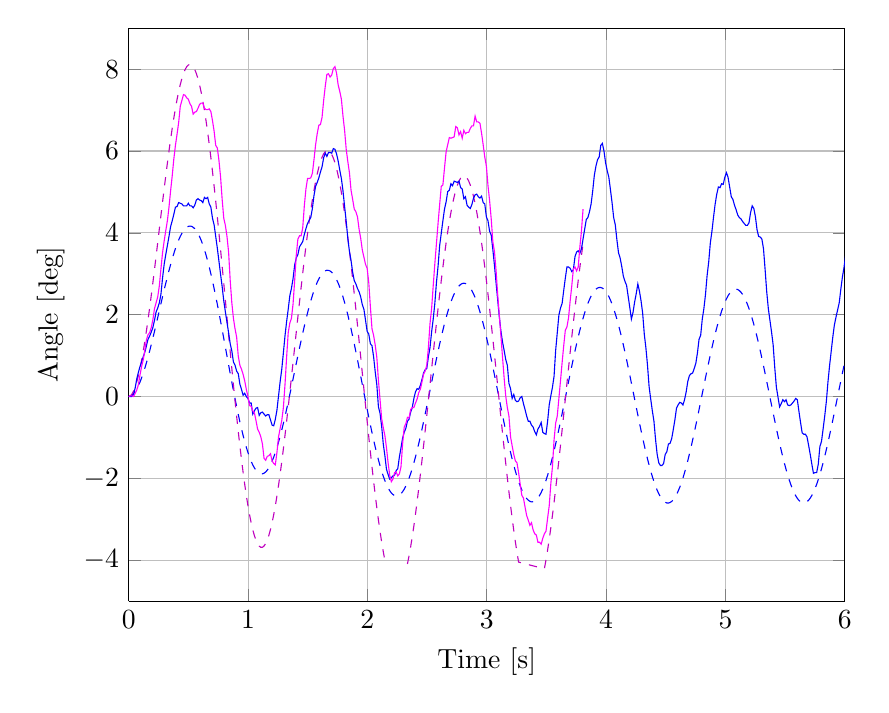
\begin{tikzpicture}

\begin{axis}[%
width=0.75\textwidth,
height=0.6\textwidth,
scale only axis,
unbounded coords=jump,
separate axis lines,
every outer x axis line/.append style={black},
every x tick label/.append style={font=\color{black}},
xmin=0,
xmax=6,
xmajorgrids,
xlabel={Time [s]},
every outer y axis line/.append style={black},
every y tick label/.append style={font=\color{black}},
ymin=-5,
ymax=9,
ymajorgrids,
ylabel={Angle [deg]},
axis background/.style={fill=white},
legend style={at={(0.97,0.97)},anchor=north east,legend cell align=left,align=left,fill=white}
]
\addplot [color=blue,dashed]
  table[row sep=crcr]{%
0	0\\
0.0135000135000135	0.00757153224291999\\
0.027000027000027	0.0300936229953074\\
0.0405000405000405	0.0672180290109261\\
0.054000054000054	0.118518770096525\\
0.0675000675000675	0.183494456976458\\
0.081000081000081	0.261571038058119\\
0.0945000945000945	0.35210494978008\\
0.108000108000108	0.454386652987249\\
0.121500121500122	0.567644535637614\\
0.135000135000135	0.691049160114935\\
0.148500148500149	0.823717831512553\\
0.162000162000162	0.964719461475604\\
0.175500175500176	1.11307970055248\\
0.189000189000189	1.26778631052027\\
0.202500202500203	1.42779474682126\\
0.216000216000216	1.59203392008624\\
0.22950022950023	1.75941210473084\\
0.243000243000243	1.92882296179994\\
0.256500256500257	2.09915164260616\\
0.27000027000027	2.26928093926474\\
0.283500283500284	2.43809744797262\\
0.297000297000297	2.60449771081343\\
0.310500310500311	2.76739430199486\\
0.324000324000324	2.92572182473844\\
0.337500337500338	3.0784427855426\\
0.351000351000351	3.22455331322596\\
0.364500364500365	3.36308869102386\\
0.378000378000378	3.49312867105398\\
0.391500391500392	3.61380254167907\\
0.405000405000405	3.7242939196713\\
0.418500418500419	3.82384524061386\\
0.432000432000432	3.91176192265507\\
0.445500445500446	3.98741618054633\\
0.459000459000459	4.05025046884034\\
0.472500472500473	4.09978053518735\\
0.486000486000486	4.135598066834\\
0.4995004995005	4.15737291569016\\
0.513000513000513	4.16485488967011\\
0.526500526500527	4.15787510042396\\
0.54000054000054	4.13634686003862\\
0.553500553500553	4.10026612179244\\
0.567000567000567	4.04971146257892\\
0.580500580500581	3.98484360715919\\
0.594000594000594	3.9059044969461\\
0.607500607500608	3.81321590855038\\
0.621000621000621	3.70717762981739\\
0.634500634500635	3.58826520353832\\
0.648000648000648	3.45702725141743\\
0.661500661500662	3.31408239320507\\
0.675000675000675	3.16011577815078\\
0.688500688500689	2.99587524808031\\
0.702000702000702	2.82216715344189\\
0.715500715500716	2.63985184559026\\
0.729000729000729	2.44983887037062\\
0.742500742500743	2.25308188971849\\
0.756000756000756	2.05057335949776\\
0.76950076950077	1.84333899314733\\
0.783000783000783	1.63243204189175\\
0.796500796500797	1.41892742328468\\
0.81000081000081	1.20391573069105\\
0.823500823500824	0.988497156969956\\
0.837000837000837	0.773775366091579\\
0.850500850500851	0.560851346705493\\
0.864000864000864	0.350817281772799\\
0.877500877500878	0.144750468280456\\
0.891000891000891	-0.0562926792268585\\
0.904500904500905	-0.251282508032182\\
0.918000918000918	-0.439221856938552\\
0.931500931500932	-0.619151604493326\\
0.945000945000945	-0.79015600498161\\
0.958500958500959	-0.951367782608294\\
0.972000972000972	-1.1019729556347\\
0.985500985500986	-1.24121536373877\\
0.999000999000999	-1.36840087351892\\
1.01250101250101	-1.48290123885158\\
1.02600102600103	-1.58415759473178\\
1.03950103950104	-1.67168356526318\\
1.05300105300105	-1.74506796860875\\
1.06650106650107	-1.80397710395238\\
1.08000108000108	-1.84815660784414\\
1.09350109350109	-1.87743286969355\\
1.10700110700111	-1.89171399862375\\
1.12050112050112	-1.89099033639038\\
1.13400113400113	-1.87533451358943\\
1.14750114750115	-1.84490104891334\\
1.16100116100116	-1.79992549375096\\
1.17450117450117	-1.74072312695003\\
1.18800118800119	-1.66768720705664\\
1.2015012015012	-1.58128679180136\\
1.21500121500122	-1.48206413700194\\
1.22850122850123	-1.37063168938497\\
1.24200124200124	-1.24766869008067\\
1.25550125550126	-1.1139174077032\\
1.26900126900127	-0.970179021981824\\
1.28250128250128	-0.817309180844994\\
1.2960012960013	-0.656213255667838\\
1.30950130950131	-0.487841321065598\\
1.32300132300132	-0.313182887140107\\
1.33650133650134	-0.133261413456289\\
1.35000135000135	0.0508713647673333\\
1.36350136350136	0.238141266732432\\
1.37700137700138	0.427457620014735\\
1.39050139050139	0.617719305330983\\
1.4040014040014	0.807820858552977\\
1.41750141750142	0.996658596089981\\
1.43100143100143	1.18313672963615\\
1.44450144450144	1.36617343634378\\
1.45800145800146	1.54470685073563\\
1.47150147150147	1.71770094510912\\
1.48500148500149	1.88415126580883\\
1.4985014985015	2.04309049354895\\
1.51200151200151	2.19359379694836\\
1.52550152550153	2.33478394959347\\
1.53900153900154	2.46583618226104\\
1.55250155250155	2.58598274340714\\
1.56600156600157	2.69451714265182\\
1.57950157950158	2.79079805375223\\
1.59300159300159	2.87425285545045\\
1.60650160650161	2.94438079059539\\
1.62000162000162	3.00075572605972\\
1.63350163350163	3.04302849819124\\
1.64700164700165	3.07092883084059\\
1.66050166050166	3.08426681538166\\
1.67400167400167	3.08293394457365\\
1.68750168750169	3.0669036945912\\
1.7010017010017	3.03623165205781\\
1.71450171450171	2.99105518544342\\
1.72800172800173	2.93159266271628\\
1.74150174150174	2.85814221965718\\
1.75500175500176	2.77108008573748\\
1.76850176850177	2.67085847691711\\
1.78200178200178	2.55800306712095\\
1.7955017955018	2.43311005248861\\
1.80900180900181	2.2968428247511\\
1.82250182250182	2.14992827225453\\
1.83600183600184	1.99315272921509\\
1.84950184950185	1.82735759573904\\
1.86300186300186	1.65343465296512\\
1.87650187650188	1.47232109937563\\
1.89000189000189	1.28499433586604\\
1.9035019035019	1.09246652855326\\
1.91700191700192	0.895778979532295\\
1.93050193050193	0.695996336852029\\
1.94400194400194	0.494200675869108\\
1.95750195750196	0.291485484847595\\
1.97100197100197	0.0889495881988978\\
1.98450198450198	-0.11230895890248\\
1.998001998002	-0.311198970637912\\
2.01150201150201	-0.506642191543165\\
2.02500202500203	-0.697579284753431\\
2.03850203850204	-0.882975714270629\\
2.05200205200205	-1.06182748862189\\
2.06550206550207	-1.23316673405229\\
2.07900207900208	-1.39606706634569\\
2.09250209250209	-1.54964873149\\
2.10600210600211	-1.69308348669026\\
2.11950211950212	-1.82559919467861\\
2.13300213300213	-1.9464841058653\\
2.14650214650215	-2.05509080461134\\
2.16000216000216	-2.15083979777111\\
2.17350217350217	-2.23322272564186\\
2.18700218700219	-2.30180517755601\\
2.2005022005022	-2.35622909654867\\
2.21400221400221	-2.39621475981638\\
2.22750222750223	-2.42156232403905\\
2.24100224100224	-2.43215292705399\\
2.25450225450225	-2.42794933983473\\
2.26800226800227	-2.4089961652237\\
2.28150228150228	-2.37541958238443\\
2.2950022950023	-2.32742663846014\\
2.30850230850231	-2.26530409143865\\
2.32200232200232	-2.18941681071384\\
2.33550233550234	-2.10020574428759\\
2.34900234900235	-1.99818546396038\\
2.36250236250236	-1.88394130219909\\
2.37600237600238	-1.75812609663476\\
2.38950238950239	-1.62145656031856\\
2.4030024030024	-1.47470929793858\\
2.41650241650242	-1.318716490162\\
2.43000243000243	-1.15436127010595\\
2.44350244350244	-0.982572817645543\\
2.45700245700246	-0.804321198829654\\
2.47050247050247	-0.620611979085899\\
2.48400248400248	-0.432480640147312\\
2.4975024975025	-0.240986831718222\\
2.51100251100251	-0.047208489809453\\
2.52450252450252	0.147764145591829\\
2.53800253800254	0.342834580298411\\
2.55150255150255	0.536906149556911\\
2.56500256500257	0.728888101767758\\
2.57850257850258	0.917701648524356\\
2.59200259200259	1.10228594739652\\
2.60550260550261	1.28160398426155\\
2.61900261900262	1.45464832254874\\
2.63250263250263	1.62044668750691\\
2.64600264600265	1.7780673545245\\
2.65950265950266	1.92662431162453\\
2.67300267300267	2.06528216751405\\
2.68650268650269	2.19326077798468\\
2.7000027000027	2.30983956502767\\
2.71350271350271	2.41436150473662\\
2.72700272700273	2.5062367619128\\
2.74050274050274	2.58494595125196\\
2.75400275400275	2.65004300706753\\
2.76750276750277	2.70115764568009\\
2.78100278100278	2.73799740686651\\
2.79450279450279	2.7603492631003\\
2.80800280800281	2.76808078771542\\
2.82150282150282	2.76114087557508\\
2.83500283500284	2.73956001231192\\
2.84850284850285	2.70345009071182\\
2.86200286200286	2.65300377532768\\
2.87550287550288	2.58849341891627\\
2.88900288900289	2.51026953677885\\
2.9025029025029	2.41875884753849\\
2.91600291600292	2.31446189129255\\
2.92950292950293	2.19795023842277\\
2.94300294300294	2.06986330461519\\
2.95650295650296	1.93090478982575\\
2.97000297000297	1.78183876101173\\
2.98350298350298	1.62348540042362\\
2.997002997003	1.4567164431048\\
3.01050301050301	1.28245032896816\\
3.02400302400302	1.10164709639878\\
3.03750303750304	0.91530304576281\\
3.05100305100305	0.724445202475208\\
3.06450306450306	0.5301256103873\\
3.07800307800308	0.333415487192168\\
3.09150309150309	0.135399274307098\\
3.10500310500311	-0.0628313857269008\\
3.11850311850312	-0.260183710891078\\
3.13200313200313	-0.45556984673127\\
3.14550314550315	-0.647912905122499\\
3.15900315900316	-0.836152941243683\\
3.17250317250317	-1.01925283559829\\
3.18600318600319	-1.19620404844869\\
3.1995031995032	-1.36603221474495\\
3.21300321300321	-1.52780254851891\\
3.22650322650323	-1.68062502677646\\
3.24000324000324	-1.82365932414926\\
3.25350325350325	-1.95611947095481\\
3.26700326700327	-2.07727820885291\\
3.28050328050328	-2.18647101996902\\
3.29400329400329	-2.28309980717051\\
3.30750330750331	-2.36663620512203\\
3.32100332100332	-2.43662450379772\\
3.33450333450333	-2.4926841682823\\
3.34800334800335	-2.5345119409359\\
3.36150336150336	-2.56188351431749\\
3.37500337500338	-2.57465476564617\\
3.38850338850339	-2.57276254601429\\
3.4020034020034	-2.5562250200386\\
3.41550341550342	-2.52514155413171\\
3.42900342900343	-2.47969215408142\\
3.44250344250344	-2.42013645512696\\
3.45600345600346	-2.34681227020435\\
3.46950346950347	-2.26013370448479\\
3.48300348300348	-2.16058884673547\\
3.4965034965035	-2.04873705038\\
3.51000351000351	-1.9252058194103\\
3.52350352350352	-1.79068731649347\\
3.53700353700354	-1.64593451271068\\
3.55050355050355	-1.49175700035203\\
3.56400356400356	-1.32901649205765\\
3.57750357750358	-1.15862203133301\\
3.59100359100359	-0.981524941064633\\
3.6045036045036	-0.798713538112398\\
3.61800361800362	-0.611207643348975\\
3.63150363150363	-0.420052917647741\\
3.64500364500365	-0.226315055282092\\
3.65850365850366	-0.0310738669857213\\
3.67200367200367	0.164582714468944\\
3.68550368550369	0.359564672891793\\
3.6990036990037	0.5527859579729\\
3.71250371250371	0.743170511680231\\
3.72600372600373	0.929658238312375\\
3.73950373950374	1.11121088507914\\
3.75300375300375	1.28681780058446\\
3.76650376650377	1.45550153926848\\
3.78000378000378	1.6163232807256\\
3.79350379350379	1.76838803384719\\
3.80700380700381	1.91084959693656\\
3.82050382050382	2.04291524630244\\
3.83400383400383	2.1638501273484\\
3.84750384750385	2.27298132383063\\
3.86100386100386	2.36970158274657\\
3.87450387450387	2.45347267423121\\
3.88800388800389	2.52382836786738\\
3.9015039015039	2.58037700894729\\
3.91500391500392	2.62280368044626\\
3.92850392850393	2.65087193877052\\
3.94200394200394	2.66442511370859\\
3.95550395550396	2.66338716543602\\
3.96900396900397	2.64776309388282\\
3.98250398250398	2.6176388982579\\
3.996003996004	2.57318108702218\\
4.00950400950401	2.514635741097\\
4.02300402300402	2.44232713557361\\
4.03650403650404	2.3566559276394\\
4.05000405000405	2.25809692084276\\
4.06350406350406	2.14719641816854\\
4.07700407700408	2.02456917867634\\
4.09050409050409	1.89089499465201\\
4.1040041040041	1.7469149083266\\
4.11750411750412	1.59342708921436\\
4.13100413100413	1.43128239500218\\
4.14450414450415	1.26137964067579\\
4.15800415800416	1.08466060218347\\
4.17150417150417	0.902104782407877\\
4.18500418500419	0.714723968531329\\
4.1985041985042	0.523556611033687\\
4.21200421200421	0.329662055547217\\
4.22550422550423	0.134114659605019\\
4.23900423900424	-0.0620021730464148\\
4.25250425250425	-0.257602007447195\\
4.26600426600427	-0.451601408344553\\
4.27950427950428	-0.642925953558444\\
4.29300429300429	-0.830516196419207\\
4.30650430650431	-1.01333354419193\\
4.32000432000432	-1.19036601987333\\
4.33350433350433	-1.36063387539921\\
4.34700434700435	-1.52319502512992\\
4.36050436050436	-1.67715026948353\\
4.37400437400437	-1.82164827975551\\
4.38750438750439	-1.95589031649354\\
4.4010044010044	-2.07913465527919\\
4.41450441450441	-2.19070069539572\\
4.42800442800443	-2.28997272862537\\
4.44150444150444	-2.37640334730895\\
4.45500445500446	-2.44951647280607\\
4.46850446850447	-2.50890998760381\\
4.48200448200448	-2.55425795652423\\
4.4955044955045	-2.58531242476362\\
4.50900450900451	-2.60190478284722\\
4.52250452250452	-2.603946690988\\
4.53600453600454	-2.59143055778496\\
4.54950454950455	-2.56442957067046\\
4.56300456300456	-2.52309727800449\\
4.57650457650458	-2.46766672520228\\
4.59000459000459	-2.39844914975642\\
4.6035046035046	-2.31583224246246\\
4.61700461700462	-2.22027798456307\\
4.63050463050463	-2.11232007287868\\
4.64400464400464	-1.99256094727717\\
4.65750465750466	-1.86166843704027\\
4.67100467100467	-1.72037204479699\\
4.68450468450468	-1.56945888870347\\
4.6980046980047	-1.40976932544199\\
4.71150471150471	-1.2421922783804\\
4.72500472500473	-1.06766029686583\\
4.73850473850474	-0.887144374115069\\
4.75200475200475	-0.701648552499601\\
4.76550476550477	-0.512204346199228\\
4.77900477900478	-0.319865012207165\\
4.79250479250479	-0.125699701506732\\
4.80600480600481	0.0692124770999807\\
4.81950481950482	0.263788447551107\\
4.83300483300483	0.456947178214356\\
4.84650484650485	0.647615681337073\\
4.86000486000486	0.834734966960291\\
4.87350487350487	1.01726591825773\\
4.88700488700489	1.19419505570175\\
4.9005049005049	1.36454015808021\\
4.91400491400491	1.52735570918733\\
4.92750492750493	1.68173813998399\\
4.94100494100494	1.82683083716261\\
4.95450495450496	1.96182889035241\\
4.96800496800497	2.08598355165584\\
4.98150498150498	2.19860638280746\\
4.995004995005	2.29907306698374\\
5.00850500850501	2.38682686415753\\
5.02200502200502	2.46138169087188\\
5.03550503550504	2.52232480739568\\
5.04900504900505	2.56931909740526\\
5.06250506250506	2.60210492759973\\
5.07600507600508	2.62050157699121\\
5.08950508950509	2.6244082280013\\
5.1030051030051	2.61380451392805\\
5.11650511650512	2.58875061981087\\
5.13000513000513	2.54938693620035\\
5.14350514350514	2.49593326782088\\
5.15700515700516	2.42868760158477\\
5.17050517050517	2.34802444086123\\
5.18400518400518	2.25439271531003\\
5.1975051975052	2.14831327794406\\
5.21100521100521	2.03037600337423\\
5.22450522450522	1.90123650340156\\
5.23800523800524	1.76161247824273\\
5.25150525150525	1.61227972369516\\
5.26500526500527	1.4540678164539\\
5.27850527850528	1.28785550157602\\
5.29200529200529	1.1145658077376\\
5.30550530550531	0.935160917435342\\
5.31900531900532	0.750636820641192\\
5.33250533250533	0.562017781615562\\
5.34600534600535	0.370350649617789\\
5.35950535950536	0.176699045113988\\
5.37300537300537	-0.0178625462311107\\
5.38650538650539	-0.21225473898474\\
5.4000054000054	-0.405399239680607\\
5.41350541350541	-0.596224831597748\\
5.42700542700543	-0.78367331936774\\
5.44050544050544	-0.966705400422173\\
5.45400545400545	-1.14430643070326\\
5.46750546750547	-1.3154920526522\\
5.48100548100548	-1.47931365425902\\
5.49450549450549	-1.63486362890002\\
5.50800550800551	-1.78128040679904\\
5.52150552150552	-1.91775323022068\\
5.53500553500554	-2.0435266459302\\
5.54850554850555	-2.15790469002789\\
5.56200556200556	-2.26025474197687\\
5.57550557550558	-2.35001102648286\\
5.58900558900559	-2.42667774384198\\
5.6025056025056	-2.48983181143784\\
5.61600561600562	-2.5391252012298\\
5.62950562950563	-2.57428686031899\\
5.64300564300564	-2.59512420399468\\
5.65650565650566	-2.6015241730378\\
5.67000567000567	-2.59345384947836\\
5.68350568350568	-2.57096062745502\\
5.6970056970057	-2.5341719382947\\
5.71050571050571	-2.48329453140467\\
5.72400572400572	-2.41861331503449\\
5.73750573750574	-2.3404897634076\\
5.75100575100575	-2.24935989912787\\
5.76450576450577	-2.14573186212277\\
5.77800577800578	-2.03018307867764\\
5.79150579150579	-1.90335704633339\\
5.80500580500581	-1.76595975254944\\
5.81850581850582	-1.61875574706396\\
5.83200583200583	-1.46256388980231\\
5.84550584550585	-1.29825279798242\\
5.85900585900586	-1.12673601773157\\
5.87250587250587	-0.94896694705447\\
5.88600588600589	-0.765933538368588\\
5.8995058995059	-0.578652810041806\\
5.91300591300591	-0.388165197423353\\
5.92650592650593	-0.195528774745148\\
5.94000594000594	-0.00181337998275785\\
5.95350595350595	0.191905324700991\\
5.96700596700597	0.384551823954082\\
5.98050598050598	0.575056718529758\\
5.99400599400599	0.762362659746468\\
6.00750600750601	0.945430216180702\\
6.02100602100602	1.12324364004113\\
6.03450603450603	1.2948165012341\\
6.04800604800605	1.45919715786976\\
6.06150606150606	1.61547403287026\\
6.07500607500608	1.76278066742263\\
6.08850608850609	1.90030052326132\\
6.1020061020061	2.02727150716424\\
6.11550611550612	2.14299019259117\\
6.12900612900613	2.24681571507888\\
6.14250614250614	2.3381733198208\\
6.15600615600616	2.41655754179325\\
6.16950616950617	2.48153500083241\\
6.18300618300618	2.53274679620596\\
6.1965061965062	2.56991048744865\\
6.21000621000621	2.59282165052925\\
6.22350622350622	2.60135500077501\\
6.23700623700624	2.59546507638574\\
6.25050625050625	2.57518647880914\\
6.26400626400626	2.54063366870952\\
6.27750627750628	2.49200031872828\\
6.29100629100629	2.42955822669475\\
6.3045063045063	2.35365579538471\\
6.31800631800632	2.26471608732895\\
6.33150633150633	2.16323446553158\\
6.34500634500635	2.04977583325426\\
6.35850635850636	1.92497148824613\\
6.37200637200637	1.78951560893669\\
6.38550638550639	1.64416139214901\\
6.3990063990064	1.48971686382176\\
6.41250641250641	1.32704038604068\\
6.42600642600643	1.15703588536143\\
6.43950643950644	0.980647828949801\\
6.45300645300645	0.798855976460287\\
6.46650646650647	0.612669936815051\\
6.48000648000648	0.423123560123509\\
6.49350649350649	0.231269195893459\\
6.50700650700651	0.0381718494220564\\
6.52050652050652	-0.155096731184648\\
6.53400653400653	-0.347464004534713\\
6.54750654750655	-0.53786258898903\\
6.56100656100656	-0.725236186174332\\
6.57450657450658	-0.90854544209788\\
6.58800658800659	-1.08677371334244\\
6.6015066015066	-1.2589327063518\\
6.61500661500662	-1.42406795852632\\
6.62850662850663	-1.58126413073047\\
6.64200664200664	-1.7296500818659\\
6.65550665550666	-1.8684036973771\\
6.66900666900667	-1.99675644492703\\
6.68250668250668	-2.11399763199816\\
6.6960066960067	-2.21947834183255\\
6.70950670950671	-2.31261502591345\\
6.72300672300672	-2.39289273310043\\
6.73650673650674	-2.4598679575496\\
6.75000675000675	-2.51317108966907\\
6.76350676350676	-2.55250845656548\\
6.77700677700678	-2.57766394071756\\
6.79050679050679	-2.58850016795579\\
6.8040068040068	-2.5849592582185\\
6.81750681750682	-2.56706313498291\\
6.83100683100683	-2.53491339171933\\
6.84450684450684	-2.48869071617576\\
6.85800685800686	-2.42865387575422\\
6.87150687150687	-2.35513826967564\\
6.88500688500689	-2.26855405603368\\
6.8985068985069	-2.16938386419626\\
6.91200691200691	-2.05818010531324\\
6.92550692550693	-1.9355618959177\\
6.93900693900694	-1.80221161175312\\
6.95250695250695	-1.65887109100888\\
6.96600696600697	-1.50633750808915\\
6.97950697950698	-1.34545894086622\\
6.99300699300699	-1.17712965606653\\
7.00650700650701	-1.00228513899901\\
7.02000702000702	-0.821896895249894\\
7.03350703350703	-0.636967053230116\\
7.04700704700705	-0.448522797562146\\
7.06050706050706	-0.257610664227612\\
7.07400707400707	-0.0652907291597676\\
7.08750708750709	0.127369277448542\\
7.1010071010071	0.319299898443194\\
7.11450711450712	0.509435885709156\\
7.12800712800713	0.696722111925273\\
7.14150714150714	0.880119425265304\\
7.15500715500716	1.0586104145586\\
7.16850716850717	1.23120505292566\\
7.18200718200718	1.39694618858299\\
7.1955071955072	1.55491485236468\\
7.20900720900721	1.70423535252991\\
7.22250722250722	1.84408012861052\\
7.23600723600724	1.97367433739451\\
7.24950724950725	2.09230014563197\\
7.26300726300726	2.19930070568147\\
7.27650727650728	2.29408379207836\\
7.29000729000729	2.37612507889159\\
7.3035073035073	2.4449710397324\\
7.31700731700732	2.50024145437524\\
7.33050733050733	2.54163150813734\\
7.34400734400734	2.5689134724253\\
7.35750735750736	2.58193795718377\\
7.37100737100737	2.5806347283586\\
7.38450738450739	2.56501308590213\\
7.3980073980074	2.535161800288\\
7.41150741150741	2.49124860795382\\
7.42500742500743	2.43351926853764\\
7.43850743850744	2.36229618920629\\
7.45200745200745	2.2779766237753\\
7.46550746550747	2.18103045667915\\
7.47900747900748	2.07199758415333\\
7.49250749250749	1.95148490722326\\
7.50600750600751	1.82016295324761\\
7.51950751950752	1.67876214482274\\
7.53300753300753	1.52806873680935\\
7.54650754650755	1.36892044408126\\
7.56000756000756	1.20220178430966\\
7.57350757350757	1.02883916167393\\
7.58700758700759	0.849795718824396\\
7.6005076005076	0.666065985704488\\
7.61400761400761	0.478670354962898\\
7.62750762750763	0.288649414644597\\
7.64100764100764	0.0970581696369277\\
7.65450765450765	-0.0950398160401584\\
7.66800766800767	-0.28657832357613\\
7.68150768150768	-0.476494397566587\\
7.6950076950077	-0.663734245215088\\
7.70850770850771	-0.847259083800808\\
7.72200772200772	-1.02605090396481\\
7.73550773550774	-1.19911811683973\\
7.74900774900775	-1.36550105369715\\
7.76250776250776	-1.52427728761023\\
7.77600777600778	-1.67456674762143\\
7.78950778950779	-1.81553659706137\\
7.8030078030078	-1.94640584897806\\
7.81650781650782	-2.06644969309876\\
7.83000783000783	-2.17500351035182\\
7.84350784350784	-2.27146655271332\\
7.85700785700786	-2.35530526800437\\
7.87050787050787	-2.42605625123853\\
7.88400788400788	-2.48332880619411\\
7.8975078975079	-2.52680710305222\\
7.91100791100791	-2.55625192018523\\
7.92450792450793	-2.57150196049026\\
7.93800793800794	-2.57247473502514\\
7.95150795150795	-2.55916700910688\\
7.96500796500797	-2.53165480846189\\
7.97850797850798	-2.49009298545943\\
7.99200799200799	-2.43471434790139\\
8.00550800550801	-2.36582835526884\\
8.01900801900802	-2.28381938972632\\
8.03250803250803	-2.18914461154328\\
8.04600804600805	-2.0823314108978\\
8.05950805950806	-1.96397447026574\\
8.07300807300807	-1.83473245375801\\
8.08650808650809	-1.69532434183646\\
8.1000081000081	-1.54652543180454\\
8.11350811350811	-1.38916302632087\\
8.12700812700813	-1.2241118339122\\
8.14050814050814	-1.05228910705668\\
8.15400815400815	-0.87464954486192\\
8.16750816750817	-0.692179988663929\\
8.18100818100818	-0.505893940018912\\
8.1945081945082	-0.316825931540783\\
8.20800820800821	-0.126025781849712\\
8.22150822150822	0.0654472334645429\\
8.23500823500824	0.256530262499311\\
8.24850824850825	0.446162776668851\\
8.26200826200826	0.633292456560057\\
8.27550827550828	0.816881031348051\\
8.28900828900829	0.995910039368326\\
8.3025083025083	1.16938647788452\\
8.31600831600832	1.33634831071065\\
8.32950832950833	1.49586980314031\\
8.34300834300834	1.64706665459822\\
8.35650835650836	1.78910090055688\\
8.37000837000837	1.92118555654571\\
8.38350838350839	2.04258897851562\\
8.3970083970084	2.15263891540029\\
8.41050841050841	2.25072623142709\\
8.42400842400843	2.33630827756717\\
8.43750843750844	2.40891189346459\\
8.45100845100845	2.468136023238\\
8.46450846450847	2.51365393069411\\
8.47800847800848	2.54521500171768\\
8.49150849150849	2.56264612389561\\
8.50500850500851	2.56585263578117\\
8.51850851850852	2.5548188405936\\
8.53200853200853	2.52960808156692\\
8.54550854550855	2.49036237859508\\
8.55900855900856	2.43730162825551\\
8.57250857250857	2.37072237171626\\
8.58600858600859	2.29099613742944\\
8.5995085995086	2.19856736787303\\
8.61300861300861	2.09395094190992\\
8.62650862650863	1.97772930657615\\
8.64000864000864	1.85054923427585\\
8.65350865350865	1.71311822343703\\
8.66700866700867	1.56620056265877\\
8.68050868050868	1.41061308024485\\
8.69400869400869	1.24722060276192\\
8.70750870750871	1.07693114787184\\
8.72100872100872	0.900690878158623\\
8.73450873450873	0.719478843993407\\
8.74800874800875	0.534301544647111\\
8.76150876150876	0.346187337865273\\
8.77500877500878	0.156180728955865\\
8.78850878850879	-0.0346634288948925\\
8.8020088020088	-0.225285790875746\\
8.81550881550882	-0.414628400860508\\
8.82900882900883	-0.601640563134202\\
8.84250884250884	-0.785284672946958\\
8.85600885600886	-0.964541973540689\\
8.86950886950887	-1.13841820770654\\
8.88300888300888	-1.30594913252119\\
8.8965088965089	-1.46620586667429\\
8.91000891000891	-1.61830004073273\\
8.92350892350892	-1.76138872178605\\
8.93700893700894	-1.8946790851734\\
8.95050895050895	-2.01743280740048\\
8.96400896400896	-2.12897015590627\\
8.97750897750898	-2.2286737530253\\
8.99100899100899	-2.31599199330326\\
9.00450900450901	-2.39044209525046\\
9.01800901800902	-2.45161277064965\\
9.03150903150903	-2.49916649665987\\
9.04500904500905	-2.53284137816479\\
9.05850905850906	-2.55245259008995\\
9.07200907200907	-2.5578933917465\\
9.08550908550909	-2.54913570763504\\
9.0990090990091	-2.52623027155092\\
9.11250911250911	-2.48930633325592\\
9.12600912600913	-2.43857092940977\\
9.13950913950914	-2.37430772287293\\
9.15300915300915	-2.29687541688701\\
9.16650916650917	-2.20670575299804\\
9.18000918000918	-2.10430110389657\\
9.1935091935092	-1.99023167459543\\
9.20700920700921	-1.86513232753753\\
9.22050922050922	-1.72969904931146\\
9.23400923400924	-1.58468507863872\\
9.24750924750925	-1.43089671717382\\
9.26100926100926	-1.26918884641579\\
9.27450927450928	-1.10046017565692\\
9.28800928800929	-0.925648247384162\\
9.3015093015093	-0.74572422789061\\
9.31500931500932	-0.56168751204241\\
9.32850932850933	-0.374560172173857\\
9.34200934200934	-0.185381281943929\\
9.35550935550936	0.00479885332305619\\
9.36900936900937	0.194924527775598\\
9.38250938250938	0.383940495278512\\
9.3960093960094	0.570797826231564\\
9.40950940950941	0.754459728456888\\
9.42300942300942	0.933907299853119\\
9.43650943650944	1.10814518089769\\
9.45000945000945	1.27620707563936\\
9.46350946350946	1.43716111055764\\
9.47700947700948	1.59011500157027\\
9.49050949050949	1.73422100053899\\
9.5040095040095	1.86868059385223\\
9.51750951750952	1.99274892704322\\
9.53100953100953	2.10573893092658\\
9.54450954450954	2.20702512639683\\
9.55800955800956	2.29604708681895\\
9.57150957150957	2.37231253884501\\
9.58500958500959	2.43540008450028\\
9.5985095985096	2.48496152948712\\
9.61200961200961	2.52072380484254\\
9.62550962550963	2.54249047134435\\
9.63900963900964	2.55014279837827\\
9.65250965250965	2.54364041134146\\
9.66600966600967	2.52302150405342\\
9.67950967950968	2.48840261506019\\
9.69300969300969	2.43997796913847\\
9.70650970650971	2.3780183877192\\
9.72000972000972	2.30286977434231\\
9.73350973350973	2.21495118361209\\
9.74700974700975	2.11475248443304\\
9.76050976050976	2.0028316305563\\
9.77400977400977	1.8798115536444\\
9.78750978750979	1.74637669615478\\
9.8010098010098	1.60326920333933\\
9.81450981450982	1.45128479554588\\
};
%\addlegendentry{1A model};

\addplot [color=mycolor1,dashed] 
  table[row sep=crcr]{%
0	0\\
0.0135000135000135	0.014754202999143\\
0.027000027000027	0.0586416868352673\\
0.0405000405000405	0.130983850218277\\
0.054000054000054	0.23095061040624\\
0.0675000675000675	0.357564939379311\\
0.081000081000081	0.509708216301237\\
0.0945000945000945	0.686126366418915\\
0.108000108000108	0.885436752190276\\
0.121500121500122	1.10613577826114\\
0.135000135000135	1.34660716795561\\
0.148500148500149	1.60513086522407\\
0.162000162000162	1.87989251252871\\
0.175500175500176	2.16899345195725\\
0.189000189000189	2.47046119395999\\
0.202500202500203	2.78226029551804\\
0.216000216000216	3.10230358728753\\
0.22950022950023	3.42846368733644\\
0.243000243000243	3.75858473751009\\
0.256500256500257	4.09049429723508\\
0.27000027000027	4.42201532870785\\
0.283500283500284	4.75097820691677\\
0.297000297000297	5.0752326878192\\
0.310500310500311	5.392659768237\\
0.324000324000324	5.70118337164562\\
0.337500337500338	5.99878179500778\\
0.351000351000351	6.2834988531393\\
0.364500364500365	6.5534546587828\\
0.378000378000378	6.80685597859662\\
0.391500391500392	7.04200610762894\\
0.405000405000405	7.25731420752863\\
0.418500418500419	7.45130405672896\\
0.432000432000432	7.62262216411205\\
0.445500445500446	7.77004520120217\\
0.459000459000459	7.89248671172515\\
0.472500472500473	7.98900306138847\\
0.486000486000486	8.05879859495925\\
0.4995004995005	8.10122997212202\\
0.513000513000513	8.11580965816084\\
0.526500526500527	8.10220855020475\\
0.54000054000054	8.06025772457673\\
0.553500553500553	7.98994929566647\\
0.567000567000567	7.89143638168049\\
0.580500580500581	7.76503217758076\\
0.594000594000594	7.61120814047854\\
0.607500607500608	7.43059129767592\\
0.621000621000621	7.22396069241511\\
0.634500634500635	6.99224298718013\\
0.648000648000648	6.73650724906794\\
0.661500661500662	6.45795894628272\\
0.675000675000675	6.15793318918104\\
0.688500688500689	5.83788725348389\\
0.702000702000702	5.49939242725024\\
0.715500715500716	5.1441252269541\\
0.729000729000729	4.77385803150191\\
0.742500742500743	4.39044918625075\\
0.756000756000756	3.99583263202177\\
0.76950076950077	3.59200711673163\\
0.783000783000783	3.18102504957278\\
0.796500796500797	2.76498105964869\\
0.81000081000081	2.34600032260143\\
0.823500823500824	1.92622672004708\\
0.837000837000837	1.50781089755336\\
0.850500850500851	1.09289828744681\\
0.864000864000864	0.683617162922795\\
0.877500877500878	0.282066789747596\\
0.891000891000891	-0.109694258709041\\
0.904500904500905	-0.489659558289195\\
0.918000918000918	-0.855885999163726\\
0.931500931500932	-1.20650459733322\\
0.945000945000945	-1.53973089256694\\
0.958500958500959	-1.85387487513809\\
0.972000972000972	-2.14735038633735\\
0.985500985500986	-2.41868394067545\\
0.999000999000999	-2.66652292090307\\
1.01250101250101	-2.88964310046433\\
1.02600102600103	-3.08695545173997\\
1.03950103950104	-3.25751220240623\\
1.05300105300105	-3.4005121064143\\
1.06650106650107	-3.51530490045895\\
1.08000108000108	-3.60139492133021\\
1.09350109350109	-3.65844386420252\\
1.10700110700111	-3.686272666687\\
1.12050112050112	-3.68486250832653\\
1.13400113400113	-3.65435492012471\\
1.14750114750115	-3.59505100363962\\
1.16100116100116	-3.5074097641157\\
1.17450117450117	-3.39204556704351\\
1.18800118800119	-3.24972473240084\\
1.2015012015012	-3.08136128561256\\
1.21500121500122	-2.88801188894407\\
1.22850122850123	-2.67086998158846\\
1.24200124200124	-2.43125916109496\\
1.25550125550126	-2.17062584299237\\
1.26900126900127	-1.89053123946145\\
1.28250128250128	-1.59264270168383\\
1.2960012960013	-1.2787244740198\\
1.30950130950131	-0.950627911424718\\
1.32300132300132	-0.61028121448517\\
1.33650133650134	-0.259678739125141\\
1.35000135000135	0.0991300596154139\\
1.36350136350136	0.464051988305123\\
1.37700137700138	0.832961717243602\\
1.39050139050139	1.20371355954605\\
1.4040014040014	1.57415336178191\\
1.41750141750142	1.94213044015005\\
1.43100143100143	2.30550949593023\\
1.44450144450144	2.66218244407546\\
1.45800145800146	3.01008008930184\\
1.47150147150147	3.34718358488902\\
1.48500148500149	3.67153561061966\\
1.4985014985015	3.9812512078553\\
1.51200151200151	4.27452821165765\\
1.52550152550153	4.54965722211043\\
1.53900153900154	4.80503105956272\\
1.55250155250155	5.03915365138766\\
1.56600156600157	5.25064830101336\\
1.57950157950158	5.43826529341886\\
1.59300159300159	5.60088879497763\\
1.60650160650161	5.73754300945405\\
1.62000162000162	5.8473975560925\\
1.63350163350163	5.92977204006147\\
1.64700164700165	5.98413979000231\\
1.66050166050166	6.0101307420586\\
1.67400167400167	6.00753345450278\\
1.68750168750169	5.97629624190434\\
1.7010017010017	5.91652742267238\\
1.71450171450171	5.82849467872733\\
1.72800172800173	5.71262353098472\\
1.74150174150174	5.56949493924104\\
1.75500175500176	5.39984203990999\\
1.76850176850177	5.20454603984091\\
1.78200178200178	4.98463128913228\\
1.7955017955018	4.74125956040676\\
1.80900180900181	4.47572356641432\\
1.82250182250182	4.18943975205301\\
1.83600183600184	3.88394040091867\\
1.84950184950185	3.56086510029336\\
1.86300186300186	3.22195161203683\\
1.87650187650188	2.86902620013567\\
1.89000189000189	2.50399346867271\\
1.9035019035019	2.1288257666889\\
1.91700191700192	1.74555221880527\\
1.93050193050193	1.35624744254071\\
1.94400194400194	0.96302001499164\\
1.95750195750196	0.568000752921114\\
1.97100197100197	0.173330871331083\\
1.98450198450198	-0.218849913743557\\
1.998001998002	-0.606415272180809\\
2.01150201150201	-0.987264070485652\\
2.02500202500203	-1.35933204073366\\
2.03850203850204	-1.72060324300198\\
2.05200205200205	-2.06912125770144\\
2.06550206550207	-2.40300004573195\\
2.07900207900208	-2.72043441623629\\
2.09250209250209	-3.01971004391449\\
2.10600210600211	-3.29921298036912\\
2.11950211950212	-3.55743860676905\\
2.13300213300213	-3.79299997822719\\
2.14650214650215	-4.00463551367172\\
nan	nan\\
2.33550233550234	-4.0925483636632\\
2.34900234900235	-3.8937473974011\\
2.36250236250236	-3.67112646678707\\
2.37600237600238	-3.42595771841241\\
2.38950238950239	-3.15963776917183\\
2.4030024030024	-2.8736799432975\\
2.41650241650242	-2.56970586268863\\
2.43000243000243	-2.24943643731\\
2.44350244350244	-1.91468230575631\\
2.45700245700246	-1.56733377912291\\
2.47050247050247	-1.20935034407276\\
2.48400248400248	-0.842749783427184\\
2.4975024975025	-0.469596974722747\\
2.51100251100251	-0.0919924289542518\\
2.52450252450252	0.287939366842871\\
2.53800253800254	0.668061738438561\\
2.55150255150255	1.04623767923042\\
2.56500256500257	1.42034170523378\\
2.57850257850258	1.78827164443994\\
2.59200259200259	2.14796029511709\\
2.60550260550261	2.49738688836554\\
2.61900261900262	2.83458829133508\\
2.63250263250263	3.15766988896101\\
2.64600264600265	3.46481608386924\\
2.65950265950266	3.75430035622881\\
2.67300267300267	4.0244948277815\\
2.68650268650269	4.27387927703847\\
2.7000027000027	4.50104955568774\\
2.71350271350271	4.70472535958756\\
2.72700272700273	4.88375731130952\\
2.74050274050274	5.03713331502316\\
2.75400275400275	5.16398414855788\\
2.76750276750277	5.26358826171777\\
2.78100278100278	5.33537575433429\\
2.79450279450279	5.3789315120991\\
2.80800280800281	5.39399748289661\\
2.82150282150282	5.38047408112935\\
2.83500283500284	5.33842071237045\\
2.84850284850285	5.26805541556159\\
2.86200286200286	5.16975362487286\\
2.87550287550288	5.04404605822662\\
2.88900288900289	4.89161574433399\\
2.9025029025029	4.71329420487197\\
2.91600291600292	4.51005681311627\\
2.92950292950293	4.2830173549123\\
2.94300294300294	4.03342182229049\\
2.95650295650296	3.7626414742863\\
2.97000297000297	3.47216520358763\\
2.98350298350298	3.16359125147928\\
2.997002997003	2.83861831716496\\
3.01050301050301	2.49903611090175\\
3.02400302400302	2.14671540346181\\
3.03750303750304	1.78359762722351\\
3.05100305100305	1.41168408667469\\
3.06450306450306	1.03302483827004\\
3.07800307800308	0.649707301410669\\
3.09150309150309	0.263844663797292\\
3.10500310500311	-0.122435854459842\\
3.11850311850312	-0.507004812816705\\
3.13200313200313	-0.88774237278681\\
3.14550314550315	-1.26255006532934\\
3.15900315900316	-1.62936243783096\\
3.17250317250317	-1.98615851605616\\
3.18600318600319	-2.33097301747767\\
3.1995031995032	-2.66190725378767\\
3.21300321300321	-2.9771396621251\\
3.22650322650323	-3.27493590662401\\
3.24000324000324	-3.55365849428141\\
3.25350325350325	-3.81177585184701\\
3.26700326700327	-4.04787081343688\\
3.48300348300348	-4.21021339138162\\
3.4965034965035	-3.99225432361292\\
3.51000351000351	-3.75153622323565\\
3.52350352350352	-3.48940786724382\\
3.53700353700354	-3.20733652643913\\
3.55050355050355	-2.90689980606864\\
3.56400356400356	-2.58977687526368\\
3.57750357750358	-2.25773913405064\\
3.59100359100359	-1.91264036981827\\
3.6045036045036	-1.55640645795221\\
3.61800361800362	-1.1910246638692\\
3.63150363150363	-0.818532605887307\\
3.64500364500365	-0.441006940242062\\
3.65850365850366	-0.0605518310913101\\
3.67200367200367	0.320712730464225\\
3.68550368550369	0.700662693489375\\
3.6990036990037	1.07718173512823\\
3.71250371250371	1.44817300389366\\
3.72600372600373	1.81157075316062\\
3.73950373950374	2.1653518003104\\
3.75300375300375	2.50754674795017\\
3.76650376650377	2.83625090496219\\
3.78000378000378	3.14963484681264\\
3.79350379350379	3.44595455656075\\
3.80700380700381	3.72356109034541\\
};
%\addlegendentry{3A model};

\addplot [color=blue,solid]
  table[row sep=crcr]{%
0	9.99999999993229e-05\\
0.0135000135000135	9.99999999993229e-05\\
0.027000027000027	9.99999999993229e-05\\
0.0405000405000405	0.0477999999999983\\
0.054000054000054	0.206800000000001\\
0.0675000675000675	0.429400000000001\\
0.081000081000081	0.5884\\
0.0945000945000945	0.7315\\
0.108000108000108	0.8428\\
0.121500121500122	0.969999999999998\\
0.135000135000135	1.0813\\
0.148500148500149	1.2403\\
0.162000162000162	1.3993\\
0.175500175500176	1.4788\\
0.189000189000189	1.5742\\
0.202500202500203	1.6855\\
0.216000216000216	1.8604\\
0.22950022950023	2.0671\\
0.243000243000243	2.1625\\
0.256500256500257	2.2897\\
0.27000027000027	2.4964\\
0.283500283500284	2.8939\\
0.297000297000297	3.2278\\
0.310500310500311	3.4663\\
0.324000324000324	3.6889\\
0.337500337500338	3.9115\\
0.351000351000351	4.15\\
0.364500364500364	4.2931\\
0.378000378000378	4.4521\\
0.391500391500392	4.627\\
0.405000405000405	4.6429\\
0.418500418500419	4.7383\\
0.432000432000432	4.7224\\
0.445500445500446	4.7065\\
0.459000459000459	4.6588\\
0.472500472500473	4.6588\\
0.486000486000486	4.6588\\
0.4995004995005	4.7224\\
0.513000513000513	4.6588\\
0.526500526500526	4.6588\\
0.54000054000054	4.6111\\
0.553500553500553	4.6747\\
0.567000567000567	4.8019\\
0.580500580500581	4.8337\\
0.594000594000594	4.8019\\
0.607500607500608	4.786\\
0.621000621000621	4.7383\\
0.634500634500635	4.8655\\
0.648000648000648	4.8337\\
0.661500661500662	4.8655\\
0.675000675000675	4.7065\\
0.688500688500689	4.627\\
0.702000702000702	4.3567\\
0.715500715500716	4.1977\\
0.729000729000729	3.9115\\
0.742500742500742	3.6253\\
0.756000756000756	3.3073\\
0.76950076950077	2.9893\\
0.783000783000783	2.6872\\
0.796500796500797	2.3374\\
0.81000081000081	2.0671\\
0.823500823500824	1.8127\\
0.837000837000837	1.5583\\
0.850500850500851	1.288\\
0.864000864000864	1.1131\\
0.877500877500878	0.8428\\
0.891000891000891	0.763300000000001\\
0.904500904500905	0.6202\\
0.918000918000918	0.556599999999999\\
0.931500931500931	0.302199999999999\\
0.945000945000945	0.175\\
0.958500958500959	0.0318999999999998\\
0.972000972000972	0.0795999999999988\\
0.985500985500986	9.99999999993229e-05\\
0.999000999000999	-0.0475999999999996\\
1.01250101250101	-0.1589\\
1.02600102600103	-0.1589\\
1.03950103950104	-0.429200000000002\\
1.05300105300105	-0.349700000000003\\
1.06650106650107	-0.286100000000002\\
1.08000108000108	-0.2702\\
1.09350109350109	-0.461000000000003\\
1.10700110700111	-0.397400000000002\\
1.12050112050112	-0.3815\\
1.13400113400113	-0.429200000000002\\
1.14750114750115	-0.476900000000001\\
1.16100116100116	-0.445100000000001\\
1.17450117450117	-0.445100000000001\\
1.18800118800119	-0.572300000000002\\
1.2015012015012	-0.699500000000001\\
1.21500121500122	-0.715399999999999\\
1.22850122850123	-0.5564\\
1.24200124200124	-0.333800000000001\\
1.25550125550126	0.0159999999999978\\
1.26900126900127	0.3658\\
1.28250128250128	0.667899999999999\\
1.2960012960013	1.0654\\
1.30950130950131	1.4788\\
1.32300132300132	1.8286\\
1.33650133650134	2.1307\\
1.35000135000135	2.4646\\
1.36350136350136	2.6395\\
1.37700137700138	2.878\\
1.39050139050139	3.2119\\
1.4040014040014	3.3868\\
1.41750141750142	3.4663\\
1.43100143100143	3.6571\\
1.44450144450144	3.7207\\
1.45800145800146	3.7843\\
1.47150147150147	3.9592\\
1.48500148500149	4.1023\\
1.4985014985015	4.2295\\
1.51200151200151	4.309\\
1.52550152550153	4.3726\\
1.53900153900154	4.5952\\
1.55250155250155	4.9132\\
1.56600156600157	5.1358\\
1.57950157950158	5.2312\\
1.59300159300159	5.3425\\
1.60650160650161	5.4856\\
1.62000162000162	5.6128\\
1.63350163350163	5.8354\\
1.64700164700165	5.9467\\
1.66050166050166	5.8672\\
1.67400167400167	5.9626\\
1.68750168750169	5.9626\\
1.7010017010017	5.9467\\
1.71450171450171	6.058\\
1.72800172800173	6.0421\\
1.74150174150174	5.9308\\
1.75500175500176	5.7559\\
1.76850176850177	5.5333\\
1.78200178200178	5.3266\\
1.7955017955018	5.0245\\
1.80900180900181	4.6429\\
1.82250182250182	4.2772\\
1.83600183600184	3.8638\\
1.84950184950185	3.5458\\
1.86300186300186	3.3232\\
1.87650187650188	3.037\\
1.89000189000189	2.8303\\
1.9035019035019	2.7508\\
1.91700191700192	2.6395\\
1.93050193050193	2.56\\
1.94400194400194	2.4328\\
1.95750195750196	2.242\\
1.97100197100197	2.1307\\
1.98450198450198	1.8604\\
1.998001998002	1.5901\\
2.01150201150201	1.5265\\
2.02500202500203	1.288\\
2.03850203850204	1.2403\\
2.05200205200205	0.969999999999998\\
2.06550206550207	0.604299999999998\\
2.07900207900208	0.2863\\
2.09250209250209	-0.254300000000001\\
2.10600210600211	-0.4133\\
2.11950211950212	-0.731300000000001\\
2.13300213300213	-1.1606\\
2.14650214650215	-1.4468\\
2.16000216000216	-1.7807\\
2.17350217350217	-1.9079\\
2.18700218700219	-2.0192\\
2.2005022005022	-1.9874\\
2.21400221400221	-1.9397\\
2.22750222750223	-1.9238\\
2.24100224100224	-1.8125\\
2.25450225450225	-1.7648\\
2.26800226800227	-1.4786\\
2.28150228150228	-1.256\\
2.2950022950023	-1.0175\\
2.30850230850231	-0.874400000000002\\
2.32200232200232	-0.779\\
2.33550233550234	-0.604099999999999\\
2.34900234900235	-0.5564\\
2.36250236250236	-0.3815\\
2.37600237600238	-0.2702\\
2.38950238950239	-0.0475999999999996\\
2.4030024030024	0.111399999999999\\
2.41650241650242	0.190899999999999\\
2.43000243000243	0.175\\
2.44350244350244	0.270399999999998\\
2.45700245700246	0.413499999999999\\
2.47050247050247	0.572499999999998\\
2.48400248400248	0.652000000000001\\
2.4975024975025	0.683799999999998\\
2.51100251100251	0.969999999999998\\
2.52450252450252	1.1926\\
2.53800253800254	1.5742\\
2.55150255150255	1.8922\\
2.56500256500257	2.2738\\
2.57850257850258	2.7826\\
2.59200259200259	3.1801\\
2.60550260550261	3.6889\\
2.61900261900262	3.991\\
2.63250263250263	4.2931\\
2.64600264600265	4.5793\\
2.65950265950266	4.7542\\
2.67300267300267	5.0086\\
2.68650268650269	5.0404\\
2.7000027000027	5.1994\\
2.71350271350271	5.1517\\
2.72700272700273	5.263\\
2.74050274050274	5.2471\\
2.75400275400275	5.2312\\
2.76750276750277	5.263\\
2.78100278100278	5.104\\
2.79450279450279	5.0722\\
2.80800280800281	4.8337\\
2.82150282150282	4.8814\\
2.83500283500284	4.6747\\
2.84850284850285	4.627\\
2.86200286200286	4.5952\\
2.87550287550288	4.6906\\
2.88900288900289	4.8496\\
2.9025029025029	4.9291\\
2.91600291600292	4.945\\
2.92950292950293	4.8814\\
2.94300294300294	4.8496\\
2.95650295650296	4.8973\\
2.97000297000297	4.7383\\
2.98350298350298	4.7065\\
2.997002997003	4.3885\\
3.01050301050301	4.2931\\
3.02400302400302	4.0387\\
3.03750303750304	3.9433\\
3.05100305100305	3.5935\\
3.06450306450306	3.2119\\
3.07800307800308	2.7826\\
3.09150309150309	2.3692\\
3.10500310500311	1.9558\\
3.11850311850312	1.606\\
3.13200313200313	1.3357\\
3.14550314550315	1.129\\
3.15900315900316	0.906399999999997\\
3.17250317250317	0.763300000000001\\
3.18600318600319	0.318100000000001\\
3.1995031995032	0.190899999999999\\
3.21300321300321	-0.0475999999999996\\
3.22650322650323	0.0477999999999983\\
3.24000324000324	-0.0953000000000022\\
3.25350325350325	-0.127100000000003\\
3.26700326700327	-0.111200000000001\\
3.28050328050328	-0.0317000000000012\\
3.29400329400329	9.99999999993229e-05\\
3.30750330750331	-0.174800000000002\\
3.32100332100332	-0.317900000000002\\
3.33450333450333	-0.476900000000001\\
3.34800334800335	-0.604099999999999\\
3.36150336150336	-0.604099999999999\\
3.37500337500338	-0.699500000000001\\
3.38850338850339	-0.7472\\
3.4020034020034	-0.8585\\
3.41550341550342	-0.938000000000003\\
3.42900342900343	-0.794900000000002\\
3.44250344250344	-0.731300000000001\\
3.45600345600346	-0.6359\\
3.46950346950347	-0.874400000000002\\
3.48300348300348	-0.906200000000002\\
3.4965034965035	-0.922100000000001\\
3.51000351000351	-0.604099999999999\\
3.52350352350352	-0.206600000000002\\
3.53700353700354	0.0159999999999978\\
3.55050355050355	0.222699999999999\\
3.56400356400356	0.492999999999998\\
3.57750357750358	1.129\\
3.59100359100359	1.5583\\
3.6045036045036	1.9876\\
3.61800361800362	2.1625\\
3.63150363150363	2.2738\\
3.64500364500365	2.5918\\
3.65850365850366	2.8939\\
3.67200367200367	3.1642\\
3.68550368550369	3.1642\\
3.6990036990037	3.1324\\
3.71250371250371	3.0529\\
3.72600372600373	3.1006\\
3.73950373950374	3.4186\\
3.75300375300375	3.5299\\
3.76650376650377	3.5617\\
3.78000378000378	3.4981\\
3.79350379350379	3.6094\\
3.80700380700381	3.8479\\
3.82050382050382	4.0864\\
3.83400383400383	4.3249\\
3.84750384750385	4.3726\\
3.86100386100386	4.5157\\
3.87450387450387	4.7065\\
3.88800388800389	5.0245\\
3.9015039015039	5.4061\\
3.91500391500392	5.6287\\
3.92850392850393	5.7877\\
3.94200394200394	5.8513\\
3.95550395550396	6.1375\\
3.96900396900397	6.1852\\
3.98250398250398	5.9944\\
3.996003996004	5.7082\\
4.00950400950401	5.5174\\
4.02300402300402	5.3584\\
4.03650403650404	5.0563\\
4.05000405000405	4.7383\\
4.06350406350406	4.3726\\
4.07700407700408	4.1977\\
4.09050409050409	3.832\\
4.1040041040041	3.514\\
4.11750411750412	3.3868\\
4.13100413100413	3.1801\\
4.14450414450415	2.9416\\
4.15800415800416	2.8144\\
4.17150417150417	2.719\\
4.18500418500419	2.4487\\
4.1985041985042	2.1784\\
4.21200421200421	1.8922\\
4.22550422550423	2.0512\\
4.23900423900424	2.3056\\
4.25250425250425	2.5123\\
4.26600426600427	2.7508\\
4.27950427950428	2.5759\\
4.29300429300429	2.3374\\
4.30650430650431	2.0353\\
4.32000432000432	1.5265\\
4.33350433350433	1.1926\\
4.34700434700435	0.763300000000001\\
4.36050436050436	0.238599999999998\\
4.37400437400437	-0.0635000000000017\\
4.38750438750439	-0.349700000000003\\
4.4010044010044	-0.604099999999999\\
4.41450441450441	-1.0493\\
4.42800442800443	-1.415\\
4.44150444150444	-1.6217\\
4.45500445500446	-1.6853\\
4.46850446850447	-1.6853\\
4.48200448200448	-1.6376\\
4.4955044955045	-1.415\\
4.50900450900451	-1.3514\\
4.52250452250452	-1.1606\\
4.53600453600454	-1.1447\\
4.54950454950455	-1.0334\\
4.56300456300456	-0.810800000000001\\
4.57650457650458	-0.572300000000002\\
4.59000459000459	-0.286100000000002\\
4.6035046035046	-0.206600000000002\\
4.61700461700462	-0.143000000000001\\
4.63050463050463	-0.1589\\
4.64400464400464	-0.206600000000002\\
4.65750465750466	-0.0794000000000001\\
4.67100467100467	0.111399999999999\\
4.68450468450468	0.3658\\
4.6980046980047	0.5089\\
4.71150471150471	0.556599999999999\\
4.72500472500472	0.572499999999998\\
4.73850473850474	0.683799999999998\\
4.75200475200475	0.811\\
4.76550476550477	1.0654\\
4.77900477900478	1.3993\\
4.79250479250479	1.4947\\
4.80600480600481	1.8922\\
4.81950481950482	2.1466\\
4.83300483300483	2.4964\\
4.84650484650485	2.9575\\
4.86000486000486	3.2914\\
4.87350487350487	3.7525\\
4.88700488700489	4.0387\\
4.9005049005049	4.3885\\
4.91400491400491	4.7065\\
4.92750492750493	4.945\\
4.94100494100494	5.1199\\
4.95450495450496	5.104\\
4.96800496800497	5.1994\\
4.98150498150498	5.1835\\
4.995004995005	5.3584\\
5.00850500850501	5.4697\\
5.02200502200502	5.3584\\
5.03550503550504	5.1199\\
5.04900504900505	4.8814\\
5.06250506250506	4.8178\\
5.07600507600508	4.6747\\
5.08950508950509	4.5634\\
5.1030051030051	4.4362\\
5.11650511650512	4.3726\\
5.13000513000513	4.3408\\
5.14350514350514	4.2772\\
5.15700515700516	4.2295\\
5.17050517050517	4.1818\\
5.18400518400518	4.1818\\
5.1975051975052	4.2454\\
5.21100521100521	4.4998\\
5.22450522450522	4.6588\\
5.23800523800524	4.5952\\
5.25150525150525	4.3885\\
5.26500526500527	4.0705\\
5.27850527850528	3.9115\\
5.29200529200529	3.8956\\
5.30550530550531	3.8479\\
5.31900531900532	3.6094\\
5.33250533250533	3.1006\\
5.34600534600535	2.56\\
5.35950535950536	2.1466\\
5.37300537300537	1.8604\\
5.38650538650539	1.5742\\
5.4000054000054	1.2562\\
5.41350541350541	0.6997\\
5.42700542700543	0.222699999999999\\
5.44050544050544	-0.0158000000000027\\
5.45400545400545	-0.254300000000001\\
5.46750546750547	-0.174800000000002\\
5.48100548100548	-0.0794000000000001\\
5.49450549450549	-0.127100000000003\\
5.50800550800551	-0.0794000000000001\\
5.52150552150552	-0.206600000000002\\
5.53500553500553	-0.222500000000001\\
5.54850554850555	-0.206600000000002\\
5.56200556200556	-0.1589\\
5.57550557550558	-0.111200000000001\\
5.58900558900559	-0.0475999999999996\\
5.6025056025056	-0.0794000000000001\\
5.61600561600562	-0.365600000000001\\
5.62950562950563	-0.6359\\
5.64300564300564	-0.8903\\
5.65650565650566	-0.922100000000001\\
5.67000567000567	-0.922100000000001\\
5.68350568350568	-0.985700000000002\\
5.6970056970057	-1.1924\\
5.71050571050571	-1.415\\
5.72400572400572	-1.6535\\
5.73750573750574	-1.8761\\
5.75100575100575	-1.8602\\
5.76450576450577	-1.8602\\
5.77800577800578	-1.6535\\
5.79150579150579	-1.2242\\
5.80500580500581	-1.097\\
5.81850581850582	-0.794900000000002\\
5.83200583200583	-0.476900000000001\\
5.84550584550585	-0.127100000000003\\
5.85900585900586	0.349899999999998\\
5.87250587250587	0.747399999999999\\
5.88600588600589	1.0972\\
5.8995058995059	1.447\\
5.91300591300591	1.7491\\
5.92650592650593	1.9399\\
5.94000594000594	2.1148\\
5.95350595350595	2.2897\\
5.96700596700597	2.6236\\
5.98050598050598	2.9257\\
5.99400599400599	3.1642\\
6.00750600750601	3.4504\\
6.02100602100602	3.3391\\
6.03450603450603	3.2119\\
6.04800604800605	3.196\\
6.06150606150606	3.196\\
6.07500607500608	3.4186\\
6.08850608850609	3.514\\
6.1020061020061	3.6253\\
6.11550611550612	3.8161\\
6.12900612900613	4.0546\\
6.14250614250614	4.3249\\
6.15600615600616	4.627\\
6.16950616950617	5.0245\\
6.18300618300618	5.2471\\
6.1965061965062	5.422\\
6.21000621000621	5.4856\\
6.22350622350622	5.5969\\
6.23700623700624	5.8195\\
6.25050625050625	5.899\\
6.26400626400626	5.9149\\
6.27750627750628	5.7241\\
6.29100629100629	5.5174\\
6.3045063045063	5.1994\\
6.31800631800632	4.9927\\
6.33150633150633	4.7224\\
6.34500634500635	4.4362\\
6.35850635850636	4.0705\\
6.37200637200637	3.5617\\
6.38550638550639	3.2755\\
6.3990063990064	2.9098\\
6.41250641250641	2.7349\\
6.42600642600643	2.5441\\
6.43950643950644	2.3215\\
6.45300645300645	2.3692\\
6.46650646650647	2.2738\\
6.48000648000648	2.3374\\
6.49350649350649	2.3374\\
6.50700650700651	2.242\\
6.52050652050652	2.0989\\
6.53400653400653	1.8604\\
6.54750654750655	1.765\\
6.56100656100656	1.5742\\
6.57450657450658	1.4311\\
6.58800658800659	1.2403\\
6.6015066015066	0.922299999999999\\
6.61500661500662	0.652000000000001\\
6.62850662850663	0.302199999999999\\
6.64200664200664	0.0477999999999983\\
6.65550665550666	-0.445100000000001\\
6.66900666900667	-0.763100000000002\\
6.68250668250668	-1.1606\\
6.6960066960067	-1.4945\\
6.70950670950671	-1.6694\\
6.72300672300672	-1.9556\\
6.73650673650674	-2.0828\\
6.75000675000675	-2.2736\\
6.76350676350676	-2.2895\\
6.77700677700678	-2.0033\\
6.79050679050679	-1.7648\\
6.8040068040068	-1.4468\\
6.81750681750682	-1.3355\\
6.83100683100683	-1.2401\\
6.84450684450684	-1.2242\\
6.85800685800686	-1.1924\\
6.87150687150687	-0.906200000000002\\
6.88500688500689	-0.6677\\
6.8985068985069	-0.365600000000001\\
6.91200691200691	-0.174800000000002\\
6.92550692550693	-0.222500000000001\\
6.93900693900694	-0.174800000000002\\
6.95250695250695	-0.143000000000001\\
6.96600696600697	-0.0475999999999996\\
6.97950697950698	9.99999999993229e-05\\
6.99300699300699	9.99999999993229e-05\\
7.00650700650701	9.99999999993229e-05\\
7.02000702000702	-0.0158000000000027\\
7.03350703350703	0.2545\\
7.04700704700705	0.413499999999999\\
7.06050706050706	0.667899999999999\\
7.07400707400707	0.779199999999999\\
7.08750708750709	1.0813\\
7.1010071010071	1.4629\\
7.11450711450711	1.9399\\
7.12800712800713	2.3851\\
7.14150714150714	2.719\\
7.15500715500716	2.8144\\
7.16850716850717	3.0211\\
7.18200718200718	3.4345\\
7.1955071955072	4.0069\\
7.20900720900721	4.468\\
7.22250722250722	4.8337\\
7.23600723600724	4.9609\\
7.24950724950725	5.104\\
7.26300726300726	5.2153\\
7.27650727650728	5.3425\\
7.29000729000729	5.3743\\
7.3035073035073	5.3584\\
7.31700731700732	5.2471\\
7.33050733050733	5.1835\\
7.34400734400734	4.9768\\
7.35750735750736	4.945\\
7.37100737100737	4.6747\\
7.38450738450739	4.5157\\
7.3980073980074	4.3885\\
7.41150741150741	4.3726\\
7.42500742500743	4.3726\\
7.43850743850744	4.4044\\
7.45200745200745	4.4044\\
7.46550746550747	4.4203\\
7.47900747900748	4.4521\\
7.49250749250749	4.5157\\
7.50600750600751	4.5952\\
7.51950751950752	4.7224\\
7.53300753300753	4.5793\\
7.54650754650755	4.2613\\
7.56000756000756	3.8956\\
7.57350757350757	3.6094\\
7.58700758700759	3.4504\\
7.6005076005076	3.0529\\
7.61400761400761	2.5759\\
7.62750762750763	2.0512\\
7.64100764100764	1.5265\\
7.65450765450765	1.288\\
7.66800766800767	0.938199999999998\\
7.68150768150768	0.6202\\
7.6950076950077	0.206800000000001\\
7.70850770850771	-0.302\\
7.72200772200772	-0.476900000000001\\
7.73550773550774	-0.699500000000001\\
7.74900774900775	-0.5564\\
7.76250776250776	-0.874400000000002\\
7.77600777600778	-0.9698\\
7.78950778950779	-1.1924\\
7.8030078030078	-1.256\\
7.81650781650782	-0.985700000000002\\
7.83000783000783	-1.1288\\
7.84350784350784	-1.0493\\
7.85700785700786	-1.3196\\
7.87050787050787	-1.415\\
7.88400788400788	-1.3196\\
7.8975078975079	-1.3832\\
7.91100791100791	-1.1606\\
7.92450792450792	-1.6058\\
7.93800793800794	-1.7807\\
7.95150795150795	-1.9397\\
7.96500796500797	-1.8761\\
7.97850797850798	-1.6853\\
7.99200799200799	-2.0033\\
8.00550800550801	-1.9238\\
8.01900801900802	-2.2736\\
8.03250803250803	-2.1464\\
8.04600804600805	-2.051\\
8.05950805950806	-2.0351\\
8.07300807300807	-1.5899\\
8.08650808650809	-1.7012\\
8.1000081000081	-1.2401\\
8.11350811350811	-1.2242\\
8.12700812700813	-0.5246\\
8.14050814050814	0.270399999999998\\
8.15400815400815	0.492999999999998\\
8.16750816750817	1.2085\\
8.18100818100818	0.922299999999999\\
8.1945081945082	1.3516\\
8.20800820800821	1.6219\\
8.22150822150822	2.0194\\
8.23500823500824	2.2897\\
8.24850824850825	2.1943\\
8.26200826200826	2.5441\\
8.27550827550828	2.3215\\
8.28900828900829	2.878\\
8.3025083025083	3.0847\\
8.31600831600832	3.2278\\
8.32950832950833	3.4186\\
8.34300834300834	3.2914\\
8.35650835650836	3.5458\\
8.37000837000837	3.3391\\
8.38350838350838	3.7843\\
8.3970083970084	3.9115\\
8.41050841050841	4.0864\\
8.42400842400842	4.4203\\
8.43750843750844	4.5634\\
8.45100845100845	4.9609\\
8.46450846450846	4.9291\\
8.47800847800848	5.3902\\
8.49150849150849	5.4856\\
8.50500850500851	5.6446\\
8.51850851850852	5.7082\\
8.53200853200853	5.4379\\
8.54550854550855	5.581\\
8.55900855900856	5.4379\\
8.57250857250857	5.5492\\
8.58600858600859	5.3266\\
8.5995085995086	5.1517\\
8.61300861300861	4.786\\
8.62650862650863	4.468\\
8.64000864000864	4.3726\\
8.65350865350865	3.9433\\
8.66700866700867	3.7684\\
8.68050868050868	3.3232\\
8.69400869400869	3.1801\\
8.70750870750871	2.878\\
8.72100872100872	2.6077\\
8.73450873450873	2.6872\\
8.74800874800875	2.3692\\
8.76150876150876	2.3056\\
8.77500877500878	2.0353\\
8.78850878850879	1.9717\\
8.8020088020088	1.765\\
8.81550881550882	1.606\\
8.82900882900883	1.4788\\
8.84250884250884	1.129\\
8.85600885600886	1.0972\\
8.86950886950887	0.7315\\
8.88300888300888	0.636099999999999\\
8.8965088965089	0.318100000000001\\
8.91000891000891	0.0159999999999978\\
8.92350892350892	-0.254300000000001\\
8.93700893700894	-0.620000000000001\\
8.95050895050895	-0.810800000000001\\
8.96400896400896	-1.256\\
8.97750897750898	-1.4945\\
8.99100899100899	-1.7648\\
9.00450900450901	-1.9397\\
9.01800901800902	-2.0669\\
9.03150903150903	-2.21\\
9.04500904500905	-2.2418\\
9.05850905850906	-2.3213\\
9.07200907200907	-2.2418\\
9.08550908550909	-2.1782\\
9.0990090990091	-2.0828\\
9.11250911250911	-1.9238\\
9.12600912600913	-1.8602\\
9.13950913950914	-1.7012\\
9.15300915300915	-1.7171\\
9.16650916650917	-1.5263\\
9.18000918000918	-1.6376\\
9.19350919350919	-1.4627\\
9.20700920700921	-1.4309\\
9.22050922050922	-1.3991\\
9.23400923400923	-1.2719\\
9.24750924750925	-1.256\\
9.26100926100926	-1.0652\\
9.27450927450927	-1.1288\\
9.28800928800929	-0.953900000000001\\
9.3015093015093	-0.731300000000001\\
9.31500931500932	-0.461000000000003\\
9.32850932850933	-0.111200000000001\\
9.34200934200934	9.99999999993229e-05\\
9.35550935550936	0.3976\\
9.36900936900937	0.7315\\
9.38250938250938	1.2562\\
9.3960093960094	1.7491\\
9.40950940950941	2.1625\\
9.42300942300942	2.6872\\
9.43650943650944	2.8939\\
9.45000945000945	3.2437\\
9.46350946350946	3.5299\\
9.47700947700948	3.832\\
9.49050949050949	4.15\\
9.5040095040095	4.3567\\
9.51750951750952	4.7065\\
9.53100953100953	4.7701\\
9.54450954450954	5.0404\\
9.55800955800956	5.1517\\
9.57150957150957	5.1835\\
9.58500958500959	5.2312\\
9.5985095985096	5.2789\\
9.61200961200961	5.3107\\
9.62550962550963	5.0722\\
9.63900963900964	5.1835\\
9.65250965250965	5.0881\\
9.66600966600967	5.0563\\
9.67950967950968	5.1358\\
9.69300969300969	5.1199\\
9.70650970650971	5.1517\\
9.72000972000972	5.1835\\
9.73350973350973	5.1994\\
9.74700974700975	5.1358\\
9.76050976050976	5.1994\\
9.77400977400977	5.0404\\
9.78750978750979	4.945\\
9.8010098010098	4.8019\\
9.81450981450982	4.4521\\
};
%\addlegendentry{1A samples};

\addplot [color=mycolor3,solid] %
  table[row sep=crcr]{%
0	-1.66533453693773e-15\\
0.0135000135000135	0.0159000000000004\\
0.027000027000027	0.0159000000000004\\
0.0405000405000405	-1.66533453693773e-15\\
0.054000054000054	0.0794999999999978\\
0.0675000675000675	0.158999999999997\\
0.081000081000081	0.286199999999999\\
0.0945000945000945	0.524699999999998\\
0.108000108000108	0.731399999999999\\
0.121500121500122	0.890399999999998\\
0.135000135000135	1.1289\\
0.148500148500149	1.3833\\
0.162000162000162	1.5105\\
0.175500175500176	1.5582\\
0.189000189000189	1.6854\\
0.202500202500203	1.8762\\
0.216000216000216	2.1465\\
0.22950022950023	2.2896\\
0.243000243000243	2.4327\\
0.256500256500257	2.703\\
0.27000027000027	3.1164\\
0.283500283500284	3.5139\\
0.297000297000297	3.8001\\
0.310500310500311	4.0545\\
0.324000324000324	4.293\\
0.337500337500338	4.6269\\
0.351000351000351	5.0244\\
0.364500364500364	5.3901\\
0.378000378000378	5.8035\\
0.391500391500392	6.1374\\
0.405000405000405	6.4077\\
0.418500418500419	6.6939\\
0.432000432000432	7.0914\\
0.445500445500446	7.2345\\
0.459000459000459	7.3776\\
0.472500472500473	7.3617\\
0.486000486000486	7.2981\\
0.4995004995005	7.2663\\
0.513000513000513	7.155\\
0.526500526500526	7.0914\\
0.54000054000054	6.9006\\
0.553500553500553	6.9483\\
0.567000567000567	6.9642\\
0.580500580500581	7.0437\\
0.594000594000594	7.1391\\
0.607500607500608	7.1709\\
0.621000621000621	7.1709\\
0.634500634500635	7.0437\\
0.648000648000648	7.0119\\
0.661500661500662	7.0119\\
0.675000675000675	7.0278\\
0.688500688500689	6.9642\\
0.702000702000702	6.7416\\
0.715500715500716	6.4872\\
0.729000729000729	6.1374\\
0.742500742500742	6.0738\\
0.756000756000756	5.7717\\
0.76950076950077	5.3742\\
0.783000783000783	4.8177\\
0.796500796500797	4.3566\\
0.81000081000081	4.1817\\
0.823500823500824	3.9114\\
0.837000837000837	3.5298\\
0.850500850500851	2.8302\\
0.864000864000864	2.2896\\
0.877500877500878	1.908\\
0.891000891000891	1.6536\\
0.904500904500905	1.4469\\
0.918000918000918	0.985799999999999\\
0.931500931500931	0.7632\\
0.945000945000945	0.667799999999998\\
0.958500958500959	0.5406\\
0.972000972000972	0.381599999999997\\
0.985500985500986	0.174899999999999\\
0.999000999000999	-1.66533453693773e-15\\
1.01250101250101	-0.222600000000002\\
1.02600102600103	-0.2385\\
1.03950103950104	-0.3498\\
1.05300105300105	-0.397500000000003\\
1.06650106650107	-0.588300000000002\\
1.08000108000108	-0.795\\
1.09350109350109	-0.874500000000003\\
1.10700110700111	-0.985800000000003\\
1.12050112050112	-1.1607\\
1.13400113400113	-1.5105\\
1.14750114750115	-1.5582\\
1.16100116100116	-1.4628\\
1.17450117450117	-1.4469\\
1.18800118800119	-1.3992\\
1.2015012015012	-1.5741\\
1.21500121500122	-1.6377\\
1.22850122850123	-1.6695\\
1.24200124200124	-1.3674\\
1.25550125550126	-0.985800000000003\\
1.26900126900127	-0.779100000000001\\
1.28250128250128	-0.588300000000002\\
1.2960012960013	-0.270300000000001\\
1.30950130950131	0.286199999999999\\
1.32300132300132	0.953999999999999\\
1.33650133650134	1.5582\\
1.35000135000135	1.7967\\
1.36350136350136	1.908\\
1.37700137700138	2.2578\\
1.39050139050139	2.8302\\
1.4040014040014	3.4503\\
1.41750141750142	3.8478\\
1.43100143100143	3.9273\\
1.44450144450144	3.9273\\
1.45800145800146	4.1181\\
1.47150147150147	4.6587\\
1.48500148500149	5.0721\\
1.4985014985015	5.3265\\
1.51200151200151	5.3265\\
1.52550152550153	5.3424\\
1.53900153900154	5.4537\\
1.55250155250155	5.7876\\
1.56600156600157	6.1533\\
1.57950157950158	6.4236\\
1.59300159300159	6.6303\\
1.60650160650161	6.6462\\
1.62000162000162	6.8211\\
1.63350163350163	7.2345\\
1.64700164700165	7.5843\\
1.66050166050166	7.8705\\
1.67400167400167	7.8864\\
1.68750168750169	7.8069\\
1.7010017010017	7.8546\\
1.71450171450171	8.0136\\
1.72800172800173	8.0613\\
1.74150174150174	7.9023\\
1.75500175500176	7.6161\\
1.76850176850177	7.4571\\
1.78200178200178	7.2663\\
1.7955017955018	6.8529\\
1.80900180900181	6.5031\\
1.82250182250182	6.042\\
1.83600183600184	5.7399\\
1.84950184950185	5.4696\\
1.86300186300186	5.0403\\
1.87650187650188	4.8177\\
1.89000189000189	4.5792\\
1.9035019035019	4.5156\\
1.91700191700192	4.3884\\
1.93050193050193	4.0863\\
1.94400194400194	3.8637\\
1.95750195750196	3.5775\\
1.97100197100197	3.4026\\
1.98450198450198	3.2277\\
1.998001998002	3.1323\\
2.01150201150201	2.7825\\
2.02500202500203	2.1942\\
2.03850203850204	1.6536\\
2.05200205200205	1.4946\\
2.06550206550207	1.2561\\
2.07900207900208	0.953999999999999\\
2.09250209250209	0.397499999999999\\
2.10600210600211	-0.0795000000000011\\
2.11950211950212	-0.540599999999999\\
2.13300213300213	-0.763200000000003\\
2.14650214650215	-0.954000000000002\\
2.16000216000216	-1.2561\\
2.17350217350217	-1.6218\\
2.18700218700219	-1.9239\\
2.2005022005022	-2.0829\\
2.21400221400221	-2.0193\\
2.22750222750223	-1.8603\\
2.24100224100224	-1.8444\\
2.25450225450225	-1.9398\\
2.26800226800227	-1.8921\\
2.28150228150228	-1.7172\\
2.2950022950023	-1.1607\\
2.30850230850231	-0.747300000000001\\
2.32200232200232	-0.667800000000001\\
2.33550233550234	-0.508800000000002\\
2.34900234900235	-0.524700000000001\\
2.36250236250236	-0.318\\
2.37600237600238	-0.270300000000001\\
2.38950238950239	-0.270300000000001\\
2.4030024030024	-0.159000000000001\\
2.41650241650242	-0.0636000000000027\\
2.43000243000243	0.0953999999999998\\
2.44350244350244	0.174899999999999\\
2.45700245700246	0.3498\\
2.47050247050247	0.5406\\
2.48400248400248	0.620099999999999\\
2.4975024975025	0.7632\\
2.51100251100251	1.1925\\
2.52450252450252	1.7808\\
2.53800253800254	2.1465\\
2.55150255150255	2.703\\
2.56500256500257	3.2436\\
2.57850257850258	3.7365\\
2.59200259200259	4.2294\\
2.60550260550261	4.6905\\
2.61900261900262	5.1357\\
2.63250263250263	5.1675\\
2.64600264600265	5.5809\\
2.65950265950266	5.9784\\
2.67300267300267	6.1533\\
2.68650268650269	6.3282\\
2.7000027000027	6.3123\\
2.71350271350271	6.3282\\
2.72700272700273	6.3441\\
2.74050274050274	6.5985\\
2.75400275400275	6.5667\\
2.76750276750277	6.3918\\
2.78100278100278	6.4713\\
2.79450279450279	6.3123\\
2.80800280800281	6.5031\\
2.82150282150282	6.4236\\
2.83500283500284	6.4554\\
2.84850284850285	6.4554\\
2.86200286200286	6.5508\\
2.87550287550288	6.6144\\
2.88900288900289	6.6144\\
2.9025029025029	6.8529\\
2.91600291600292	6.7098\\
2.92950292950293	6.7098\\
2.94300294300294	6.678\\
2.95650295650296	6.4395\\
2.97000297000297	6.1533\\
2.98350298350298	5.8512\\
2.997002997003	5.6286\\
3.01050301050301	5.1516\\
3.02400302400302	4.7859\\
3.03750303750304	4.3407\\
3.05100305100305	3.7842\\
3.06450306450306	3.5457\\
3.07800307800308	3.0846\\
3.09150309150309	2.4963\\
3.10500310500311	2.0034\\
3.11850311850312	1.4946\\
3.13200313200313	0.969899999999997\\
3.14550314550315	0.4611\\
3.15900315900316	0.0159000000000004\\
3.17250317250317	-0.270300000000001\\
3.18600318600319	-0.477000000000002\\
3.1995031995032	-0.985800000000003\\
3.21300321300321	-1.2084\\
3.22650322650323	-1.4151\\
3.24000324000324	-1.5741\\
3.25350325350325	-1.6218\\
3.26700326700327	-1.8603\\
3.28050328050328	-2.1465\\
3.29400329400329	-2.4168\\
3.30750330750331	-2.4804\\
3.32100332100332	-2.703\\
3.33450333450333	-2.9097\\
3.34800334800335	-3.021\\
3.36150336150336	-3.1482\\
3.37500337500338	-3.0846\\
3.38850338850339	-3.2595\\
3.4020034020034	-3.3549\\
3.41550341550342	-3.3867\\
3.42900342900343	-3.5616\\
3.44250344250344	-3.5616\\
3.45600345600346	-3.6093\\
3.46950346950347	-3.4662\\
3.48300348300348	-3.3549\\
3.4965034965035	-3.2913\\
3.51000351000351	-2.9733\\
3.52350352350352	-2.6712\\
3.53700353700354	-2.1306\\
3.55050355050355	-1.7172\\
3.56400356400356	-1.0653\\
3.57750357750358	-0.651899999999999\\
3.59100359100359	-0.477000000000002\\
3.6045036045036	-0.0477000000000006\\
3.61800361800362	0.381599999999997\\
3.63150363150363	0.826800000000001\\
3.64500364500365	1.2402\\
3.65850365850366	1.6218\\
3.67200367200367	1.7013\\
3.68550368550369	1.9239\\
3.6990036990037	2.3373\\
3.71250371250371	2.703\\
3.72600372600373	3.1164\\
3.73950373950374	3.1641\\
3.75300375300375	3.0687\\
3.76650376650377	3.1641\\
3.78000378000378	3.6411\\
3.79350379350379	4.0386\\
3.80700380700381	4.5792\\
};
%\addlegendentry{2A samples};


%\addlegendentry{3A samples};
\end{axis}

\begin{axis}[%
width=0.8\textwidth,
height=0.6\textwidth,
at={(1.85in,0.746in)},
scale only axis,
every outer x axis line/.append style={black},
every x tick label/.append style={font=\color{black}},
xmin=0,
xmax=1,
xlabel={Time [s]},
every outer y axis line/.append style={black},
every y tick label/.append style={font=\color{black}},
ymin=0,
ymax=1,
ylabel={Angle [deg]},
hide axis,
axis x line*=bottom,
axis y line*=left
]
\end{axis}
\end{tikzpicture}%
              \end{figure}}	     	
    \end{itemize}           
  \end{minipage}
\end{frame} 
%%%%%%%%%%%%%%%%

\begin{frame}{Model opstilling}{Trolley- og pendulmodel}
  \begin{minipage}[t]{0.48\linewidth}
    \begin{itemize}
      	\item<1->[] {
              \begin{figure}[H]
              \centering
              % This file was created by matlab2tikz.
%
%The latest updates can be retrieved from
%  http://www.mathworks.com/matlabcentral/fileexchange/22022-matlab2tikz-matlab2tikz
%where you can also make suggestions and rate matlab2tikz.
%
\definecolor{mycolor1}{rgb}{0.75000,0.00000,0.75000}%
\definecolor{mycolor2}{rgb}{1.00000,0.00000,1.00000}%
%
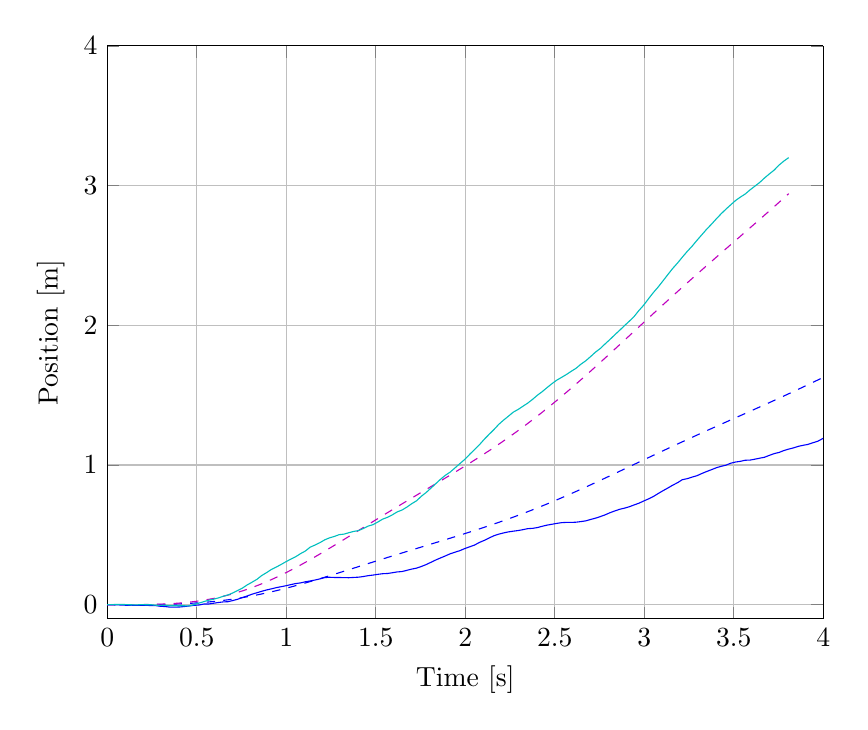
\begin{tikzpicture}

\begin{axis}[%
width=0.75\textwidth,
height=0.6\textwidth,
scale only axis,
separate axis lines,
every outer x axis line/.append style={black},
every x tick label/.append style={font=\color{black}},
xmin=0,
xmax=4,
xmajorgrids,
xlabel={Time [s]},
every outer y axis line/.append style={black},
every y tick label/.append style={font=\color{black}},
ymin=-0.1,
ymax=4,
ymajorgrids,
ylabel={Position [m]},
axis background/.style={fill=white},
legend style={at={(0.97,0.03)},anchor=south east,legend cell align=left,align=left,draw=black}
]
\addplot [color=blue,dashed]
  table[row sep=crcr]{%
0	0\\
0.027000027000027	5.69402929386811e-07\\
0.054000054000054	5.39144829692237e-06\\
0.081000081000081	2.09682892992041e-05\\
0.108000108000108	5.61415637614898e-05\\
0.135000135000135	0.00012194467512605\\
0.162000162000162	0.000231433023656061\\
0.189000189000189	0.000399494294085924\\
0.216000216000216	0.000642641099126427\\
0.243000243000243	0.000978788444094646\\
0.27000027000027	0.00142701861499061\\
0.297000297000297	0.00200733619942392\\
0.324000324000324	0.00274041602608231\\
0.351000351000351	0.00364734685345482\\
0.378000378000378	0.0047493736521451\\
0.405000405000405	0.00606764130755025\\
0.432000432000432	0.00762294252148985\\
0.459000459000459	0.009435472613428\\
0.486000486000486	0.0115245938154332\\
0.513000513000513	0.013908611521458\\
0.54000054000054	0.0166045647926638\\
0.567000567000567	0.0196280332383884\\
0.594000594000594	0.0229929621892166\\
0.621000621000621	0.0267115078569171\\
0.648000648000648	0.0307939039383957\\
0.675000675000675	0.0352483508700504\\
0.702000702000702	0.040080928677898\\
0.729000729000729	0.0452955341005251\\
0.756000756000756	0.050893842389326\\
0.783000783000783	0.0568752939166365\\
0.81000081000081	0.0632371054502627\\
0.837000837000837	0.0699743056854884\\
0.864000864000864	0.0770797943657768\\
0.891000891000891	0.0845444240738228\\
0.918000918000918	0.0923571035379509\\
0.945000945000945	0.100504921077531\\
0.972000972000972	0.108973286607332\\
0.999000999000999	0.117746090436588\\
1.02600102600103	0.126805876935737\\
1.05300105300105	0.136134031003952\\
1.08000108000108	0.145710975154841\\
1.10700110700111	0.155516374947111\\
1.13400113400113	0.165529350422304\\
1.16100116100116	0.175728691173179\\
1.18800118800119	0.186093072654259\\
1.21500121500122	0.196601271360096\\
1.24200124200124	0.207232376536661\\
1.26900126900127	0.217965996156064\\
1.2960012960013	0.228782454973655\\
1.32300132300132	0.23966298259816\\
1.35000135000135	0.250589889638345\\
1.37700137700138	0.261546730142208\\
1.4040014040014	0.272518448714823\\
1.43100143100143	0.283491510886768\\
1.45800145800146	0.29445401550428\\
1.48500148500149	0.305395788122607\\
1.51200151200151	0.31630845460303\\
1.53900153900154	0.327185494339185\\
1.56600156600157	0.338022272767205\\
1.59300159300159	0.348816053044123\\
1.62000162000162	0.359565987007575\\
1.64700164700165	0.370273085754511\\
1.67400167400167	0.380940170395053\\
1.7010017010017	0.391571803747424\\
1.72800172800173	0.402174203938927\\
1.75500175500176	0.412755141064149\\
1.78200178200178	0.423323818223053\\
1.80900180900181	0.433890738416725\\
1.83600183600184	0.444467558915674\\
1.86300186300186	0.455066934833601\\
1.89000189000189	0.465702353737201\\
1.91700191700192	0.476387963199211\\
1.94400194400194	0.487138393256803\\
1.97100197100197	0.497968575770295\\
1.998001998002	0.508893562687918\\
2.02500202500203	0.519928345211076\\
2.05200205200205	0.53108767582165\\
2.07900207900208	0.542385895079024\\
2.10600210600211	0.55383676502036\\
2.13300213300213	0.565453310904462\\
2.16000216000216	0.57724767292842\\
2.18700218700219	0.589230969418561\\
2.21400221400221	0.601413172854776\\
2.24100224100224	0.613802999931516\\
2.26800226800227	0.626407816691783\\
2.2950022950023	0.639233559593994\\
2.32200232200232	0.652284673187902\\
2.34900234900235	0.665564064886728\\
2.37600237600238	0.679073077130577\\
2.4030024030024	0.692811477043076\\
2.43000243000243	0.706777463491194\\
2.45700245700246	0.720967691269408\\
2.48400248400248	0.735377311945822\\
2.51100251100251	0.750000030731457\\
2.53800253800254	0.764828178566526\\
2.56500256500257	0.779852798460866\\
2.59200259200259	0.795063744981367\\
2.61900261900262	0.810449795648596\\
2.64600264600265	0.825998772889297\\
2.67300267300267	0.841697675091906\\
2.7000027000027	0.857532815229766\\
2.72700272700273	0.873489965451931\\
2.75400275400275	0.889554505994864\\
2.78100278100278	0.905711576740259\\
2.80800280800281	0.921946229734728\\
2.83500283500284	0.938243580996072\\
2.86200286200286	0.954588959958044\\
2.88900288900289	0.970968054950314\\
2.91600291600292	0.987367053172149\\
2.94300294300294	1.00377277369623\\
2.97000297000297	1.02017279213192\\
2.997002997003	1.03655555568432\\
3.02400302400302	1.05291048746445\\
3.05100305100305	1.06922807903692\\
3.07800307800308	1.08549997033096\\
3.10500310500311	1.10171901618893\\
3.13200313200313	1.1178793389806\\
3.15900315900316	1.1339763668699\\
3.18600318600319	1.15000685748224\\
3.21300321300321	1.16596890688278\\
3.24000324000324	1.18186194393701\\
3.26700326700327	1.19768671028387\\
3.29400329400329	1.21344522630591\\
3.32100332100332	1.22914074362895\\
3.34800334800335	1.24477768482506\\
3.37500337500338	1.26036157112389\\
3.4020034020034	1.27589893905921\\
3.42900342900343	1.29139724708743\\
3.45600345600346	1.30686477331218\\
3.48300348300348	1.32231050553308\\
3.51000351000351	1.33774402490624\\
3.53700353700354	1.35317538455906\\
3.56400356400356	1.36861498454123\\
3.59100359100359	1.38407344451794\\
3.61800361800362	1.3995614756196\\
3.64500364500365	1.41508975285513\\
3.67200367200367	1.43066878947372\\
3.6990036990037	1.44630881462244\\
3.72600372600373	1.46201965559554\\
3.75300375300375	1.47781062590651\\
3.78000378000378	1.49369042033576\\
3.80700380700381	1.50966701801781\\
3.83400383400383	1.5257475945315\\
3.86100386100386	1.54193844384766\\
3.88800388800389	1.55824491087118\\
3.91500391500392	1.5746713351902\\
3.94200394200394	1.59122100651608\\
3.96900396900397	1.60789613216446\\
3.996003996004	1.62469781679238\\
4.02300402300402	1.64162605447051\\
4.05000405000405	1.65867973303349\\
4.07700407700408	1.67585665051888\\
4.1040041040041	1.69315354337489\\
4.13100413100413	1.71056612599274\\
4.15800415800416	1.72808914100111\\
4.18500418500419	1.74571641964902\\
4.21200421200421	1.76344095150154\\
4.23900423900424	1.78125496257989\\
4.26600426600427	1.79915000099556\\
4.29300429300429	1.81711702905719\\
4.32000432000432	1.83514652077037\\
4.34700434700435	1.85322856360404\\
4.37400437400437	1.87135296336355\\
4.4010044010044	1.88950935099041\\
4.42800442800443	1.90768729010076\\
4.45500445500446	1.92587638408089\\
4.48200448200448	1.94406638157622\\
4.50900450900451	1.96224727924127\\
4.53600453600454	1.98040942066131\\
4.56300456300456	1.99854359041036\\
4.59000459000459	2.01664110227554\\
4.61700461700462	2.03469388075264\\
4.64400464400464	2.05269453500123\\
4.67100467100467	2.07063642453964\\
4.6980046980047	2.08851371605826\\
4.72500472500473	2.10632143083398\\
4.75200475200475	2.12405548233675\\
4.77900477900478	2.14171270373128\\
4.80600480600481	2.15929086509033\\
4.83300483300483	2.1767886802505\\
4.86000486000486	2.19420580335525\\
4.88700488700489	2.21154281524165\\
4.91400491400491	2.22880119993656\\
4.94100494100494	2.24598331163273\\
4.96800496800497	2.26309233261462\\
4.995004995005	2.28013222269733\\
5.02200502200502	2.29710766082805\\
5.04900504900505	2.31402397957706\\
5.07600507600508	2.33088709331506\\
5.1030051030051	2.34770342093269\\
5.13000513000513	2.36447980400815\\
5.15700515700516	2.38122342136767\\
5.18400518400518	2.39794170101236\\
5.21100521100521	2.41464223040209\\
5.23800523800524	2.4313326660937\\
5.26500526500527	2.4480206437264\\
5.29200529200529	2.46471368933169\\
5.31900531900532	2.48141913291976\\
5.34600534600535	2.49814402525807\\
5.37300537300537	2.51489505871284\\
5.4000054000054	2.53167849296927\\
5.42700542700543	2.54850008638426\\
5.45400545400545	2.56536503365469\\
5.48100548100548	2.58227791040788\\
5.50800550800551	2.59924262523825\\
5.53500553500554	2.61626237962679\\
5.56200556200556	2.63333963608912\\
5.58900558900559	2.65047609480397\\
5.61600561600562	2.66767267887867\\
5.64300564300564	2.68492952831211\\
5.67000567000567	2.70224600262001\\
5.6970056970057	2.71962069199351\\
5.72400572400572	2.73705143677015\\
5.75100575100575	2.75453535490851\\
5.77800577800578	2.77206887707387\\
5.80500580500581	2.7896477888638\\
5.83200583200583	2.80726727963028\\
5.85900585900586	2.82492199728907\\
5.88600588600589	2.84260610844897\\
5.91300591300591	2.86031336314328\\
5.94000594000594	2.87803716340377\\
5.96700596700597	2.89577063488441\\
5.99400599400599	2.91350670071812\\
6.02100602100602	2.93123815677464\\
6.04800604800605	2.94895774748224\\
6.07500607500608	2.96665824137932\\
6.1020061020061	2.98433250557464\\
6.12900612900613	3.00197357831638\\
6.15600615600616	3.01957473889989\\
6.18300618300618	3.03712957418219\\
6.21000621000621	3.05463204101669\\
6.23700623700624	3.07207652397386\\
6.26400626400626	3.08945788777259\\
6.29100629100629	3.10677152391123\\
6.31800631800632	3.12401339105636\\
6.34500634500635	3.14118004882087\\
6.37200637200637	3.15826868463878\\
6.3990063990064	3.17527713352359\\
6.42600642600643	3.19220389057636\\
6.45300645300645	3.20904811619084\\
6.48000648000648	3.22580963398305\\
6.50700650700651	3.24248892155173\\
6.53400653400653	3.25908709425313\\
6.56100656100656	3.27560588224764\\
6.58800658800659	3.29204760114618\\
6.61500661500662	3.30841511665032\\
6.64200664200664	3.32471180364103\\
6.66900666900667	3.34094150022617\\
6.6960066960067	3.35710845730618\\
6.72300672300672	3.37321728425947\\
6.75000675000675	3.38927289138477\\
6.77700677700678	3.40528042976539\\
6.8040068040068	3.42124522924089\\
6.83100683100683	3.43717273518452\\
6.85800685800686	3.45306844478945\\
6.88500688500689	3.46893784356422\\
6.91200691200691	3.48478634272752\\
6.93900693900694	3.50061921817439\\
6.96600696600697	3.51644155166125\\
6.99300699300699	3.53225817482534\\
7.02000702000702	3.54807361661614\\
7.04700704700705	3.56389205467248\\
7.07400707400707	3.57971727112979\\
7.1010071010071	3.59555261328808\\
7.12800712800713	3.61140095951316\\
7.15500715500716	3.62726469068225\\
7.18200718200718	3.6431456674211\\
7.20900720900721	3.65904521331368\\
7.23600723600724	3.67496410419813\\
7.26300726300726	3.69090256359532\\
7.29000729000729	3.70686026424844\\
7.31700731700732	3.72283633568605\\
7.34400734400734	3.73882937765614\\
7.37100737100737	3.75483747921653\\
7.3980073980074	3.77085824320766\\
7.42500742500743	3.78688881577832\\
7.45200745200745	3.80292592058372\\
7.47900747900748	3.81896589722834\\
7.50600750600751	3.83500474348511\\
7.53300753300753	3.85103816078643\\
7.56000756000756	3.86706160245271\\
7.58700758700759	3.8830703241004\\
7.61400761400761	3.89905943565446\\
7.64100764100764	3.91502395437888\\
7.66800766800767	3.93095885833498\\
7.6950076950077	3.94685913967906\\
7.72200772200772	3.96271985721987\\
7.74900774900775	3.97853618767071\\
7.77600777600778	3.99430347505221\\
7.8030078030078	4.01001727772795\\
};
%\addlegendentry{1A model };

\addplot [color=mycolor1,dashed]
  table[row sep=crcr]{%
0	0\\
0.027000027000027	1.10956225753848e-06\\
0.054000054000054	1.05060006455839e-05\\
0.081000081000081	4.08596816258034e-05\\
0.108000108000108	0.000109399788820936\\
0.135000135000135	0.00023762647159783\\
0.162000162000162	0.000450980026522365\\
0.189000189000189	0.000778471215975426\\
0.216000216000216	0.00125227720465297\\
0.243000243000243	0.00190730791787772\\
0.27000027000027	0.00278074789271552\\
0.297000297000297	0.00391157890155229\\
0.324000324000324	0.00534008877644694\\
0.351000351000351	0.00710737195030481\\
0.378000378000378	0.00925482725746224\\
0.405000405000405	0.0118236585020547\\
0.432000432000432	0.0148543832086338\\
0.459000459000459	0.0183863548176192\\
0.486000486000486	0.0224573033806423\\
0.513000513000513	0.0271028995505764\\
0.54000054000054	0.0323563463514889\\
0.567000567000567	0.0382480028588539\\
0.594000594000594	0.0448050435245179\\
0.621000621000621	0.0520511564489052\\
0.648000648000648	0.0600062834399265\\
0.675000675000675	0.0686864042094047\\
0.702000702000702	0.0781033665492018\\
0.729000729000729	0.0882647638063838\\
0.756000756000756	0.0991738604455733\\
0.783000783000783	0.110829565953001\\
0.81000081000081	0.123226456806525\\
0.837000837000837	0.136354845714773\\
0.864000864000864	0.150200896822211\\
0.891000891000891	0.16474678509059\\
0.918000918000918	0.179970897606094\\
0.945000945000945	0.195848074130218\\
0.972000972000972	0.212349883815368\\
0.999000999000999	0.229444934647323\\
1.02600102600103	0.247099211859485\\
1.05300105300105	0.265276441291272\\
1.08000108000108	0.283938473437512\\
1.10700110700111	0.3030456837592\\
1.13400113400113	0.322557384699862\\
1.16100116100116	0.342432244776771\\
1.18800118800119	0.362628710092678\\
1.21500121500122	0.383105423641146\\
1.24200124200124	0.403821637856169\\
1.26900126900127	0.424737615983097\\
1.2960012960013	0.445815018020954\\
1.32300132300132	0.467017267203719\\
1.35000135000135	0.488309893247067\\
1.37700137700138	0.509660848884136\\
1.4040014040014	0.531040796545484\\
1.43100143100143	0.552423362400431\\
1.45800145800146	0.573785355365205\\
1.48500148500149	0.595106949093109\\
1.51200151200151	0.616371825388742\\
1.53900153900154	0.637567277927036\\
1.56600156600157	0.658684275603861\\
1.59300159300159	0.679717485293052\\
1.62000162000162	0.700665254230106\\
1.64700164700165	0.721529552680645\\
1.67400167400167	0.742315877977319\\
1.7010017010017	0.76303312141771\\
1.72800172800173	0.783693399903596\\
1.75500175500176	0.804311854564827\\
1.78200178200178	0.8249064189452\\
1.80900180900181	0.845497559629962\\
1.83600183600184	0.866107992461826\\
1.86300186300186	0.886762377722293\\
1.89000189000189	0.907486997845434\\
1.91700191700192	0.928309421380577\\
1.94400194400194	0.949258157027329\\
1.97100197100197	0.970362301630457\\
1.998001998002	0.991651186043031\\
2.02500202500203	1.01315402274432\\
2.05200205200205	1.0348995590348\\
2.07900207900208	1.05691573952561\\
2.10600210600211	1.0792293814954\\
2.13300213300213	1.10186586650584\\
2.16000216000216	1.12484885145048\\
2.18700218700219	1.14820000196295\\
2.21400221400221	1.17193875083282\\
2.24100224100224	1.19608208377384\\
2.26800226800227	1.22064435456412\\
2.2950022950023	1.24563713123373\\
2.32200232200232	1.27106907461738\\
2.34900234900235	1.29694585022153\\
2.37600237600238	1.32327007398086\\
2.4030024030024	1.35004129210279\\
2.43000243000243	1.37725599482449\\
2.45700245700246	1.40490766353918\\
2.48400248400248	1.4329868503906\\
2.51100251100251	1.46148128909082\\
2.53800253800254	1.49037603539062\\
2.56500256500257	1.519653635326\\
2.59200259200259	1.54929431908356\\
2.61900261900262	1.57927621807259\\
2.64600264600265	1.60957560256678\\
2.67300267300267	1.64016713708445\\
2.7000027000027	1.67102415051556\\
2.72700272700273	1.70211891787732\\
2.75400275400275	1.73342295048974\\
2.78100278100278	1.76490729130755\\
2.80800280800281	1.79654281212634\\
2.83500283500284	1.82830050939865\\
2.86200286200286	1.86015179544823\\
2.88900288900289	1.89206878195835\\
2.91600291600292	1.92402455273035\\
2.94300294300294	1.9559934228604\\
2.97000297000297	1.98795118166361\\
2.997002997003	2.01987531688274\\
3.02400302400302	2.05174521795156\\
3.05100305100305	2.08354235633692\\
3.07800307800308	2.11525044125681\\
3.10500310500311	2.14685554935955\\
3.13200313200313	2.17834622725014\\
3.15900315900316	2.20971356605843\\
3.18600318600319	2.24095124755831\\
3.21300321300321	2.27205556166305\\
3.24000324000324	2.30302539543615\\
3.26700326700327	2.33386219406618\\
3.29400329400329	2.36456989455464\\
3.32100332100332	2.39515483315504\\
3.34800334800335	2.42562562787547\\
3.37500337500338	2.45599303761391\\
3.4020034020034	2.48626979973224\\
3.42900342900343	2.51647044808916\\
3.45600345600346	2.54661111374213\\
3.48300348300348	2.57670931069172\\
3.51000351000351	2.60678370917767\\
3.53700353700354	2.63685389914263\\
3.56400356400356	2.66694014655649\\
3.59100359100359	2.69706314534103\\
3.61800361800362	2.72724376765095\\
3.64500364500365	2.75750281525312\\
3.67200367200367	2.78786077470272\\
3.6990036990037	2.8183375789416\\
3.72600372600373	2.84895237784457\\
3.75300375300375	2.87972332011182\\
3.78000378000378	2.9106673487545\\
3.80700380700381	2.94180001224636\\
};
%\addlegendentry{2A model};

\addplot [color=blue,solid]
  table[row sep=crcr]{%
0	-3.8701608742614e-06\\
0.027000027000027	0.00109612983912573\\
0.054000054000054	-0.0012478576707069\\
0.081000081000081	-0.00227578856596615\\
0.108000108000108	-0.00406140765378311\\
0.135000135000135	-0.00346685743906388\\
0.162000162000162	-0.00487431498834274\\
0.189000189000189	-0.00355847345254933\\
0.216000216000216	-0.00460530596260216\\
0.243000243000243	-0.00583247730589028\\
0.27000027000027	-0.0063202420413828\\
0.297000297000297	-0.0113160444165351\\
0.324000324000324	-0.0132446723248565\\
0.351000351000351	-0.0173718634353788\\
0.378000378000378	-0.017495633337768\\
0.405000405000405	-0.0163575786642896\\
0.432000432000432	-0.0128582825937772\\
0.459000459000459	-0.00883772458798768\\
0.486000486000486	-0.00443772458798766\\
0.513000513000513	-0.00223772458798763\\
0.54000054000054	0.00490272079269667\\
0.567000567000567	0.0049410787396728\\
0.594000594000594	0.0104410787396728\\
0.621000621000621	0.0155615843963892\\
0.648000648000648	0.0199808419350871\\
0.675000675000675	0.0214218530265744\\
0.702000702000702	0.0297854690557172\\
0.729000729000729	0.0392316558252182\\
0.756000756000756	0.0515823802234323\\
0.783000783000783	0.063015444767822\\
0.81000081000081	0.0755497772093437\\
0.837000837000837	0.0857219055611523\\
0.864000864000864	0.0962724052207447\\
0.891000891000891	0.10574037237146\\
0.918000918000918	0.113584896988125\\
0.945000945000945	0.122312771221417\\
0.972000972000972	0.128894624789779\\
0.999000999000999	0.135837014815113\\
1.02600102600103	0.143699024672902\\
1.05300105300105	0.15136227911307\\
1.08000108000108	0.155960953554954\\
1.10700110700111	0.164003052729083\\
1.13400113400113	0.169863559192205\\
1.16100116100116	0.176643809597856\\
1.18800118800119	0.184685743188929\\
1.21500121500122	0.19400776409286\\
1.24200124200124	0.196282017584237\\
1.26900126900127	0.194948920097679\\
1.2960012960013	0.194713510383954\\
1.32300132300132	0.193755452906042\\
1.35000135000135	0.193140486808929\\
1.37700137700138	0.195051251615686\\
1.4040014040014	0.196980839243924\\
1.43100143100143	0.201615880448798\\
1.45800145800146	0.207873710801204\\
1.48500148500149	0.211968803917772\\
1.51200151200151	0.217326051373772\\
1.53900153900154	0.221782874298238\\
1.56600156600157	0.223359148141135\\
1.59300159300159	0.228718601453681\\
1.62000162000162	0.23445869486653\\
1.64700164700165	0.237280169047663\\
1.67400167400167	0.245900278688733\\
1.7010017010017	0.254880169047663\\
1.72800172800173	0.261500882548948\\
1.75500175500176	0.273539136276488\\
1.78200178200178	0.287198624986541\\
1.80900180900181	0.303742421335711\\
1.83600183600184	0.320272412551968\\
1.86300186300186	0.335202069221545\\
1.89000189000189	0.349592287337583\\
1.91700191700192	0.364956512749419\\
1.94400194400194	0.376101218215834\\
1.97100197100197	0.387228272846431\\
1.998001998002	0.402161147395013\\
2.02500202500203	0.414388314107083\\
2.05200205200205	0.426795704587902\\
2.07900207900208	0.445550547010754\\
2.10600210600211	0.460083306897987\\
2.13300213300213	0.477352898129938\\
2.16000216000216	0.493176681239142\\
2.18700218700219	0.504676938739112\\
2.21400221400221	0.513676932489991\\
2.24100224100224	0.52103675647566\\
2.26800226800227	0.526055370134588\\
2.2950022950023	0.530731449325435\\
2.32200232200232	0.536828607275284\\
2.34900234900235	0.544205508391526\\
2.37600237600238	0.546460953554954\\
2.4030024030024	0.552034012562746\\
2.43000243000243	0.561212771221417\\
2.45700245700246	0.569507929506574\\
2.48400248400248	0.575602828437938\\
2.51100251100251	0.581895704587902\\
2.53800253800254	0.587141526547451\\
2.56500256500257	0.589104909710022\\
2.59200259200259	0.588724916580061\\
2.61900261900262	0.590530432855\\
2.64600264600265	0.594863030303313\\
2.67300267300267	0.599899736079729\\
2.7000027000027	0.609838925035064\\
2.72700272700273	0.619018750354408\\
2.75400275400275	0.630378831586097\\
2.78100278100278	0.642819277576381\\
2.80800280800281	0.657980841935087\\
2.83500283500284	0.670782132043342\\
2.86200286200286	0.682682874298238\\
2.88900288900289	0.690800727587286\\
2.91600291600292	0.700720099137209\\
2.94300294300294	0.713900727587286\\
2.97000297000297	0.726161584396389\\
2.997002997003	0.742225092277584\\
3.02400302400302	0.757189722628238\\
3.05100305100305	0.77433700605323\\
3.07800307800308	0.795633331686902\\
3.10500310500311	0.816012420547262\\
3.13200313200313	0.83514718940672\\
3.15900315900316	0.855417154244161\\
3.18600318600319	0.873089899939661\\
3.21300321300321	0.894837014815113\\
3.24000324000324	0.901977885792693\\
3.26700326700327	0.913158172943002\\
3.29400329400329	0.922896129839126\\
3.32100332100332	0.938601754250127\\
3.34800334800335	0.952846206729378\\
3.37500337500338	0.966027547916547\\
3.4020034020034	0.979929611786103\\
3.42900342900343	0.990208812620792\\
3.45600345600346	0.99830666210482\\
3.48300348300348	1.01237018744397\\
3.51000351000351	1.02104620672938\\
3.53700353700354	1.02611583180117\\
3.56400356400356	1.03390625565286\\
3.59100359100359	1.03502190556115\\
3.61800361800362	1.04136752269411\\
3.64500364500365	1.04859758785843\\
3.67200367200367	1.05530523945904\\
3.6990036990037	1.06886588895383\\
3.72600372600373	1.08132654333851\\
3.75300375300375	1.08965815766004\\
3.78000378000378	1.10321874293665\\
3.80700380700381	1.11355266853503\\
3.83400383400383	1.12244585499948\\
3.86100386100386	1.13348367904147\\
3.88800388800389	1.14091965243115\\
3.91500391500392	1.14727873017924\\
3.94200394200394	1.15905958795436\\
3.96900396900397	1.16958220761114\\
3.996003996004	1.18817895803307\\
4.02300402300402	1.20643858107219\\
4.05000405000405	1.22776158439639\\
4.07700407700408	1.24708748821044\\
4.1040041040041	1.27243844952048\\
4.13100413100413	1.28942491658006\\
4.15800415800416	1.30677263451394\\
4.18500418500419	1.32412085219975\\
4.21200421200421	1.34253393561397\\
4.23900423900424	1.35214416718697\\
4.26600426600427	1.36029403252761\\
4.29300429300429	1.3781834266649\\
4.32000432000432	1.40058266311678\\
4.34700434700435	1.42244037237146\\
4.37400437400437	1.44171730671486\\
4.4010044010044	1.46214620672938\\
4.42800442800443	1.48453496192235\\
4.45500445500446	1.50299638234522\\
4.48200448200448	1.5167561924184\\
4.50900450900451	1.52781450972802\\
4.53600453600454	1.5386727470744\\
4.56300456300456	1.54918901575851\\
4.59000459000459	1.5586412222216\\
4.61700461700462	1.57131874239699\\
4.64400464400464	1.5852398615297\\
4.67100467100467	1.59703401256275\\
4.6980046980047	1.60792591757683\\
4.72500472500472	1.62260455471798\\
4.75200475200475	1.63309930678663\\
4.77900477900478	1.64182568501166\\
4.80600480600481	1.65053393561397\\
4.83300483300483	1.65907975795862\\
4.86000486000486	1.66546269260054\\
4.88700488700489	1.67348972262824\\
4.91400491400491	1.68132185302657\\
4.94100494100494	1.68983921138013\\
4.96800496800497	1.70653892503506\\
4.995004995005	1.71903858107219\\
5.02200502200502	1.73333858107219\\
5.04900504900505	1.75304050707002\\
5.07600507600508	1.76858213204334\\
5.1030051030051	1.78558454453877\\
5.13000513000513	1.80096566088883\\
5.15700515700516	1.81652706671435\\
5.18400518400518	1.83136770219437\\
5.21100521100521	1.83876384733611\\
5.23800523800524	1.85088287429824\\
5.26500526500527	1.8700292591898\\
5.29200529200529	1.88631190618318\\
5.31900531900532	1.90385672217969\\
5.34600534600535	1.93005830837225\\
5.37300537300537	1.9511946940374\\
5.4000054000054	1.97234906198662\\
5.42700542700543	1.99727182587647\\
5.45400545400545	2.01808068313856\\
5.48100548100548	2.03039759704535\\
5.50800550800551	2.04469759704535\\
5.53500553500553	2.05952013711205\\
5.56200556200556	2.0730990246729\\
5.58900558900559	2.08613701481511\\
5.61600561600562	2.10404253882274\\
5.64300564300564	2.12538999784445\\
5.67000567000567	2.13785037473856\\
5.6970056970057	2.15631319264634\\
5.72400572400572	2.17583625868887\\
5.75100575100575	2.19247684607903\\
5.77800577800578	2.20663625868887\\
5.80500580500581	2.21243227888495\\
5.83200583200583	2.21970430468793\\
5.85900585900586	2.22572924792454\\
5.88600588600589	2.23155277416857\\
5.91300591300591	2.23515735129618\\
5.94000594000594	2.24640864845071\\
5.96700596700597	2.25383687034567\\
5.99400599400599	2.26090523945904\\
6.02100602100602	2.27212175960877\\
6.04800604800605	2.28694459496522\\
6.07500607500608	2.29652023286747\\
6.1020061020061	2.30627643994518\\
6.12900612900613	2.31460948989516\\
6.15600615600616	2.32132256980056\\
6.18300618300618	2.32749878943616\\
6.21000621000621	2.33799853313317\\
6.23700623700624	2.34741942316337\\
6.26400626400626	2.35953996078567\\
6.29100629100629	2.3750385536325\\
6.31800631800632	2.3941798225885\\
6.34500634500635	2.41478454453877\\
6.37200637200637	2.43679757866187\\
6.3990063990064	2.45629056611261\\
6.42600642600643	2.47473866971983\\
6.45300645300645	2.49102268825494\\
6.48000648000648	2.5034834266649\\
6.50700650700651	2.51556565412294\\
6.53400653400653	2.5330946940374\\
6.56100656100656	2.54844152654745\\
6.58800658800659	2.5621294353085\\
6.61500661500662	2.58420282843794\\
6.64200664200664	2.60425523123961\\
6.66900666900667	2.62774839973586\\
6.6960066960067	2.64923546521142\\
6.72300672300672	2.66765694020821\\
6.75000675000675	2.68225639986678\\
6.77700677700678	2.69239694398541\\
6.8040068040068	2.69819517158171\\
6.83100683100683	2.70905361522616\\
6.85800685800686	2.71841319264634\\
6.88500688500689	2.72676710920422\\
6.91200691200691	2.73217930529625\\
6.93900693900694	2.74427930529625\\
6.96600696600697	2.75493701481511\\
6.99300699300699	2.76539612983913\\
7.02000702000702	2.77767642636336\\
7.04700704700705	2.78270792950657\\
7.07400707400707	2.78956001800514\\
7.1010071010071	2.79390417595201\\
7.12800712800713	2.79444231987673\\
7.15500715500716	2.80057263451394\\
7.18200718200718	2.80563993188092\\
7.20900720900721	2.80492419116036\\
7.23600723600724	2.8103400041311\\
7.26300726300726	2.81845887679035\\
7.29000729000729	2.82765856385594\\
7.31700731700732	2.84119878943616\\
7.34400734400734	2.85415991194358\\
7.37100737100737	2.86858213204334\\
7.3980073980074	2.88062509227758\\
7.42500742500743	2.89290527951401\\
7.45200745200745	2.90354490736032\\
7.47900747900748	2.91290436666223\\
7.50600750600751	2.92228287429824\\
7.53300753300753	2.93346303030331\\
7.56000756000756	2.95111190618318\\
7.58700758700759	2.96605963238069\\
7.61400761400761	2.98697794774715\\
7.64100764100764	3.00878266311678\\
7.66800766800767	3.02645643080475\\
7.6950076950077	3.04465214232929\\
7.72200772200772	3.06230430468793\\
7.74900774900775	3.07310550839153\\
7.77600777600778	3.08879092265397\\
7.8030078030078	3.10193375091201\\
7.83000783000783	3.11039259350581\\
7.85700785700786	3.12245426741499\\
7.88400788400788	3.13125426741499\\
7.91100791100791	3.13605289812994\\
7.93800793800794	3.15517668123914\\
7.96500796500797	3.165056869691\\
7.99200799200799	3.17749694398541\\
8.01900801900802	3.18935639986678\\
8.04600804600805	3.19563691840531\\
8.07300807300807	3.19921597600422\\
8.1000081000081	3.20295361522616\\
8.12700812700813	3.20364503281176\\
8.15400815400815	3.19980625565286\\
8.18100818100818	3.20483679287858\\
8.20800820800821	3.20350038872949\\
8.23500823500824	3.20582453820532\\
8.26200826200826	3.21063866971983\\
8.28900828900829	3.21565125161569\\
8.31600831600832	3.21938395558347\\
8.34300834300834	3.22746269260054\\
8.37000837000837	3.23462175960877\\
8.3970083970084	3.23583165582522\\
8.42400842400842	3.23776472477609\\
8.45100845100845	3.2393400041311\\
8.47800847800848	3.24217854981878\\
8.50500850500851	3.24699876889282\\
8.53200853200853	3.25703852692051\\
8.55900855900856	3.26473852692051\\
8.58600858600859	3.27259862498654\\
8.61300861300861	3.28532120116872\\
8.64000864000864	3.29770527951401\\
8.66700866700867	3.31115397588181\\
8.69400869400869	3.32442491658006\\
8.72100872100872	3.33751722871997\\
8.74800874800875	3.34792268825494\\
8.77500877500878	3.35721053119768\\
8.8020088020088	3.36797697153446\\
8.82900882900883	3.37672379806243\\
8.85600885600886	3.38765277416857\\
8.88300888300888	3.39838317563823\\
8.91000891000891	3.41201583180117\\
8.93700893700894	3.42472643544467\\
8.96400896400896	3.43853375091201\\
8.99100899100899	3.4497966390122\\
9.01800901800902	3.45871690329008\\
9.04500904500905	3.46619651502718\\
9.07200907200907	3.47169651502718\\
9.0990090990091	3.47539688485748\\
9.12600912600913	3.47947684607903\\
9.15300915300915	3.482256494063\\
9.18000918000918	3.48685619241841\\
9.20700920700921	3.48891506813341\\
9.23400923400923	3.49261388398769\\
9.26100926100926	3.49467195437833\\
9.28800928800929	3.50001074235743\\
9.31500931500932	3.49992405810106\\
9.34200934200934	3.49909612983913\\
9.36900936900937	3.49630107854879\\
9.3960093960094	3.48915735129618\\
9.42300942300942	3.48291544476782\\
9.45000945000945	3.48210363784433\\
9.47700947700948	3.47983292636537\\
9.5040095040095	3.47938546905572\\
9.53100953100953	3.47910132626376\\
9.55800955800956	3.47917908787327\\
9.58500958500959	3.4826788315861\\
9.61200961200961	3.48507865165691\\
9.63900963900964	3.49091897630636\\
9.66600966600967	3.49565949377001\\
9.69300969300969	3.49823921138013\\
9.72000972000972	3.49971897630636\\
9.74700974700975	3.50355914814114\\
9.77400977400977	3.50793957165662\\
9.8010098010098	3.51394107873967\\
};
%\addlegendentry{1A samples};

\addplot [color=mycolor2,solid]
  table[row sep=crcr]{%
0	-1.76604747700176e-06\\
0.027000027000027	0.000917874795022651\\
0.054000054000054	0.0012964308047478\\
0.081000081000081	0.00225166571428197\\
0.108000108000108	0.000501147395012815\\
0.135000135000135	-0.000708335873756467\\
0.162000162000162	-0.00173731174505799\\
0.189000189000189	0.00067866971983415\\
0.216000216000216	-0.00015146527912617\\
0.243000243000243	-9.73073994595883e-05\\
0.27000027000027	-0.0034493264398371\\
0.297000297000297	-0.00459772458798764\\
0.324000324000324	-0.00358091212673447\\
0.351000351000351	-0.00746023287515281\\
0.378000378000378	-0.00747104563687715\\
0.405000405000405	-0.00769689508108343\\
0.432000432000432	-0.00771243675188898\\
0.459000459000459	-0.00873928548708016\\
0.486000486000486	0.000956880566272182\\
0.513000513000513	0.0113703311298214\\
0.54000054000054	0.0219397764780982\\
0.567000567000567	0.0322222868061577\\
0.594000594000594	0.0390496309796456\\
0.621000621000621	0.0485910367561761\\
0.648000648000648	0.0602842252636437\\
0.675000675000675	0.0700048821015082\\
0.702000702000702	0.0842338665879121\\
0.729000729000729	0.102055958088628\\
0.756000756000756	0.119388388282846\\
0.783000783000783	0.142278856578046\\
0.81000081000081	0.161579571656618\\
0.837000837000837	0.182165092277584\\
0.864000864000864	0.209425563588257\\
0.891000891000891	0.229839394526908\\
0.918000918000918	0.252815073423014\\
0.945000945000945	0.269622663116783\\
0.972000972000972	0.288269435308496\\
0.999000999000999	0.307998233952523\\
1.02600102600103	0.326103521880269\\
1.05300105300105	0.343306928541303\\
1.08000108000108	0.365414928743789\\
1.10700110700111	0.384078458482396\\
1.13400113400113	0.412026886695966\\
1.16100116100116	0.426886206729378\\
1.18800118800119	0.443765271594511\\
1.21500121500122	0.464068607275284\\
1.24200124200124	0.478604792057164\\
1.26900126900127	0.488434624789779\\
1.2960012960013	0.501364211434034\\
1.32300132300132	0.505075832472592\\
1.35000135000135	0.515316155945099\\
1.37700137700138	0.524386215541883\\
1.4040014040014	0.530666051373772\\
1.43100143100143	0.545061201168716\\
1.45800145800146	0.562699911943576\\
1.48500148500149	0.572800063084593\\
1.51200151200151	0.591922207611138\\
1.53900153900154	0.612483649362602\\
1.56600156600157	0.625476341093183\\
1.59300159300159	0.643190034950618\\
1.62000162000162	0.664136756706448\\
1.64700164700165	0.677531350404908\\
1.67400167400167	0.698328681599306\\
1.7010017010017	0.722886755019187\\
1.72800172800173	0.743659717674317\\
1.75500175500176	0.776173073669581\\
1.78200178200178	0.803215386287256\\
1.80900180900181	0.834925956878079\\
1.83600183600184	0.866647839296278\\
1.86300186300186	0.898759862137039\\
1.89000189000189	0.92707852692051\\
1.91700191700192	0.95013878943616\\
1.94400194400194	0.980281717406223\\
1.97100197100197	1.01080665393981\\
1.998001998002	1.040270432855\\
2.02500202500203	1.07620753384104\\
2.05200205200205	1.11054305718896\\
2.07900207900208	1.14417583247259\\
2.10600210600211	1.18340001800514\\
2.13300213300213	1.21865431939147\\
2.16000216000216	1.25284305272908\\
2.18700218700219	1.29011195437833\\
2.21400221400221	1.32089289812994\\
2.24100224100224	1.34861110059006\\
2.26800226800227	1.37775162009696\\
2.2950022950023	1.39696148912462\\
2.32200232200232	1.41997245744891\\
2.34900234900235	1.44254957454316\\
2.37600237600238	1.46936421143403\\
2.4030024030024	1.49890178122643\\
2.43000243000243	1.52461606803656\\
2.45700245700246	1.55363018064703\\
2.48400248400248	1.58136379806243\\
2.51100251100251	1.60677015406451\\
2.53800253800254	1.62674853472087\\
2.56500256500257	1.64730880391777\\
2.59200259200259	1.67023934671602\\
2.61900261900262	1.69188050906029\\
2.64600264600265	1.72094534689349\\
2.67300267300267	1.74527634109318\\
2.7000027000027	1.77538042672338\\
2.72700272700273	1.80692130033251\\
2.75400275400275	1.83300795619425\\
2.78100278100278	1.86598498673361\\
2.80800280800281	1.89752595687808\\
2.83500283500284	1.93106450899139\\
2.86200286200286	1.96298744895224\\
2.88900288900289	1.99636950776563\\
2.91600291600292	2.02829274645649\\
2.94300294300294	2.06165164668268\\
2.97000297000297	2.10497634109318\\
2.997002997003	2.1439060508576\\
3.02400302400302	2.18973876889282\\
3.05100305100305	2.23408242133571\\
3.07800307800308	2.27391116083157\\
3.10500310500311	2.31807159587457\\
3.13200313200313	2.36279545290604\\
3.15900315900316	2.40661787479502\\
3.18600318600319	2.44520859107647\\
3.21300321300321	2.48760227911307\\
3.24000324000324	2.52804776409286\\
3.26700326700327	2.56539127615184\\
3.29400329400329	2.60689581719778\\
3.32100332100332	2.64643681932992\\
3.34800334800335	2.68633674244889\\
3.37500337500338	2.72225656739572\\
3.4020034020034	2.76051519581286\\
3.42900342900343	2.79695343071479\\
3.45600345600346	2.83049293157475\\
3.48300348300348	2.86171519581286\\
3.51000351000351	2.89259683798474\\
3.53700353700354	2.91715388398769\\
3.56400356400356	2.9391798615297\\
3.59100359100359	2.96880859107648\\
3.61800361800362	2.9953694353085\\
3.64500364500365	3.02192902438855\\
3.67200367200367	3.05409830837225\\
3.6990036990037	3.08318459496522\\
3.72600372600373	3.11065067356016\\
3.75300375300375	3.14639140737006\\
3.78000378000378	3.17510384733611\\
3.80700380700381	3.19967852692051\\
};
%\addlegendentry{2A samples};

\end{axis}

\begin{axis}[%
width=0.85\textwidth,
height=0.6\textwidth,
at={(1.85in,0.746in)},
scale only axis,
every outer x axis line/.append style={black},
every x tick label/.append style={font=\color{black}},
xmin=0,
xmax=1,
xtick={\empty},
every outer y axis line/.append style={black},
every y tick label/.append style={font=\color{black}},
ymin=0,
ymax=1,
ytick={\empty},
hide axis,
axis x line*=bottom,
axis y line*=left
]
\end{axis}
\end{tikzpicture}%
              \end{figure}}     
    \end{itemize}           
  \end{minipage}
  \begin{minipage}[t]{0.48\linewidth} 
    \begin{itemize}            
	\item<2->[] {
              \begin{figure}[H]
              \centering
              % This file was created by matlab2tikz.
%
%The latest updates can be retrieved from
%  http://www.mathworks.com/matlabcentral/fileexchange/22022-matlab2tikz-matlab2tikz
%where you can also make suggestions and rate matlab2tikz.
%
\definecolor{mycolor1}{rgb}{0.75000,0.00000,0.75000}%
\definecolor{mycolor2}{rgb}{1.00000,0.00000,1.00000}%
\definecolor{mycolor3}{rgb}{0.00000,0.75000,0.75000}%
\definecolor{mycolor4}{rgb}{0.00000,1.00000,1.00000}%
%
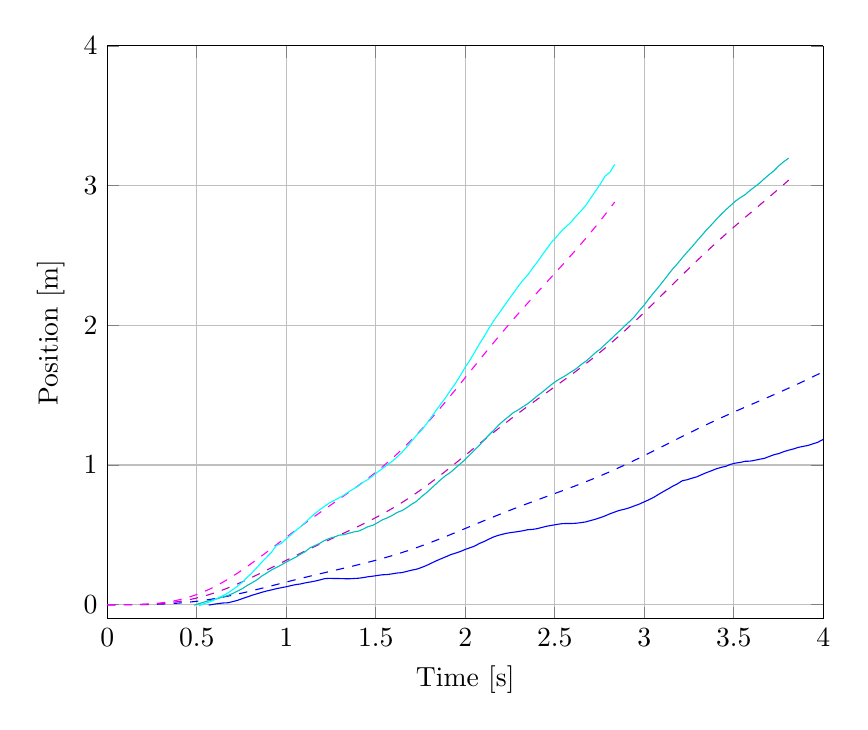
\begin{tikzpicture}

\begin{axis}[%
width=0.75\textwidth,
height=0.6\textwidth,
scale only axis,
separate axis lines,
every outer x axis line/.append style={black},
every x tick label/.append style={font=\color{black}},
xmin=0,
xmax=4,
xmajorgrids,
xlabel={Time [s]},
every outer y axis line/.append style={black},
every y tick label/.append style={font=\color{black}},
ymin=-0.1,
ymax=4,
ymajorgrids,
ylabel={Position [m]},
axis background/.style={fill=white},
legend style={at={(0.03,0.97)},anchor=north west,legend cell align=left,align=left,draw=black}
]
\addplot [color=blue,dashed]
  table[row sep=crcr]{%
0	0\\
0.027000027000027	1.21131502907475e-06\\
0.054000054000054	1.14801917282141e-05\\
0.081000081000081	4.46474255901955e-05\\
0.108000108000108	0.000119432137980353\\
0.135000135000135	0.000258960276800523\\
0.162000162000162	0.000490195837605392\\
0.189000189000189	0.000843287416294682\\
0.216000216000216	0.00135084458137138\\
0.243000243000243	0.0020471601093458\\
0.27000027000027	0.00296739532669735\\
0.297000297000297	0.0041467466192893\\
0.324000324000324	0.00561961158715232\\
0.351000351000351	0.00741877332987712\\
0.378000378000378	0.00957462094533417\\
0.405000405000405	0.0121144235210059\\
0.432000432000432	0.0150616737107003\\
0.459000459000459	0.0184355154461319\\
0.486000486000486	0.0222502684670326\\
0.513000513000513	0.0265150602064756\\
0.54000054000054	0.0312335731875582\\
0.567000567000567	0.0364039135262954\\
0.594000594000594	0.0420186034503083\\
0.621000621000621	0.0480646979931934\\
0.648000648000648	0.0545240232713019\\
0.675000675000675	0.0613735310540712\\
0.702000702000702	0.0685857617608187\\
0.729000729000729	0.076129405613168\\
0.756000756000756	0.0839699494963315\\
0.783000783000783	0.0920703951825632\\
0.81000081000081	0.100392032988319\\
0.837000837000837	0.108895253708102\\
0.864000864000864	0.117540380819835\\
0.891000891000891	0.126288504507704\\
0.918000918000918	0.135102299008676\\
0.945000945000945	0.143946805159212\\
0.972000972000972	0.152790160790777\\
0.999000999000999	0.161604262779603\\
1.02600102600103	0.170365346071941\\
1.05300105300105	0.179054466847287\\
1.08000108000108	0.187657879107868\\
1.10700110700111	0.196167296345915\\
1.13400113400113	0.204580032488503\\
1.16100116100116	0.212899018996526\\
1.18800118800119	0.221132697740341\\
1.21500121500122	0.229294792028864\\
1.24200124200124	0.237403960870342\\
1.26900126900127	0.24548334413185\\
1.2960012960013	0.253560008683279\\
1.32300132300132	0.261664307806597\\
1.35000135000135	0.269829168073885\\
1.37700137700138	0.278089319505352\\
1.4040014040014	0.286480486075627\\
1.43100143100143	0.295038554515304\\
1.45800145800146	0.303798739835378\\
1.48500148500149	0.312794766074367\\
1.51200151200151	0.322058080429839\\
1.53900153900154	0.331617118195354\\
1.56600156600157	0.341496634796889\\
1.59300159300159	0.351717119734644\\
1.62000162000162	0.362294305419716\\
1.64700164700165	0.373238781790788\\
1.67400167400167	0.384555725250376\\
1.7010017010017	0.396244747925247\\
1.72800172800173	0.408299870587744\\
1.75500175500176	0.42070961983284\\
1.78200178200178	0.433457247350858\\
1.80900180900181	0.446521066428758\\
1.83600183600184	0.459874898213966\\
1.86300186300186	0.473488617841301\\
1.89000189000189	0.487328788309764\\
1.91700191700192	0.501359368050765\\
1.94400194400194	0.515542476495958\\
1.97100197100197	0.529839200667349\\
1.998001998002	0.544210424903382\\
2.02500202500203	0.558617665322247\\
2.05200205200205	0.573023890519205\\
2.07900207900208	0.587394310300492\\
2.10600210600211	0.601697114965593\\
2.13300213300213	0.615904148746628\\
2.16000216000216	0.629991502473923\\
2.18700218700219	0.643940012328192\\
2.21400221400221	0.657735653622336\\
2.24100224100224	0.671369820883583\\
2.26800226800227	0.68483948802784\\
2.2950022950023	0.698147245076879\\
2.32200232200232	0.711301210606329\\
2.34900234900235	0.7243148218677\\
2.37600237600238	0.737206507239806\\
2.4030024030024	0.749999248273721\\
2.43000243000243	0.76272004104313\\
2.45700245700246	0.775399268744149\\
2.48400248400248	0.788069999456134\\
2.51100251100251	0.800767224633859\\
2.53800253800254	0.813527055215065\\
2.56500256500257	0.826385893166633\\
2.59200259200259	0.839379596836669\\
2.61900261900262	0.852542658616583\\
2.64600264600265	0.865907413143761\\
2.67300267300267	0.879503293597782\\
2.7000027000027	0.893356152576285\\
2.72700272700273	0.907487662604297\\
2.75400275400275	0.921914809564781\\
2.78100278100278	0.936649490277582\\
2.80800280800281	0.951698223144468\\
2.83500283500284	0.967061978270899\\
2.86200286200286	0.982736130825925\\
2.88900288900289	0.998710538669197\\
2.91600291600292	1.01496974251882\\
2.94300294300294	1.0314932842169\\
2.97000297000297	1.04825613603145\\
2.997002997003	1.06522923147157\\
3.02400302400302	1.08238008584248\\
3.05100305100305	1.09967349277774\\
3.07800307800308	1.11707228130161\\
3.10500310500311	1.13453811663336\\
3.13200313200313	1.1520323269755\\
3.15900315900316	1.16951673795286\\
3.18600318600319	1.18695449619991\\
3.21300321300321	1.20431086383521\\
3.24000324000324	1.22155396620768\\
3.26700326700327	1.23865547633619\\
3.29400329400329	1.25559122086772\\
3.32100332100332	1.27234169412024\\
3.34800334800335	1.2888924688146\\
3.37500337500338	1.30523449439046\\
3.4020034020034	1.32136427629441\\
3.42900342900343	1.33728393226725\\
3.45600345600346	1.35300112438493\\
3.48300348300348	1.36852886836223\\
3.51000351000351	1.38388522434977\\
3.53700353700354	1.39909287608187\\
3.56400356400356	1.41417860770848\\
3.59100359100359	1.42917268991234\\
3.61800361800362	1.44410818892353\\
3.64500364500365	1.45902021375271\\
3.67200367200367	1.47394511833366\\
3.6990036990037	1.48891967626504\\
3.72600372600373	1.50398024644802\\
3.75300375300375	1.5191619481182\\
3.78000378000378	1.53449786356095\\
3.80700380700381	1.55001828618527\\
3.83400383400383	1.56575003062501\\
3.86100386100386	1.58171582016046\\
3.88800388800389	1.59793376503872\\
3.91500391500392	1.61441694325532\\
3.94200394200394	1.63117309308774\\
3.96900396900397	1.64820442419316\\
3.996003996004	1.66550755145413\\
4.02300402300402	1.68307355303415\\
};
%\addlegendentry{1A model};

\addplot [color=blue,solid]
  table[row sep=crcr]{%
0.567000567000567	-0.00261892126032719\\
0.594000594000594	0.00288107873967281\\
0.621000621000621	0.00800158439638922\\
0.648000648000648	0.0124208419350871\\
0.675000675000675	0.0138618530265744\\
0.702000702000702	0.0222254690557172\\
0.729000729000729	0.0316716558252182\\
0.756000756000756	0.0440223802234323\\
0.783000783000783	0.055455444767822\\
0.81000081000081	0.0679897772093438\\
0.837000837000837	0.0781619055611524\\
0.864000864000864	0.0887124052207447\\
0.891000891000891	0.0981803723714605\\
0.918000918000918	0.106024896988125\\
0.945000945000945	0.114752771221417\\
0.972000972000972	0.121334624789779\\
0.999000999000999	0.128277014815113\\
1.02600102600103	0.136139024672902\\
1.05300105300105	0.14380227911307\\
1.08000108000108	0.148400953554954\\
1.10700110700111	0.156443052729083\\
1.13400113400113	0.162303559192205\\
1.16100116100116	0.169083809597856\\
1.18800118800119	0.177125743188929\\
1.21500121500122	0.18644776409286\\
1.24200124200124	0.188722017584237\\
1.26900126900127	0.187388920097679\\
1.2960012960013	0.187153510383954\\
1.32300132300132	0.186195452906042\\
1.35000135000135	0.185580486808929\\
1.37700137700138	0.187491251615686\\
1.4040014040014	0.189420839243924\\
1.43100143100143	0.194055880448798\\
1.45800145800146	0.200313710801204\\
1.48500148500149	0.204408803917773\\
1.51200151200151	0.209766051373772\\
1.53900153900154	0.214222874298238\\
1.56600156600157	0.215799148141135\\
1.59300159300159	0.221158601453681\\
1.62000162000162	0.22689869486653\\
1.64700164700165	0.229720169047663\\
1.67400167400167	0.238340278688733\\
1.7010017010017	0.247320169047663\\
1.72800172800173	0.253940882548948\\
1.75500175500176	0.265979136276488\\
1.78200178200178	0.279638624986541\\
1.80900180900181	0.29618242133571\\
1.83600183600184	0.312712412551968\\
1.86300186300186	0.327642069221545\\
1.89000189000189	0.342032287337583\\
1.91700191700192	0.357396512749419\\
1.94400194400194	0.368541218215834\\
1.97100197100197	0.379668272846432\\
1.998001998002	0.394601147395013\\
2.02500202500203	0.406828314107083\\
2.05200205200205	0.419235704587902\\
2.07900207900208	0.437990547010754\\
2.10600210600211	0.452523306897987\\
2.13300213300213	0.469792898129938\\
2.16000216000216	0.485616681239142\\
2.18700218700219	0.497116938739112\\
2.21400221400221	0.506116932489991\\
2.24100224100224	0.513476756475659\\
2.26800226800227	0.518495370134588\\
2.2950022950023	0.523171449325435\\
2.32200232200232	0.529268607275284\\
2.34900234900235	0.536645508391526\\
2.37600237600238	0.538900953554954\\
2.4030024030024	0.544474012562746\\
2.43000243000243	0.553652771221417\\
2.45700245700246	0.561947929506574\\
2.48400248400248	0.568042828437938\\
2.51100251100251	0.574335704587902\\
2.53800253800254	0.579581526547451\\
2.56500256500257	0.581544909710022\\
2.59200259200259	0.581164916580061\\
2.61900261900262	0.582970432855\\
2.64600264600265	0.587303030303313\\
2.67300267300267	0.592339736079729\\
2.7000027000027	0.602278925035064\\
2.72700272700273	0.611458750354408\\
2.75400275400275	0.622818831586097\\
2.78100278100278	0.635259277576381\\
2.80800280800281	0.650420841935087\\
2.83500283500284	0.663222132043342\\
2.86200286200286	0.675122874298238\\
2.88900288900289	0.683240727587286\\
2.91600291600292	0.693160099137209\\
2.94300294300294	0.706340727587286\\
2.97000297000297	0.718601584396389\\
2.997002997003	0.734665092277584\\
3.02400302400302	0.749629722628238\\
3.05100305100305	0.76677700605323\\
3.07800307800308	0.788073331686902\\
3.10500310500311	0.808452420547262\\
3.13200313200313	0.82758718940672\\
3.15900315900316	0.847857154244161\\
3.18600318600319	0.865529899939661\\
3.21300321300321	0.887277014815113\\
3.24000324000324	0.894417885792693\\
3.26700326700327	0.905598172943002\\
3.29400329400329	0.915336129839126\\
3.32100332100332	0.931041754250127\\
3.34800334800335	0.945286206729378\\
3.37500337500338	0.958467547916547\\
3.4020034020034	0.972369611786103\\
3.42900342900343	0.982648812620792\\
3.45600345600346	0.99074666210482\\
3.48300348300348	1.00481018744397\\
3.51000351000351	1.01348620672938\\
3.53700353700354	1.01855583180117\\
3.56400356400356	1.02634625565286\\
3.59100359100359	1.02746190556115\\
3.61800361800362	1.03380752269411\\
3.64500364500365	1.04103758785843\\
3.67200367200367	1.04774523945904\\
3.6990036990037	1.06130588895383\\
3.72600372600373	1.07376654333851\\
3.75300375300375	1.08209815766004\\
3.78000378000378	1.09565874293665\\
3.80700380700381	1.10599266853503\\
3.83400383400383	1.11488585499948\\
3.86100386100386	1.12592367904147\\
3.88800388800389	1.13335965243115\\
3.91500391500392	1.13971873017924\\
3.94200394200394	1.15149958795436\\
3.96900396900397	1.16202220761114\\
3.996003996004	1.18061895803307\\
4.02300402300402	1.19887858107219\\
};
%\addlegendentry{1A reality};

\addplot [color=mycolor1,dashed]
  table[row sep=crcr]{%
0	0\\
0.027000027000027	2.3746571857109e-06\\
0.054000054000054	2.2505722397885e-05\\
0.081000081000081	8.75266363055318e-05\\
0.108000108000108	0.000234134290298117\\
0.135000135000135	0.00050766470105449\\
0.162000162000162	0.000960977978671956\\
0.189000189000189	0.00165317731115195\\
0.216000216000216	0.00264819036744093\\
0.243000243000243	0.00401324457079671\\
0.27000027000027	0.00581727004639678\\
0.297000297000297	0.00812926564969586\\
0.324000324000324	0.0110166642995659\\
0.351000351000351	0.0145437338546106\\
0.378000378000378	0.0187700489819422\\
0.405000405000405	0.023749067892665\\
0.432000432000432	0.029526845492264\\
0.459000459000459	0.0361409114686546\\
0.486000486000486	0.0436193381828955\\
0.513000513000513	0.0519800190186354\\
0.54000054000054	0.0612301731795696\\
0.567000567000567	0.0713660879030346\\
0.594000594000594	0.0823731037936736\\
0.621000621000621	0.0942258435906169\\
0.648000648000648	0.106888679284334\\
0.675000675000675	0.120316427214912\\
0.702000702000702	0.13445525572913\\
0.729000729000729	0.149243785261458\\
0.756000756000756	0.164614356438353\\
0.783000783000783	0.180494438080668\\
0.81000081000081	0.196808143878091\\
0.837000837000837	0.213477824101032\\
0.864000864000864	0.230425697052746\\
0.891000891000891	0.247575484084409\\
0.918000918000918	0.264854011917999\\
0.945000945000945	0.282192746747762\\
0.972000972000972	0.299529226104691\\
0.999000999000999	0.316808356736251\\
1.02600102600103	0.333983549725192\\
1.05300105300105	0.35101766768082\\
1.08000108000108	0.367883763003543\\
1.10700110700111	0.384565590856349\\
1.13400113400113	0.401057885472512\\
1.16100116100116	0.417366393676357\\
1.18800118800119	0.433507664877104\\
1.21500121500122	0.449508602195199\\
1.24200124200124	0.465405784676512\\
1.26900126900127	0.481244575624816\\
1.2960012960013	0.497078036824647\\
1.32300132300132	0.512965672729764\\
1.35000135000135	0.528972032461675\\
1.37700137700138	0.545165200614452\\
1.4040014040014	0.561615210326478\\
1.43100143100143	0.57839241380228\\
1.45800145800146	0.595565846409948\\
1.48500148500149	0.613201620621036\\
1.51200151200151	0.63136138539711\\
1.53900153900154	0.65010088517505\\
1.56600156600157	0.669468650393901\\
1.59300159300159	0.689504848588708\\
1.62000162000162	0.710240321515878\\
1.64700164700165	0.731695829649268\\
1.67400167400167	0.753881520787865\\
1.7010017010017	0.776796634546524\\
1.72800172800173	0.800429449271022\\
1.75500175500176	0.824757472543588\\
1.78200178200178	0.849747871044256\\
1.80900180900181	0.875358130226674\\
1.83600183600184	0.901536929171934\\
1.86300186300186	0.928225211213641\\
1.89000189000189	0.955357426587457\\
1.91700191700192	0.982862919545064\\
1.94400194400194	1.01066742917029\\
1.97100197100197	1.0386946706152\\
1.998001998002	1.06686796169178\\
2.02500202500203	1.09511185875054\\
2.05200205200205	1.1233537655723\\
2.07900207900208	1.15152547959898\\
2.10600210600211	1.17956464121968\\
2.13300213300213	1.20741605397854\\
2.16000216000216	1.23503284643403\\
2.18700218700219	1.26237744991071\\
2.21400221400221	1.28942237046755\\
2.24100224100224	1.3161507379698\\
2.26800226800227	1.34255662009418\\
2.2950022950023	1.36864509430913\\
2.32200232200232	1.39443207623815\\
2.34900234900235	1.41994390821589\\
2.37600237600238	1.44521671716318\\
2.4030024030024	1.47029555602175\\
2.43000243000243	1.49523334778752\\
2.45700245700246	1.52008965555784\\
2.48400248400248	1.5449293058645\\
2.51100251100251	1.56982089581687\\
2.53800253800254	1.59483521715429\\
2.56500256500257	1.62004363214845\\
2.59200259200259	1.64551643736297\\
2.61900261900262	1.67132125154538\\
2.64600264600265	1.69752146339074\\
2.67300267300267	1.72417477358773\\
2.7000027000027	1.75133186346638\\
2.72700272700273	1.77903521975892\\
2.75400275400275	1.80731814152304\\
2.78100278100278	1.83620395123724\\
2.80800280800281	1.86570542755054\\
2.83500283500284	1.89582447225384\\
2.86200286200286	1.92655201884686\\
2.88900288900289	1.95786818471783\\
2.91600291600292	1.98974266355174\\
2.94300294300294	2.02213534925689\\
2.97000297000297	2.05499717756661\\
2.997002997003	2.08827116664723\\
3.02400302400302	2.1218936336318\\
3.05100305100305	2.15579556009893\\
3.07800307800308	2.18990407621504\\
3.10500310500311	2.22414403062777\\
3.13200313200313	2.2584396112985\\
3.15900315900316	2.29271598133333\\
3.18600318600319	2.32690089354042\\
3.21300321300321	2.36092624791456\\
3.24000324000324	2.39472955751605\\
3.26700326700327	2.42825529024323\\
3.29400329400329	2.46145605675058\\
3.32100332100332	2.49429361817631\\
3.34800334800335	2.5267396913395\\
3.37500337500338	2.55877653355753\\
3.4020034020034	2.59039729412171\\
3.42900342900343	2.62160612464273\\
3.45600345600346	2.65241804582391\\
3.48300348300348	2.68285857362101\\
3.51000351000351	2.71296311308173\\
3.53700353700354	2.742776133309\\
3.56400356400356	2.77235014184434\\
3.59100359100359	2.80174448121429\\
3.61800361800362	2.83102397432534\\
3.64500364500365	2.86025744874293\\
3.67200367200367	2.8895161725749\\
3.6990036990037	2.9188722366384\\
3.72600372600373	2.94839691877929\\
3.75300375300375	2.97815906660796\\
3.78000378000378	3.00822353450562\\
3.80700380700381	3.03864970955131\\
};
%\addlegendentry{2A model};

\addplot [color=mycolor2,solid]
  table[row sep=crcr]{%
0.486000486000486	-0.00285311943372782\\
0.513000513000513	0.00756033112982135\\
0.54000054000054	0.0181297764780982\\
0.567000567000567	0.0284122868061577\\
0.594000594000594	0.0352396309796456\\
0.621000621000621	0.0447810367561761\\
0.648000648000648	0.0564742252636437\\
0.675000675000675	0.0661948821015082\\
0.702000702000702	0.0804238665879121\\
0.729000729000729	0.0982459580886276\\
0.756000756000756	0.115578388282846\\
0.783000783000783	0.138468856578046\\
0.81000081000081	0.157769571656618\\
0.837000837000837	0.178355092277584\\
0.864000864000864	0.205615563588257\\
0.891000891000891	0.226029394526908\\
0.918000918000918	0.249005073423014\\
0.945000945000945	0.265812663116783\\
0.972000972000972	0.284459435308496\\
0.999000999000999	0.304188233952523\\
1.02600102600103	0.322293521880269\\
1.05300105300105	0.339496928541303\\
1.08000108000108	0.361604928743789\\
1.10700110700111	0.380268458482396\\
1.13400113400113	0.408216886695966\\
1.16100116100116	0.423076206729378\\
1.18800118800119	0.439955271594511\\
1.21500121500122	0.460258607275284\\
1.24200124200124	0.474794792057164\\
1.26900126900127	0.484624624789779\\
1.2960012960013	0.497554211434034\\
1.32300132300132	0.501265832472592\\
1.35000135000135	0.511506155945099\\
1.37700137700138	0.520576215541883\\
1.4040014040014	0.526856051373772\\
1.43100143100143	0.541251201168716\\
1.45800145800146	0.558889911943576\\
1.48500148500149	0.568990063084593\\
1.51200151200151	0.588112207611138\\
1.53900153900154	0.608673649362602\\
1.56600156600157	0.621666341093183\\
1.59300159300159	0.639380034950618\\
1.62000162000162	0.660326756706448\\
1.64700164700165	0.673721350404908\\
1.67400167400167	0.694518681599306\\
1.7010017010017	0.719076755019187\\
1.72800172800173	0.739849717674317\\
1.75500175500176	0.772363073669581\\
1.78200178200178	0.799405386287256\\
1.80900180900181	0.831115956878079\\
1.83600183600184	0.862837839296278\\
1.86300186300186	0.894949862137039\\
1.89000189000189	0.92326852692051\\
1.91700191700192	0.94632878943616\\
1.94400194400194	0.976471717406223\\
1.97100197100197	1.00699665393981\\
1.998001998002	1.036460432855\\
2.02500202500203	1.07239753384104\\
2.05200205200205	1.10673305718896\\
2.07900207900208	1.14036583247259\\
2.10600210600211	1.17959001800514\\
2.13300213300213	1.21484431939147\\
2.16000216000216	1.24903305272908\\
2.18700218700219	1.28630195437833\\
2.21400221400221	1.31708289812994\\
2.24100224100224	1.34480110059006\\
2.26800226800227	1.37394162009696\\
2.2950022950023	1.39315148912462\\
2.32200232200232	1.41616245744891\\
2.34900234900235	1.43873957454316\\
2.37600237600238	1.46555421143403\\
2.4030024030024	1.49509178122643\\
2.43000243000243	1.52080606803656\\
2.45700245700246	1.54982018064703\\
2.48400248400248	1.57755379806243\\
2.51100251100251	1.60296015406451\\
2.53800253800254	1.62293853472087\\
2.56500256500257	1.64349880391777\\
2.59200259200259	1.66642934671602\\
2.61900261900262	1.68807050906029\\
2.64600264600265	1.71713534689349\\
2.67300267300267	1.74146634109318\\
2.7000027000027	1.77157042672338\\
2.72700272700273	1.80311130033251\\
2.75400275400275	1.82919795619425\\
2.78100278100278	1.86217498673361\\
2.80800280800281	1.89371595687808\\
2.83500283500284	1.92725450899139\\
2.86200286200286	1.95917744895224\\
2.88900288900289	1.99255950776563\\
2.91600291600292	2.02448274645649\\
2.94300294300294	2.05784164668268\\
2.97000297000297	2.10116634109318\\
2.997002997003	2.1400960508576\\
3.02400302400302	2.18592876889282\\
3.05100305100305	2.23027242133571\\
3.07800307800308	2.27010116083157\\
3.10500310500311	2.31426159587457\\
3.13200313200313	2.35898545290604\\
3.15900315900316	2.40280787479502\\
3.18600318600319	2.44139859107647\\
3.21300321300321	2.48379227911307\\
3.24000324000324	2.52423776409286\\
3.26700326700327	2.56158127615184\\
3.29400329400329	2.60308581719778\\
3.32100332100332	2.64262681932992\\
3.34800334800335	2.68252674244889\\
3.37500337500338	2.71844656739572\\
3.4020034020034	2.75670519581286\\
3.42900342900343	2.79314343071479\\
3.45600345600346	2.82668293157475\\
3.48300348300348	2.85790519581286\\
3.51000351000351	2.88878683798474\\
3.53700353700354	2.91334388398769\\
3.56400356400356	2.9353698615297\\
3.59100359100359	2.96499859107647\\
3.61800361800362	2.9915594353085\\
3.64500364500365	3.01811902438855\\
3.67200367200367	3.05028830837225\\
3.6990036990037	3.07937459496522\\
3.72600372600373	3.10684067356016\\
3.75300375300375	3.14258140737006\\
3.78000378000378	3.17129384733611\\
3.80700380700381	3.19586852692051\\
};
%\addlegendentry{2A reality};

\addplot [color=mycolor3,dashed]
  table[row sep=crcr]{%
0	0\\
0.027000027000027	3.60995865100495e-06\\
0.054000054000054	3.42132446553707e-05\\
0.081000081000081	0.000133058169333157\\
0.108000108000108	0.000355931421109764\\
0.135000135000135	0.000771752904128291\\
0.162000162000162	0.00146088066454676\\
0.189000189000189	0.00251316348816534\\
0.216000216000216	0.00402578434646323\\
0.243000243000243	0.00610094250408995\\
0.27000027000027	0.00884342567659309\\
0.297000297000297	0.0123581260634265\\
0.324000324000324	0.0167475553240876\\
0.351000351000351	0.0221094135870596\\
0.378000378000378	0.0285342663816395\\
0.405000405000405	0.0361033809883443\\
0.432000432000432	0.0448867701675327\\
0.459000459000459	0.054941486626591\\
0.486000486000486	0.0663102060255129\\
0.513000513000513	0.0790201299222689\\
0.54000054000054	0.0930822329649013\\
0.567000567000567	0.108490871004108\\
0.594000594000594	0.125223758797453\\
0.621000621000621	0.143242317781695\\
0.648000648000648	0.162492386184771\\
0.675000675000675	0.182905275715598\\
0.702000702000702	0.204399151386202\\
0.729000729000729	0.226880703857065\\
0.756000756000756	0.250247077211839\\
0.783000783000783	0.274388009405461\\
0.81000081000081	0.299188137915684\\
0.837000837000837	0.32452941946672\\
0.864000864000864	0.350293610166043\\
0.891000891000891	0.376364751057612\\
0.918000918000918	0.402631603976353\\
0.945000945000945	0.428989983692306\\
0.972000972000972	0.455344934633899\\
0.999000999000999	0.481612703927331\\
1.02600102600103	0.507722467006479\\
1.05300105300105	0.533617767534984\\
1.08000108000108	0.559257639717507\\
1.10700110700111	0.584617388120005\\
1.13400113400113	0.609689007713263\\
1.16100116100116	0.63448123483123\\
1.18800118800119	0.659019227919234\\
1.21500121500122	0.683343885155328\\
1.24200124200124	0.70751081407894\\
1.26900126900127	0.731588976076109\\
1.2960012960013	0.755659035778882\\
1.32300132300132	0.779811451978075\\
1.35000135000135	0.804144352378607\\
1.37700137700138	0.82876123931793\\
1.4040014040014	0.853768577314494\\
1.43100143100143	0.879273315931749\\
1.45800145800146	0.90538040287573\\
1.48500148500149	0.932190342459251\\
1.51200151200151	0.959796853558233\\
1.53900153900154	0.988284678978233\\
1.56600156600157	1.01772759479073\\
1.59300159300159	1.04818666376364\\
1.62000162000162	1.07970877159737\\
1.64700164700165	1.11232547840621\\
1.67400167400167	1.14605221089468\\
1.7010017010017	1.18088781312376\\
1.72800172800173	1.216814465811\\
1.75500175500176	1.25379797593747\\
1.78200178200178	1.29178843022384\\
1.80900180900181	1.33072119797085\\
1.83600183600184	1.3705182610139\\
1.86300186300186	1.41108984128942\\
1.89000189000189	1.45233628991326\\
1.91700191700192	1.49415019587406\\
1.94400194400194	1.53641866757706\\
1.97100197100197	1.5790257366423\\
1.998001998002	1.62185483065265\\
2.02500202500203	1.66479126001977\\
2.05200205200205	1.70772466382456\\
2.07900207900208	1.75055136040048\\
2.10600210600211	1.79317655054103\\
2.13300213300213	1.83551632448253\\
2.16000216000216	1.87749942816486\\
2.18700218700219	1.91906874961174\\
2.21400221400221	1.96018249247845\\
2.24100224100224	2.00081501075207\\
2.26800226800227	2.04095728610277\\
2.2950022950023	2.08061703730832\\
2.32200232200232	2.11981845933173\\
2.34900234900235	2.15860159784334\\
2.37600237600238	2.1970213730612\\
2.4030024030024	2.23514627455832\\
2.43000243000243	2.27305675598002\\
2.45700245700246	2.31084336526722\\
2.48400248400248	2.34860465184452\\
2.51100251100251	2.38644489717616\\
2.53800253800254	2.42447171900727\\
2.56500256500257	2.46279360240749\\
2.59200259200259	2.50151741235483\\
2.61900261900262	2.54074594300586\\
2.64600264600265	2.58057555798289\\
2.67300267300267	2.62109397398943\\
2.7000027000027	2.66237823688576\\
2.72700272700273	2.70449293508805\\
2.75400275400275	2.74748868989108\\
2.78100278100278	2.79140095617378\\
2.80800280800281	2.83624916006421\\
2.83500283500284	2.88203619266872\\
};
%\addlegendentry{3A model};

\addplot [color=mycolor4,solid]
  table[row sep=crcr]{%
0.513000513000513	-0.00766666962215803\\
0.54000054000054	0.00755576607290901\\
0.567000567000567	0.0166742480728837\\
0.594000594000594	0.0322875949681057\\
0.621000621000621	0.0491422287083981\\
0.648000648000648	0.0647557133848187\\
0.675000675000675	0.0841289733259071\\
0.702000702000702	0.108830979890807\\
0.729000729000729	0.133756495933387\\
0.756000756000756	0.161753556581554\\
0.783000783000783	0.197277655290258\\
0.81000081000081	0.228747563248111\\
0.837000837000837	0.26672679216136\\
0.864000864000864	0.304539571656618\\
0.891000891000891	0.340686450857816\\
0.918000918000918	0.375503637844332\\
0.945000945000945	0.423579757958617\\
0.972000972000972	0.437900388729493\\
0.999000999000999	0.470018949962215\\
1.02600102600103	0.49980957454316\\
1.05300105300105	0.529977885792693\\
1.08000108000108	0.55790776409286\\
1.10700110700111	0.587551276151842\\
1.13400113400113	0.622256192418405\\
1.16100116100116	0.652296639012197\\
1.18800118800119	0.680356494062998\\
1.21500121500122	0.705013883987688\\
1.24200124200124	0.729327547916547\\
1.26900126900127	0.746966928541303\\
1.2960012960013	0.764618110847937\\
1.32300132300132	0.78481194111983\\
1.35000135000135	0.808652668535034\\
1.37700137700138	0.829560958990506\\
1.4040014040014	0.851538662940836\\
1.43100143100143	0.876983079112444\\
1.45800145800146	0.897136341093183\\
1.48500148500149	0.923337948960022\\
1.51200151200151	0.950087144356317\\
1.53900153900154	0.975978270460101\\
1.56600156600157	1.00245150293499\\
1.59300159300159	1.02737674173139\\
1.62000162000162	1.0579871157077\\
1.64700164700165	1.09119689913572\\
1.67400167400167	1.12920117184002\\
1.7010017010017	1.17117843798558\\
1.72800172800173	1.21194823738393\\
1.75500175500176	1.24917079775361\\
1.78200178200178	1.29076419316255\\
1.80900180900181	1.33837138187383\\
1.83600183600184	1.38834397313154\\
1.86300186300186	1.43514507688342\\
1.89000189000189	1.48085151151145\\
1.91700191700192	1.53252469019568\\
1.94400194400194	1.58134102107647\\
1.97100197100197	1.63669557967574\\
1.998001998002	1.69563913627649\\
2.02500202500203	1.74806095899051\\
2.05200205200205	1.80519757866187\\
2.07900207900208	1.86609659180069\\
2.10600210600211	1.91999930678663\\
2.13300213300213	1.97914503281176\\
2.16000216000216	2.03417414225305\\
2.18700218700219	2.08145485296241\\
2.21400221400221	2.1314561924184\\
2.24100224100224	2.18057643970336\\
2.26800226800227	2.22755537013459\\
2.2950022950023	2.2766561924184\\
2.32200232200232	2.32141555747003\\
2.34900234900235	2.36003055971434\\
2.37600237600238	2.40751074235743\\
2.4030024030024	2.45336921667455\\
2.43000243000243	2.50254620672938\\
2.45700245700246	2.55042405810106\\
2.48400248400248	2.59599462478978\\
2.51100251100251	2.63525092415267\\
2.53800253800254	2.67414416718697\\
2.56500256500257	2.7068737108012\\
2.59200259200259	2.73885914814114\\
2.61900261900262	2.78010027868873\\
2.64600264600265	2.81793832547509\\
2.67300267300267	2.85741318663039\\
2.7000027000027	2.90821688056627\\
2.72700272700273	2.95850797395115\\
2.75400275400275	3.00936297474819\\
2.78100278100278	3.06646228768108\\
2.80800280800281	3.09500965404878\\
2.83500283500284	3.1508438397686\\
};
%\addlegendentry{3A reality};

\end{axis}

\begin{axis}[%
width=0.85\textwidth,
height=0.6\textwidth,
at={(1.85in,0.746in)},
scale only axis,
every outer x axis line/.append style={black},
every x tick label/.append style={font=\color{black}},
xmin=0,
xmax=1,
every outer y axis line/.append style={black},
every y tick label/.append style={font=\color{black}},
ymin=0,
ymax=1,
hide axis,
axis x line*=bottom,
axis y line*=left
]
\end{axis}
\end{tikzpicture}%
              \end{figure}}	     	
    \end{itemize}           
  \end{minipage}
\end{frame} 
%%%%%%%%%%%%%%%%
% Hoist model
%%%%%%%%%%%%%%%%

\subsection{Hejsningsmodel}
\begin{frame}{Model opstilling}{Hejsningsmodel}
  \begin{minipage}[t]{0.45\linewidth}
    \begin{itemize}
    	\item<1->[] Fritlegeme diagram for y-aksen 
      	\item<1->[] {
              \begin{figure}[H]
              \centering
              \scalebox{0.75}{\input{Billeder/Daniel/FBDhoist.ralf}}
              \end{figure}}    
    \end{itemize}           
  \end{minipage}
  \begin{minipage}[t]{0.48\linewidth}
\begin{itemize}
    	\item<2->[] Resulterende kraft  
    	\item<2->[] {
    		\begin{equation*}
				m_y \ddot{y} = F_g - F_a - F_B = F_g - F_a - B_y \dot{y}
			\end{equation*}}
	\end{itemize}
	\bigskip
	\begin{itemize}
	    	\item<3->[] Overføringsfunktion
    		\item<3->[] {
    		\begin{equation*}
				\frac{Y(s)}{F_a(s)} = \frac{1}{m_y s^2 + B_y s}
			\end{equation*}}
	\end{itemize}                
  \end{minipage}
\end{frame} 
%%%%%%%%%%%%%%%%

\begin{frame}{Model opstilling}{Hejsningsmodel}
  \begin{minipage}[t]{0.48\linewidth}
    \begin{itemize}
      	\item<1->[] {
              \begin{figure}[H]
              \centering
              % This file was created by matlab2tikz.
%
%The latest updates can be retrieved from
%  http://www.mathworks.com/matlabcentral/fileexchange/22022-matlab2tikz-matlab2tikz
%where you can also make suggestions and rate matlab2tikz.
%
\definecolor{mycolor1}{rgb}{0.75000,0.00000,0.75000}%
\definecolor{mycolor2}{rgb}{0.00000,0.75000,0.75000}%
\definecolor{mycolor3}{rgb}{1.00000,0.00000,1.00000}%
\definecolor{mycolor4}{rgb}{0.00000,1.00000,1.00000}%
%
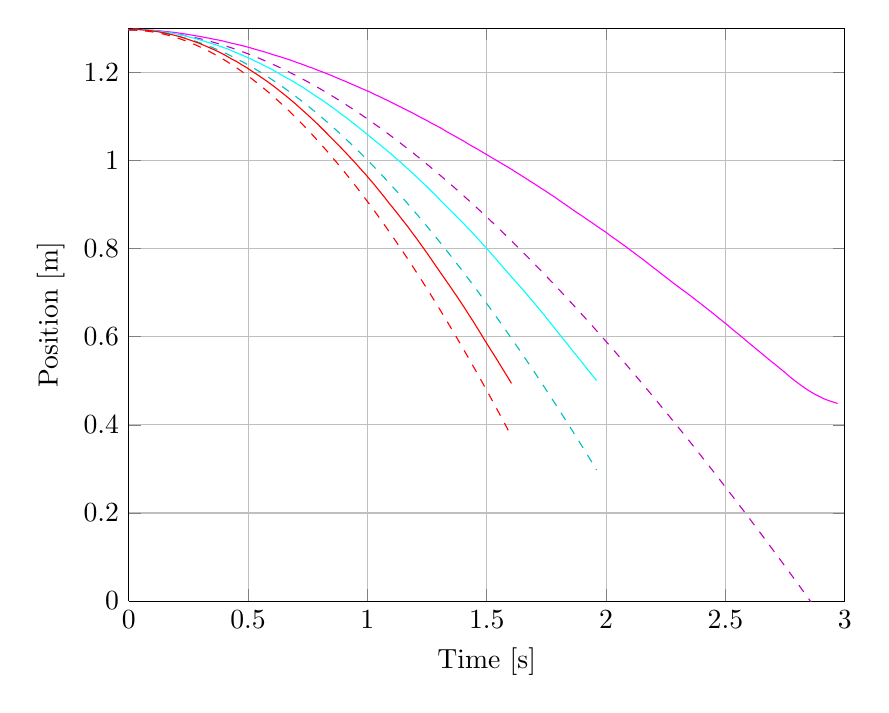
\begin{tikzpicture}

\begin{axis}[%
width=0.75\textwidth,
height=0.6\textwidth,
scale only axis,
separate axis lines,
every outer x axis line/.append style={black},
every x tick label/.append style={font=\color{black}},
xmin=0,
xmax=3,
xmajorgrids,
xlabel={Time [s] },
every outer y axis line/.append style={black},
every y tick label/.append style={font=\color{black}},
ymin=0,
ymax=1.3,
ymajorgrids,
ylabel={Position [m]},
axis background/.style={fill=white},
legend style={legend cell align=left,align=left,draw=black}
]
\addplot [color=mycolor1,dashed]
  table[row sep=crcr]{%
0	1.296\\
0.0198000198000198	1.2959088948787\\
0.0396000396000396	1.29563665088366\\
0.0594000594000594	1.29518486444088\\
0.0792000792000792	1.29455511790663\\
0.099000099000099	1.29374897969145\\
0.118800118800119	1.29276800438306\\
0.138600138600139	1.29161373286817\\
0.158400158400158	1.29028769245323\\
0.178200178200178	1.28879139698414\\
0.198000198000198	1.28712634696485\\
0.217800217800218	1.28529402967497\\
0.237600237600238	1.2832959192863\\
0.257400257400257	1.28113347697839\\
0.277200277200277	1.278808151053\\
0.297000297000297	1.27632137704761\\
0.316800316800317	1.27367457784793\\
0.336600336600337	1.27086916379938\\
0.356400356400356	1.26790653281764\\
0.376200376200376	1.26478807049817\\
0.396000396000396	1.2615151502248\\
0.415800415800416	1.25808913327736\\
0.435600435600436	1.25451136893836\\
0.455400455400455	1.25078319459869\\
0.475200475200475	1.24690593586248\\
0.495000495000495	1.24288090665094\\
0.514800514800515	1.23870940930533\\
0.534600534600535	1.23439273468904\\
0.554400554400554	1.22993216228872\\
0.574200574200574	1.22532896031456\\
0.594000594000594	1.22058438579965\\
0.613800613800614	1.21569968469855\\
0.633600633600634	1.21067609198484\\
0.653400653400653	1.20551483174797\\
0.673200673200673	1.20021711728915\\
0.693000693000693	1.19478415121644\\
0.712800712800713	1.18921712553898\\
0.732600732600733	1.18351722176043\\
0.752400752400752	1.1776856109715\\
0.772200772200772	1.17172345394181\\
0.792000792000792	1.16563190121076\\
0.811800811800812	1.15941209317776\\
0.831600831600832	1.15306516019156\\
0.851400851400851	1.14659222263885\\
0.871200871200871	1.13999439103203\\
0.891000891000891	1.13327276609626\\
0.910800910800911	1.12642843885573\\
0.930600930600931	1.11946249071911\\
0.95040095040095	1.11237599356434\\
0.97020097020097	1.1051700098226\\
0.99000099000099	1.09784559256158\\
1.00980100980101	1.090403785568\\
1.02960102960103	1.08284562342941\\
1.04940104940105	1.07517213161524\\
1.06920106920107	1.0673843265572\\
1.08900108900109	1.05948321572891\\
1.10880110880111	1.05146979772483\\
1.12860112860113	1.04334506233856\\
1.14840114840115	1.03510999064038\\
1.16820116820117	1.02676555505411\\
1.18800118800119	1.01831271943336\\
1.20780120780121	1.00975243913702\\
1.22760122760123	1.00108566110416\\
1.24740124740125	0.992313323928197\\
1.26720126720127	0.983436357930488\\
1.28700128700129	0.974455685233206\\
1.30680130680131	0.965372219831616\\
1.32660132660133	0.956186867665693\\
1.34640134640135	0.946900526691117\\
1.36620136620137	0.937514086949641\\
1.38600138600139	0.928028430638841\\
1.40580140580141	0.918444432181243\\
1.42560142560143	0.908762958292854\\
1.44540144540145	0.898984868051074\\
1.46520146520147	0.889111012962024\\
1.48500148500149	0.879142237027269\\
1.5048015048015	0.86907937680996\\
1.52460152460152	0.85892326150039\\
1.54440154440154	0.848674712980973\\
1.56420156420156	0.838334545890651\\
1.58400158400158	0.827903567688731\\
1.6038016038016	0.817382578718163\\
1.62360162360162	0.806772372268258\\
1.64340164340164	0.796073734636852\\
1.66320166320166	0.785287445191925\\
1.68300168300168	0.774414276432677\\
1.7028017028017	0.763454994050062\\
1.72260172260172	0.752410356986793\\
1.74240174240174	0.741281117496813\\
1.76220176220176	0.73006802120425\\
1.78200178200178	0.718771807161842\\
1.8018018018018	0.707393207908855\\
1.82160182160182	0.69593294952849\\
1.84140184140184	0.684391751704777\\
1.86120186120186	0.672770327778978\\
1.88100188100188	0.661069384805483\\
1.9008019008019	0.649289623607221\\
1.92060192060192	0.637431738830579\\
1.94040194040194	0.625496418999835\\
1.96020196020196	0.613484346571118\\
1.98000198000198	0.601396197985886\\
1.999801999802	0.589232643723933\\
2.01960201960202	0.576994348355935\\
2.03940203940204	0.564681970595525\\
2.05920205920206	0.552296163350915\\
2.07900207900208	0.539837573776059\\
2.0988020988021	0.527306843321369\\
2.11860211860212	0.51470460778398\\
2.13840213840214	0.502031497357573\\
2.15820215820216	0.489288136681764\\
2.17800217800218	0.476475144891049\\
2.1978021978022	0.463593135663323\\
2.21760221760222	0.450642717267974\\
2.23740223740224	0.437624492613543\\
2.25720225720226	0.42453905929498\\
2.27700227700228	0.411387009640462\\
2.2968022968023	0.398168930757824\\
2.31660231660232	0.384885404580555\\
2.33640233640234	0.371537007913409\\
2.35620235620236	0.358124312477603\\
2.37600237600238	0.34464788495562\\
2.3958023958024	0.331108287035616\\
2.41560241560242	0.317506075455437\\
2.43540243540244	0.303841802046249\\
2.45520245520246	0.290116013775777\\
2.47500247500248	0.276329252791175\\
2.49480249480249	0.262482056461505\\
2.51460251460251	0.248574957419849\\
2.53440253440253	0.234608483605051\\
2.55420255420255	0.220583158303086\\
2.57400257400257	0.206499500188068\\
2.59380259380259	0.192358023362895\\
2.61360261360261	0.178159237399537\\
2.63340263340263	0.163903647378969\\
2.65320265320265	0.149591753930749\\
2.67300267300267	0.135224053272251\\
2.69280269280269	0.120801037247551\\
2.71260271260271	0.106323193365972\\
2.73240273240273	0.0917910048402806\\
2.75220275220275	0.0772049506245625\\
2.77200277200277	0.0625655054517489\\
2.79180279180279	0.0478731398708219\\
2.81160281160281	0.0331283202836872\\
2.83140283140283	0.0183315089817244\\
2.85120285120285	0.00348316418201389\\
2.87100287100287	-0.0114162599367555\\
};
%\addlegendentry{2A model};

\addplot [color=mycolor2,dashed]
  table[row sep=crcr]{%
0	1.296\\
0.0198000198000198	1.29586675051176\\
0.0396000396000396	1.29546856902095\\
0.0594000594000594	1.29480779044516\\
0.0792000792000792	1.2938867291237\\
0.099000099000099	1.29270767899898\\
0.118800118800119	1.29127291379628\\
0.138600138600139	1.28958468720191\\
0.158400158400158	1.28764523303985\\
0.178200178200178	1.28545676544677\\
0.198000198000198	1.28302147904555\\
0.217800217800218	1.28034154911729\\
0.237600237600238	1.27741913177171\\
0.257400257400257	1.27425636411618\\
0.277200277200277	1.27085536442314\\
0.297000297000297	1.26721823229615\\
0.316800316800317	1.26334704883436\\
0.336600336600337	1.25924387679566\\
0.356400356400356	1.25491076075828\\
0.376200376200376	1.25034972728102\\
0.396000396000396	1.24556278506209\\
0.415800415800416	1.24055192509647\\
0.435600435600436	1.23531912083199\\
0.455400455400455	1.22986632832393\\
0.475200475200475	1.22419548638833\\
0.495000495000495	1.21830851675391\\
0.514800514800515	1.2122073242127\\
0.534600534600535	1.20589379676926\\
0.554400554400554	1.19936980578865\\
0.574200574200574	1.19263720614309\\
0.594000594000594	1.18569783635731\\
0.613800613800614	1.17855351875262\\
0.633600633600634	1.17120605958973\\
0.653400653400653	1.16365724921026\\
0.673200673200673	1.15590886217709\\
0.693000693000693	1.14796265741337\\
0.712800712800713	1.13982037834041\\
0.732600732600733	1.13148375301425\\
0.752400752400752	1.12295449426113\\
0.772200772200772	1.11423429981167\\
0.792000792000792	1.10532485243393\\
0.811800811800812	1.09622782006528\\
0.831600831600832	1.08694485594311\\
0.851400851400851	1.07747759873439\\
0.871200871200871	1.06782767266405\\
0.891000891000891	1.0579966876423\\
0.910800910800911	1.04798623939078\\
0.930600930600931	1.03779790956758\\
0.95040095040095	1.02743326589124\\
0.97020097020097	1.01689386226355\\
0.99000099000099	1.00618123889134\\
1.00980100980101	0.995296922407195\\
1.02960102960103	0.98424242598906\\
1.04940104940105	0.97301924947884\\
1.06920106920107	0.961628879499923\\
1.08900108900109	0.950072789573683\\
1.10880110880111	0.93835244023495\\
1.12860112860113	0.926469279146465\\
1.14840114840115	0.914424741212326\\
1.16820116820117	0.90222024869043\\
1.18800118800119	0.88985721130393\\
1.20780120780121	0.877337026351708\\
1.22760122760123	0.86466107881787\\
1.24740124740125	0.851830741480282\\
1.26720126720127	0.838847375018149\\
1.28700128700129	0.825712328118638\\
1.30680130680131	0.812426937582572\\
1.32660132660133	0.798992528429186\\
1.34640134640135	0.785410413999959\\
1.36620136620137	0.771681896061538\\
1.38600138600139	0.757808264907746\\
1.40580140580141	0.743790799460699\\
1.42560142560143	0.729630767371022\\
1.44540144540145	0.715329425117194\\
1.46520146520147	0.700888018104008\\
1.48500148500149	0.686307780760166\\
1.5048015048015	0.671589936635016\\
1.52460152460152	0.656735698494434\\
1.54440154440154	0.641746268415861\\
1.56420156420156	0.626622837882502\\
1.58400158400158	0.611366587876701\\
1.6038016038016	0.595978688972482\\
1.62360162360162	0.580460301427283\\
1.64340164340164	0.564812575272879\\
1.66320166320166	0.549036650405502\\
1.68300168300168	0.533133656675171\\
1.7028017028017	0.517104713974229\\
1.72260172260172	0.500950932325107\\
1.74240174240174	0.484673411967303\\
1.76220176220176	0.468273243443609\\
1.78200178200178	0.451751507685567\\
1.8018018018018	0.435109276098176\\
1.82160182160182	0.418347610643852\\
1.84140184140184	0.401467563925649\\
1.86120186120186	0.384470179269744\\
1.88100188100188	0.367356490807199\\
1.9008019008019	0.350127523554996\\
1.92060192060192	0.332784293496367\\
1.94040194040194	0.315327807660408\\
1.96020196020196	0.297759064200992\\
};
%\addlegendentry{3A model};

\addplot [color=red,dashed]
  table[row sep=crcr]{%
0	1.296\\
0.0198000198000198	1.29582443072874\\
0.0396000396000396	1.29529978755681\\
0.0594000594000594	1.29442914696715\\
0.0792000792000792	1.29321555832881\\
0.099000099000099	1.29166204413595\\
0.118800118800119	1.28977160024464\\
0.138600138600139	1.28754719610768\\
0.158400158400158	1.28499177500725\\
0.178200178200178	1.28210825428563\\
0.198000198000198	1.27889952557372\\
0.217800217800218	1.27536845501773\\
0.237600237600238	1.27151788350374\\
0.257400257400257	1.26735062688031\\
0.277200277200277	1.2628694761792\\
0.297000297000297	1.258077197834\\
0.316800316800317	1.25297653389702\\
0.336600336600337	1.2475702022541\\
0.356400356400356	1.2418608968376\\
0.376200376200376	1.23585128783754\\
0.396000396000396	1.22954402191084\\
0.415800415800416	1.2229417223887\\
0.435600435600436	1.21604698948218\\
0.455400455400455	1.20886240048601\\
0.475200475200475	1.20139050998049\\
0.495000495000495	1.19363385003173\\
0.514800514800515	1.18559493039004\\
0.534600534600535	1.17727623868663\\
0.554400554400554	1.16868024062855\\
0.574200574200574	1.15980938019188\\
0.594000594000594	1.15066607981331\\
0.613800613800614	1.1412527405799\\
0.633600633600634	1.1315717424173\\
0.653400653400653	1.12162544427624\\
0.673200673200673	1.11141618431737\\
0.693000693000693	1.10094628009447\\
0.712800712800713	1.09021802873613\\
0.732600732600733	1.0792337071257\\
0.752400752400752	1.06799557207974\\
0.772200772200772	1.05650586052489\\
0.792000792000792	1.04476678967313\\
0.811800811800812	1.03278055719555\\
0.831600831600832	1.02054934139459\\
0.851400851400851	1.0080753013747\\
0.871200871200871	0.995360577211558\\
0.891000891000891	0.982407290119787\\
0.910800910800911	0.969217542619159\\
0.930600930600931	0.955793418699374\\
0.95040095040095	0.942136983983366\\
0.97020097020097	0.928250285889171\\
0.99000099000099	0.914135353790377\\
1.00980100980101	0.899794199175153\\
1.02960102960103	0.885228815803875\\
1.04940104940105	0.870441179865371\\
1.06920106920107	0.855433250131777\\
1.08900108900109	0.840206968112043\\
1.10880110880111	0.824764258204073\\
1.12860112860113	0.809107027845529\\
1.14840114840115	0.79323716766331\\
1.16820116820117	0.777156551621705\\
1.18800118800119	0.76086703716925\\
1.20780120780121	0.744370465384282\\
1.22760122760123	0.727668661119216\\
1.24740124740125	0.710763433143547\\
1.26720126720127	0.693656574285595\\
1.28700128700129	0.676349861572997\\
1.30680130680131	0.658845056371965\\
1.32660132660133	0.641143904525312\\
1.34640134640135	0.623248136489264\\
1.36620136620137	0.605159467469068\\
1.38600138600139	0.586879597553404\\
1.40580140580141	0.568410211847606\\
1.42560142560143	0.549752980605719\\
1.44540144540145	0.530909559361388\\
1.46520146520147	0.511881589057588\\
1.48500148500149	0.492670696175222\\
1.5048015048015	0.473278492860574\\
1.52460152460152	0.453706577051644\\
1.54440154440154	0.433956532603375\\
1.56420156420156	0.414029929411764\\
1.58400158400158	0.393928323536889\\
1.6038016038016	0.373653257324851\\
};
%\addlegendentry{4A model};

\addplot [color=mycolor3,solid]
  table[row sep=crcr]{%
0	1.295853\\
0.0198000198000198	1.297393\\
0.0396000396000396	1.297008\\
0.0594000594000594	1.296623\\
0.0792000792000792	1.295853\\
0.099000099000099	1.295468\\
0.118800118800119	1.294698\\
0.138600138600139	1.293543\\
0.158400158400158	1.292388\\
0.178200178200178	1.291233\\
0.198000198000198	1.290078\\
0.217800217800218	1.288538\\
0.237600237600238	1.286998\\
0.257400257400257	1.285073\\
0.277200277200277	1.283148\\
0.297000297000297	1.281608\\
0.316800316800317	1.279298\\
0.336600336600337	1.277373\\
0.356400356400356	1.275063\\
0.376200376200376	1.273138\\
0.396000396000396	1.270828\\
0.415800415800416	1.268133\\
0.435600435600436	1.265438\\
0.455400455400455	1.263128\\
0.475200475200475	1.260433\\
0.495000495000495	1.257738\\
0.514800514800515	1.254658\\
0.534600534600535	1.251578\\
0.554400554400554	1.248498\\
0.574200574200574	1.245418\\
0.594000594000594	1.241953\\
0.613800613800614	1.238488\\
0.633600633600634	1.235408\\
0.653400653400653	1.231943\\
0.673200673200673	1.228478\\
0.693000693000693	1.224628\\
0.712800712800713	1.220778\\
0.732600732600733	1.216928\\
0.752400752400752	1.212693\\
0.772200772200772	1.209228\\
0.792000792000792	1.204608\\
0.811800811800812	1.200758\\
0.831600831600832	1.196523\\
0.851400851400851	1.192288\\
0.871200871200871	1.187668\\
0.891000891000891	1.183048\\
0.910800910800911	1.178813\\
0.930600930600931	1.173808\\
0.95040095040095	1.169573\\
0.97020097020097	1.164568\\
0.99000099000099	1.159948\\
1.00980100980101	1.155328\\
1.02960102960103	1.149938\\
1.04940104940105	1.145318\\
1.06920106920107	1.139928\\
1.08900108900109	1.134923\\
1.10880110880111	1.129533\\
1.12860112860113	1.124143\\
1.14840114840115	1.118753\\
1.16820116820117	1.113363\\
1.18800118800119	1.107973\\
1.20780120780121	1.102198\\
1.22760122760123	1.096423\\
1.24740124740125	1.091033\\
1.26720126720127	1.084873\\
1.28700128700129	1.079483\\
1.30680130680131	1.073708\\
1.32660132660133	1.067163\\
1.34640134640135	1.061003\\
1.36620136620137	1.055228\\
1.38600138600139	1.049068\\
1.40580140580141	1.043293\\
1.42560142560143	1.036363\\
1.44540144540145	1.030203\\
1.46520146520147	1.024428\\
1.48500148500149	1.017883\\
1.5048015048015	1.011723\\
1.52460152460152	1.005178\\
1.54440154440154	0.999018\\
1.56420156420156	0.992473\\
1.58400158400158	0.986313\\
1.6038016038016	0.979768\\
1.62360162360162	0.972838\\
1.64340164340164	0.966293\\
1.66320166320166	0.959363\\
1.68300168300168	0.952433\\
1.7028017028017	0.945888\\
1.72260172260172	0.938573\\
1.74240174240174	0.932028\\
1.76220176220176	0.924713\\
1.78200178200178	0.917783\\
1.8018018018018	0.910083\\
1.82160182160182	0.902768\\
1.84140184140184	0.895453\\
1.86120186120186	0.887753\\
1.88100188100188	0.880438\\
1.9008019008019	0.873508\\
1.92060192060192	0.865808\\
1.94040194040194	0.858878\\
1.96020196020196	0.851178\\
1.98000198000198	0.843863\\
1.999801999802	0.836933\\
2.01960201960202	0.828463\\
2.03940203940204	0.821148\\
2.05920205920206	0.813448\\
2.07900207900208	0.805748\\
2.0988020988021	0.797663\\
2.11860211860212	0.789963\\
2.13840213840214	0.781493\\
2.15820215820216	0.773793\\
2.17800217800218	0.765323\\
2.1978021978022	0.756853\\
2.21760221760222	0.748768\\
2.23740223740224	0.740298\\
2.25720225720226	0.732213\\
2.27700227700228	0.723743\\
2.2968022968023	0.715658\\
2.31660231660232	0.707573\\
2.33640233640234	0.699873\\
2.35620235620236	0.691788\\
2.37600237600238	0.683318\\
2.3958023958024	0.675233\\
2.41560241560242	0.666763\\
2.43540243540244	0.658293\\
2.45520245520246	0.649823\\
2.47500247500248	0.640968\\
2.49480249480249	0.632498\\
2.51460251460251	0.623643\\
2.53440253440253	0.614403\\
2.55420255420255	0.605933\\
2.57400257400257	0.597078\\
2.59380259380259	0.587838\\
2.61360261360261	0.578983\\
2.63340263340263	0.570128\\
2.65320265320265	0.561273\\
2.67300267300267	0.552418\\
2.69280269280269	0.543563\\
2.71260271260271	0.535093\\
2.73240273240273	0.526238\\
2.75220275220275	0.517383\\
2.77200277200277	0.508143\\
2.79180279180279	0.499673\\
2.81160281160281	0.491588\\
2.83140283140283	0.483888\\
2.85120285120285	0.476958\\
2.87100287100287	0.470413\\
2.89080289080289	0.465023\\
2.91060291060291	0.459633\\
2.93040293040293	0.455398\\
2.95020295020295	0.451933\\
2.97000297000297	0.448468\\
};
%\addlegendentry{2A samples};

\addplot [color=mycolor4,solid]
  table[row sep=crcr]{%
0	1.296448\\
0.0198000198000198	1.297603\\
0.0396000396000396	1.297603\\
0.0594000594000594	1.297218\\
0.0792000792000792	1.296063\\
0.099000099000099	1.294908\\
0.118800118800119	1.293753\\
0.138600138600139	1.292213\\
0.158400158400158	1.290673\\
0.178200178200178	1.289133\\
0.198000198000198	1.287208\\
0.217800217800218	1.284898\\
0.237600237600238	1.282588\\
0.257400257400257	1.279508\\
0.277200277200277	1.276813\\
0.297000297000297	1.273733\\
0.316800316800317	1.270653\\
0.336600336600337	1.267188\\
0.356400356400356	1.263723\\
0.376200376200376	1.260258\\
0.396000396000396	1.256408\\
0.415800415800416	1.252558\\
0.435600435600436	1.247938\\
0.455400455400455	1.243318\\
0.475200475200475	1.239083\\
0.495000495000495	1.234078\\
0.514800514800515	1.229458\\
0.534600534600535	1.224068\\
0.554400554400554	1.219063\\
0.574200574200574	1.213288\\
0.594000594000594	1.208283\\
0.613800613800614	1.202123\\
0.633600633600634	1.195963\\
0.653400653400653	1.189803\\
0.673200673200673	1.184028\\
0.693000693000693	1.177868\\
0.712800712800713	1.171323\\
0.732600732600733	1.164778\\
0.752400752400752	1.157463\\
0.772200772200772	1.150533\\
0.792000792000792	1.143218\\
0.811800811800812	1.136288\\
0.831600831600832	1.128588\\
0.851400851400851	1.120888\\
0.871200871200871	1.113188\\
0.891000891000891	1.104718\\
0.910800910800911	1.097403\\
0.930600930600931	1.088548\\
0.95040095040095	1.080463\\
0.97020097020097	1.071608\\
0.99000099000099	1.063523\\
1.00980100980101	1.054283\\
1.02960102960103	1.045813\\
1.04940104940105	1.036958\\
1.06920106920107	1.028103\\
1.08900108900109	1.019248\\
1.10880110880111	1.010008\\
1.12860112860113	1.000768\\
1.14840114840115	0.991143\\
1.16820116820117	0.981518\\
1.18800118800119	0.971508\\
1.20780120780121	0.961498\\
1.22760122760123	0.951488\\
1.24740124740125	0.941478\\
1.26720126720127	0.930698\\
1.28700128700129	0.920303\\
1.30680130680131	0.909138\\
1.32660132660133	0.898358\\
1.34640134640135	0.887578\\
1.36620136620137	0.877183\\
1.38600138600139	0.866018\\
1.40580140580141	0.855238\\
1.42560142560143	0.843688\\
1.44540144540145	0.832523\\
1.46520146520147	0.820973\\
1.48500148500149	0.809038\\
1.5048015048015	0.797103\\
1.52460152460152	0.784783\\
1.54440154440154	0.772848\\
1.56420156420156	0.760143\\
1.58400158400158	0.747823\\
1.6038016038016	0.735503\\
1.62360162360162	0.723568\\
1.64340164340164	0.711633\\
1.66320166320166	0.699313\\
1.68300168300168	0.686608\\
1.7028017028017	0.673903\\
1.72260172260172	0.660813\\
1.74240174240174	0.648108\\
1.76220176220176	0.634248\\
1.78200178200178	0.621158\\
1.8018018018018	0.607298\\
1.82160182160182	0.593823\\
1.84140184140184	0.580733\\
1.86120186120186	0.566873\\
1.88100188100188	0.554168\\
1.9008019008019	0.540693\\
1.92060192060192	0.526833\\
1.94040194040194	0.513743\\
1.96020196020196	0.500653\\
};
%\addlegendentry{3A samples};

\addplot [color=red,solid]
  table[row sep=crcr]{%
0	1.296223\\
0.0198000198000198	1.297378\\
0.0396000396000396	1.296993\\
0.0594000594000594	1.296223\\
0.0792000792000792	1.295068\\
0.099000099000099	1.293913\\
0.118800118800119	1.292373\\
0.138600138600139	1.290448\\
0.158400158400158	1.288138\\
0.178200178200178	1.285828\\
0.198000198000198	1.283133\\
0.217800217800218	1.280053\\
0.237600237600238	1.276588\\
0.257400257400257	1.273123\\
0.277200277200277	1.269273\\
0.297000297000297	1.265423\\
0.316800316800317	1.260803\\
0.336600336600337	1.256183\\
0.356400356400356	1.251563\\
0.376200376200376	1.246558\\
0.396000396000396	1.241168\\
0.415800415800416	1.235008\\
0.435600435600436	1.228848\\
0.455400455400455	1.223458\\
0.475200475200475	1.216528\\
0.495000495000495	1.210368\\
0.514800514800515	1.203053\\
0.534600534600535	1.196123\\
0.554400554400554	1.188808\\
0.574200574200574	1.181493\\
0.594000594000594	1.173793\\
0.613800613800614	1.165708\\
0.633600633600634	1.157238\\
0.653400653400653	1.148768\\
0.673200673200673	1.139913\\
0.693000693000693	1.131058\\
0.712800712800713	1.121433\\
0.732600732600733	1.111808\\
0.752400752400752	1.102183\\
0.772200772200772	1.092173\\
0.792000792000792	1.082163\\
0.811800811800812	1.071383\\
0.831600831600832	1.060603\\
0.851400851400851	1.049438\\
0.871200871200871	1.039043\\
0.891000891000891	1.027878\\
0.910800910800911	1.016713\\
0.930600930600931	1.005163\\
0.95040095040095	0.993613\\
0.97020097020097	0.981293\\
0.99000099000099	0.969743\\
1.00980100980101	0.957038\\
1.02960102960103	0.944718\\
1.04940104940105	0.931243\\
1.06920106920107	0.918153\\
1.08900108900109	0.904293\\
1.10880110880111	0.891203\\
1.12860112860113	0.877728\\
1.14840114840115	0.863868\\
1.16820116820117	0.850393\\
1.18800118800119	0.835763\\
1.20780120780121	0.821518\\
1.22760122760123	0.806503\\
1.24740124740125	0.791488\\
1.26720126720127	0.776088\\
1.28700128700129	0.760303\\
1.30680130680131	0.744903\\
1.32660132660133	0.729503\\
1.34640134640135	0.714103\\
1.36620136620137	0.698318\\
1.38600138600139	0.682533\\
1.40580140580141	0.666363\\
1.42560142560143	0.649423\\
1.44540144540145	0.632868\\
1.46520146520147	0.615543\\
1.48500148500149	0.597833\\
1.5048015048015	0.580508\\
1.52460152460152	0.563568\\
1.54440154440154	0.546628\\
1.56420156420156	0.528918\\
1.58400158400158	0.511593\\
1.6038016038016	0.493883\\
};
%\addlegendentry{4A samples};

\end{axis}

\begin{axis}[%
width=0.85\textwidth,
height=0.6\textwidth,
at={(1.85in,0.746in)},
scale only axis,
every outer x axis line/.append style={black},
every x tick label/.append style={font=\color{black}},
xmin=0,
xmax=1,
xlabel={Time [s] },
every outer y axis line/.append style={black},
every y tick label/.append style={font=\color{black}},
ymin=0,
ymax=1,
ylabel={Position [m]},
hide axis,
axis x line*=bottom,
axis y line*=left
]
\end{axis}
\end{tikzpicture}%
              \end{figure}}  
        \item<2-> Dæmper       
    \end{itemize}           
  \end{minipage}
  \begin{minipage}[t]{0.48\linewidth} 
    \begin{itemize}            
	\item<3->[] {
              \begin{figure}[H]
              \centering
              % This file was created by matlab2tikz.
%
%The latest updates can be retrieved from
%  http://www.mathworks.com/matlabcentral/fileexchange/22022-matlab2tikz-matlab2tikz
%where you can also make suggestions and rate matlab2tikz.
%
\definecolor{mycolor1}{rgb}{0.75000,0.00000,0.75000}%
\definecolor{mycolor2}{rgb}{0.00000,0.75000,0.75000}%
\definecolor{mycolor3}{rgb}{1.00000,0.00000,1.00000}%
\definecolor{mycolor4}{rgb}{0.00000,1.00000,1.00000}%
%
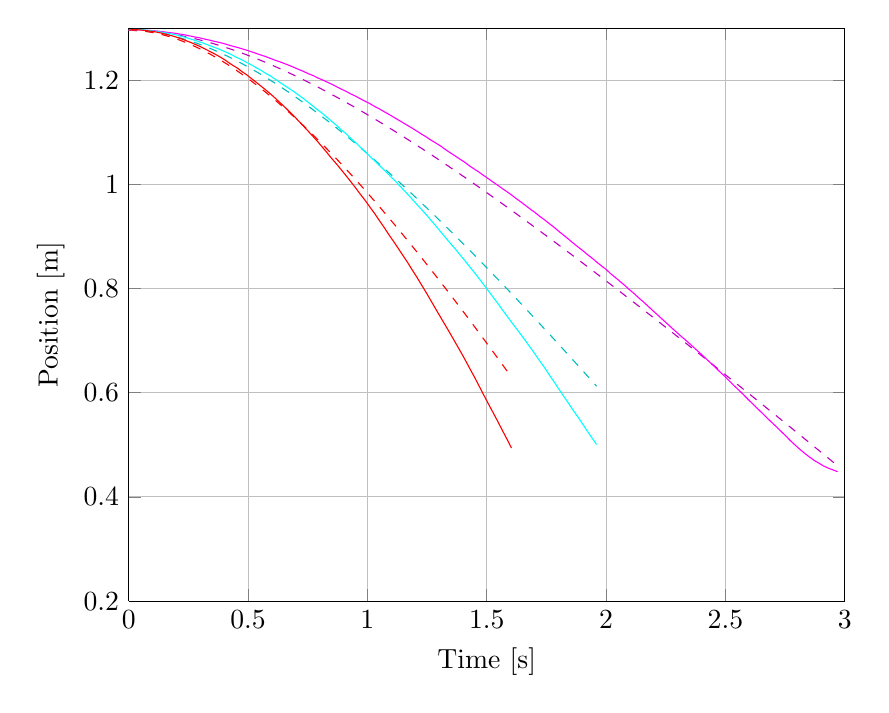
\begin{tikzpicture}

\begin{axis}[%
width=0.75\textwidth,
height=0.6\textwidth,
scale only axis,
separate axis lines,
every outer x axis line/.append style={black},
every x tick label/.append style={font=\color{black}},
xmin=0,
xmax=3,
xmajorgrids,
xlabel={Time [s]},
every outer y axis line/.append style={black},
every y tick label/.append style={font=\color{black}},
ymin=0.2,
ymax=1.3,
ymajorgrids,
ylabel={Position [m]},
axis background/.style={fill=white},
legend style={legend cell align=left,align=left,draw=black}
]
\addplot [color=mycolor1,dashed]
  table[row sep=crcr]{%
0	1.296\\
0.0198000198000198	1.29590934903503\\
0.0396000396000396	1.29564025462212\\
0.0594000594000594	1.29519692849233\\
0.0792000792000792	1.29458348296888\\
0.099000099000099	1.29380393331342\\
0.118800118800119	1.29286220001697\\
0.138600138600139	1.29176211103671\\
0.158400158400158	1.29050740398005\\
0.178200178200178	1.2891017282371\\
0.198000198000198	1.28754864706286\\
0.217800217800218	1.28585163961019\\
0.237600237600238	1.28401410291487\\
0.257400257400257	1.28203935383378\\
0.277200277200277	1.27993063093731\\
0.297000297000297	1.27769109635714\\
0.316800316800317	1.2753238375904\\
0.336600336600337	1.27283186926122\\
0.356400356400356	1.27021813484072\\
0.376200376200376	1.26748550832645\\
0.396000396000396	1.26463679588209\\
0.415800415800416	1.26167473743856\\
0.435600435600436	1.25860200825723\\
0.455400455400455	1.25542122045635\\
0.475200475200475	1.25213492450133\\
0.495000495000495	1.24874561065998\\
0.514800514800515	1.24525571042324\\
0.534600534600535	1.24166759789257\\
0.554400554400554	1.23798359113441\\
0.574200574200574	1.23420595350279\\
0.594000594000594	1.23033689493066\\
0.613800613800614	1.22637857319083\\
0.633600633600634	1.22233309512699\\
0.653400653400653	1.21820251785586\\
0.673200673200673	1.2139888499408\\
0.693000693000693	1.20969405253787\\
0.712800712800713	1.20532004051471\\
0.732600732600733	1.20086868354308\\
0.752400752400752	1.19634180716561\\
0.772200772200772	1.19174119383738\\
0.792000792000792	1.18706858394286\\
0.811800811800812	1.18232567678889\\
0.831600831600832	1.17751413157428\\
0.851400851400851	1.17263556833636\\
0.871200871200871	1.1676915688754\\
0.891000891000891	1.16268367765703\\
0.910800910800911	1.15761340269347\\
0.930600930600931	1.15248221640391\\
0.95040095040095	1.1472915564546\\
0.97020097020097	1.14204282657913\\
0.99000099000099	1.1367373973793\\
1.00980100980101	1.13137660710715\\
1.02960102960103	1.12596176242844\\
1.04940104940105	1.12049413916826\\
1.06920106920107	1.11497498303885\\
1.08900108900109	1.10940551035043\\
1.10880110880111	1.10378690870509\\
1.12860112860113	1.09812033767444\\
1.14840114840115	1.09240692946116\\
1.16820116820117	1.08664778954498\\
1.18800118800119	1.08084399731346\\
1.20780120780121	1.07499660667775\\
1.22760122760123	1.06910664667398\\
1.24740124740125	1.06317512205034\\
1.26720126720127	1.05720301384032\\
1.28700128700129	1.05119127992247\\
1.30680130680131	1.04514085556692\\
1.32660132660133	1.03905265396897\\
1.34640134640135	1.03292756677012\\
1.36620136620137	1.02676646456681\\
1.38600138600139	1.02057019740716\\
1.40580140580141	1.01433959527589\\
1.42560142560143	1.00807546856794\\
1.44540144540145	1.00177860855081\\
1.46520146520147	0.995449787816034\\
1.48500148500149	0.989089760719944\\
1.5048015048015	0.982699263814112\\
1.52460152460152	0.976279016265567\\
1.54440154440154	0.96982972026712\\
1.56420156420156	0.963352061437996\\
1.58400158400158	0.95684670921502\\
1.6038016038016	0.950314317234559\\
1.62360162360162	0.943755523705458\\
1.64340164340164	0.937170951773165\\
1.66320166320166	0.930561209875271\\
1.68300168300168	0.923926892088652\\
1.7028017028017	0.917268578468418\\
1.72260172260172	0.910586835378866\\
1.74240174240174	0.903882215816617\\
1.76220176220176	0.897155259726128\\
1.78200178200178	0.890406494307759\\
1.8018018018018	0.883636434318564\\
1.82160182160182	0.876845582365989\\
1.84140184140184	0.870034429194631\\
1.86120186120186	0.863203453966235\\
1.88100188100188	0.856353124533077\\
1.9008019008019	0.849483897704899\\
1.92060192060192	0.842596219509541\\
1.94040194040194	0.835690525447423\\
1.96020196020196	0.828767240740016\\
1.98000198000198	0.821826780572457\\
1.999801999802	0.814869550330429\\
2.01960201960202	0.807895945831455\\
2.03940203940204	0.800906353550732\\
2.05920205920206	0.793901150841633\\
2.07900207900208	0.786880706151007\\
2.0988020988021	0.779845379229396\\
2.11860211860212	0.772795521336291\\
2.13840213840214	0.76573147544054\\
2.15820215820216	0.758653576416033\\
2.17800217800218	0.751562151232762\\
2.1978021978022	0.744457519143374\\
2.21760221760222	0.73733999186532\\
2.23740223740224	0.730209873758705\\
2.25720225720226	0.723067461999943\\
2.27700227700228	0.715913046751308\\
2.2968022968023	0.708746911326487\\
2.31660231660232	0.701569332352224\\
2.33640233640234	0.694380579926151\\
2.35620235620236	0.687180917770891\\
2.37600237600238	0.679970603384524\\
2.3958023958024	0.672749888187504\\
2.41560241560242	0.665519017666106\\
2.43540243540244	0.658278231512489\\
2.45520245520246	0.651027763761449\\
2.47500247500248	0.643767842923953\\
2.49480249480249	0.636498692117511\\
2.51460251460251	0.629220529193478\\
2.53440253440253	0.621933566861349\\
2.55420255420255	0.614638012810119\\
2.57400257400257	0.607334069826782\\
2.59380259380259	0.600021935912027\\
2.61360261360261	0.592701804393212\\
2.63340263340263	0.585373864034666\\
2.65320265320265	0.578038299145385\\
2.67300267300267	0.570695289684192\\
2.69280269280269	0.563345011362414\\
2.71260271260271	0.555987635744128\\
2.73240273240273	0.548623330344057\\
2.75220275220275	0.541252258723134\\
2.77200277200277	0.53387458058183\\
2.79180279180279	0.526490451851268\\
2.81160281160281	0.519100024782187\\
2.83140283140283	0.511703448031815\\
2.85120285120285	0.504300866748679\\
2.87100287100287	0.496892422655422\\
2.89080289080289	0.489478254129664\\
2.91060291060291	0.482058496282951\\
2.93040293040293	0.474633281037845\\
2.95020295020295	0.46720273720319\\
2.97000297000297	0.459766990547605\\
};
%\addlegendentry{2A model};

\addplot [color=mycolor2,dashed]
  table[row sep=crcr]{%
0	1.296\\
0.0198000198000198	1.29586741475651\\
0.0396000396000396	1.29547383981473\\
0.0594000594000594	1.29482543521266\\
0.0792000792000792	1.29392821559532\\
0.099000099000099	1.29278805364643\\
0.118800118800119	1.29141068343902\\
0.138600138600139	1.28980170370706\\
0.158400158400158	1.28796658103976\\
0.178200178200178	1.28591065300057\\
0.198000198000198	1.28363913117252\\
0.217800217800218	1.28115710413167\\
0.237600237600238	1.2784695403504\\
0.257400257400257	1.27558129103221\\
0.277200277200277	1.27249709287948\\
0.297000297000297	1.2692215707961\\
0.316800316800317	1.26575924052614\\
0.336600336600337	1.26211451123032\\
0.356400356400356	1.25829168800167\\
0.376200376200376	1.25429497432178\\
0.396000396000396	1.25012847445912\\
0.415800415800416	1.2457961958107\\
0.435600435600436	1.2413020511885\\
0.455400455400455	1.23664986105193\\
0.475200475200475	1.2318433556876\\
0.495000495000495	1.2268861773376\\
0.514800514800515	1.22178188227761\\
0.534600534600535	1.21653394284593\\
0.554400554400554	1.2111457494246\\
0.574200574200574	1.20562061237382\\
0.594000594000594	1.19996176392061\\
0.613800613800614	1.19417236000304\\
0.633600633600634	1.18825548207077\\
0.653400653400653	1.18221413884324\\
0.673200673200673	1.17605126802623\\
0.693000693000693	1.16976973798801\\
0.712800712800713	1.16337234939587\\
0.732600732600733	1.15686183681405\\
0.752400752400752	1.15024087026393\\
0.772200772200772	1.14351205674742\\
0.792000792000792	1.13667794173438\\
0.811800811800812	1.12974101061494\\
0.831600831600832	1.12270369011752\\
0.851400851400851	1.11556834969346\\
0.871200871200871	1.10833730286881\\
0.891000891000891	1.10101280856441\\
0.910800910800911	1.09359707238465\\
0.930600930600931	1.08609224787591\\
0.95040095040095	1.07850043775525\\
0.97020097020097	1.07082369511012\\
0.99000099000099	1.06306402456975\\
1.00980100980101	1.0552233834489\\
1.02960102960103	1.04730368286457\\
1.04940104940105	1.03930678882643\\
1.06920106920107	1.03123452330144\\
1.08900108900109	1.0230886652534\\
1.10880110880111	1.0148709516579\\
1.12860112860113	1.00658307849339\\
1.14840114840115	0.998226701708807\\
1.16820116820117	0.989803438168349\\
1.18800118800119	0.981314866574018\\
1.20780120780121	0.972762528366322\\
1.22760122760123	0.964147928603752\\
1.24740124740125	0.955472536821489\\
1.26720126720127	0.946737787869852\\
1.28700128700129	0.937945082732944\\
1.30680130680131	0.929095789327989\\
1.32660132660133	0.920191243285794\\
1.34640134640135	0.911232748712794\\
1.36620136620137	0.902221578935108\\
1.38600138600139	0.893158977225035\\
1.40580140580141	0.884046157510405\\
1.42560142560143	0.874884305067182\\
1.44540144540145	0.865674577195723\\
1.46520146520147	0.856418103881078\\
1.48500148500149	0.8471159884377\\
1.5048015048015	0.837769308138941\\
1.52460152460152	0.828379114831693\\
1.54440154440154	0.818946435536512\\
1.56420156420156	0.809472273033593\\
1.58400158400158	0.799957606434899\\
1.6038016038016	0.790403391742795\\
1.62360162360162	0.780810562395497\\
1.64340164340164	0.771180029799642\\
1.66320166320166	0.761512683850292\\
1.68300168300168	0.751809393438664\\
1.7028017028017	0.742071006947872\\
1.72260172260172	0.732298352736978\\
1.74240174240174	0.722492239613606\\
1.76220176220176	0.71265345729541\\
1.78200178200178	0.702782776860645\\
1.8018018018018	0.69288095118811\\
1.82160182160182	0.682948715386697\\
1.84140184140184	0.672986787214811\\
1.86120186120186	0.662995867489884\\
1.88100188100188	0.652976640488228\\
1.9008019008019	0.64292977433545\\
1.92060192060192	0.632855921387647\\
1.94040194040194	0.622755718603611\\
1.96020196020196	0.612629787908243\\
};
%\addlegendentry{3A model};

\addplot [color=red,dashed]
  table[row sep=crcr]{%
0	1.296\\
0.0198000198000198	1.29582530593635\\
0.0396000396000396	1.29530673234462\\
0.0594000594000594	1.2944523956791\\
0.0792000792000792	1.2932702208246\\
0.099000099000099	1.29176794561795\\
0.118800118800119	1.28995312526285\\
0.138600138600139	1.28783313664046\\
0.158400158400158	1.2854151825183\\
0.178200178200178	1.28270629565979\\
0.198000198000198	1.27971334283676\\
0.217800217800218	1.27644302874733\\
0.237600237600238	1.27290189984121\\
0.257400257400257	1.26909634805484\\
0.277200277200277	1.26503261445828\\
0.297000297000297	1.26071679281604\\
0.316800316800317	1.25615483306387\\
0.336600336600337	1.25135254470354\\
0.356400356400356	1.24631560011739\\
0.376200376200376	1.24104953780475\\
0.396000396000396	1.2355597655419\\
0.415800415800416	1.2298515634675\\
0.435600435600436	1.22393008709514\\
0.455400455400455	1.21780037025485\\
0.475200475200475	1.21146732796513\\
0.495000495000495	1.20493575923721\\
0.514800514800515	1.19821034981314\\
0.534600534600535	1.19129567483923\\
0.554400554400554	1.18419620147639\\
0.574200574200574	1.17691629144886\\
0.594000594000594	1.16946020353285\\
0.613800613800614	1.16183209598628\\
0.633600633600634	1.15403602892138\\
0.653400653400653	1.14607596662111\\
0.673200673200673	1.13795577980101\\
0.693000693000693	1.12967924781762\\
0.712800712800713	1.12125006082484\\
0.732600732600733	1.11267182187927\\
0.752400752400752	1.10394804899598\\
0.772200772200772	1.09508217715572\\
0.792000792000792	1.08607756026471\\
0.811800811800812	1.07693747306823\\
0.831600831600832	1.06766511301905\\
0.851400851400851	1.05826360210168\\
0.871200871200871	1.04873598861366\\
0.891000891000891	1.03908524890477\\
0.910800910800911	1.02931428907513\\
0.930600930600931	1.01942594663335\\
0.95040095040095	1.0094229921154\\
0.97020097020097	0.999308130665403\\
0.99000099000099	0.989084003578997\\
1.00980100980101	0.978753189810359\\
1.02960102960103	0.968318207443613\\
1.04940104940105	0.95778151512953\\
1.06920106920107	0.947145513488305\\
1.08900108900109	0.936412546479231\\
1.10880110880111	0.925584902738044\\
1.12860112860113	0.914664816882706\\
1.14840114840115	0.90365447078836\\
1.16820116820117	0.892555994832204\\
1.18800118800119	0.881371469108974\\
1.20780120780121	0.870102924617741\\
1.22760122760123	0.858752344420699\\
1.24740124740125	0.847321664774596\\
1.26720126720127	0.835812776235471\\
1.28700128700129	0.824227524737304\\
1.30680130680131	0.812567712645218\\
1.32660132660133	0.800835099783813\\
1.34640134640135	0.789031404441236\\
1.36620136620137	0.777158304349552\\
1.38600138600139	0.765217437641969\\
1.40580140580141	0.753210403787474\\
1.42560142560143	0.741138764503416\\
1.44540144540145	0.729004044646536\\
1.46520146520147	0.716807733082978\\
1.48500148500149	0.704551283537757\\
1.5048015048015	0.692236115424187\\
1.52460152460152	0.67986361465372\\
1.54440154440154	0.667435134426685\\
1.56420156420156	0.654951996004348\\
1.58400158400158	0.642415489462762\\
1.6038016038016	0.62982687442882\\
};
%\addlegendentry{4A model};

\addplot [color=mycolor3,solid]
  table[row sep=crcr]{%
0	1.295853\\
0.0198000198000198	1.297393\\
0.0396000396000396	1.297008\\
0.0594000594000594	1.296623\\
0.0792000792000792	1.295853\\
0.099000099000099	1.295468\\
0.118800118800119	1.294698\\
0.138600138600139	1.293543\\
0.158400158400158	1.292388\\
0.178200178200178	1.291233\\
0.198000198000198	1.290078\\
0.217800217800218	1.288538\\
0.237600237600238	1.286998\\
0.257400257400257	1.285073\\
0.277200277200277	1.283148\\
0.297000297000297	1.281608\\
0.316800316800317	1.279298\\
0.336600336600337	1.277373\\
0.356400356400356	1.275063\\
0.376200376200376	1.273138\\
0.396000396000396	1.270828\\
0.415800415800416	1.268133\\
0.435600435600436	1.265438\\
0.455400455400455	1.263128\\
0.475200475200475	1.260433\\
0.495000495000495	1.257738\\
0.514800514800515	1.254658\\
0.534600534600535	1.251578\\
0.554400554400554	1.248498\\
0.574200574200574	1.245418\\
0.594000594000594	1.241953\\
0.613800613800614	1.238488\\
0.633600633600634	1.235408\\
0.653400653400653	1.231943\\
0.673200673200673	1.228478\\
0.693000693000693	1.224628\\
0.712800712800713	1.220778\\
0.732600732600733	1.216928\\
0.752400752400752	1.212693\\
0.772200772200772	1.209228\\
0.792000792000792	1.204608\\
0.811800811800812	1.200758\\
0.831600831600832	1.196523\\
0.851400851400851	1.192288\\
0.871200871200871	1.187668\\
0.891000891000891	1.183048\\
0.910800910800911	1.178813\\
0.930600930600931	1.173808\\
0.95040095040095	1.169573\\
0.97020097020097	1.164568\\
0.99000099000099	1.159948\\
1.00980100980101	1.155328\\
1.02960102960103	1.149938\\
1.04940104940105	1.145318\\
1.06920106920107	1.139928\\
1.08900108900109	1.134923\\
1.10880110880111	1.129533\\
1.12860112860113	1.124143\\
1.14840114840115	1.118753\\
1.16820116820117	1.113363\\
1.18800118800119	1.107973\\
1.20780120780121	1.102198\\
1.22760122760123	1.096423\\
1.24740124740125	1.091033\\
1.26720126720127	1.084873\\
1.28700128700129	1.079483\\
1.30680130680131	1.073708\\
1.32660132660133	1.067163\\
1.34640134640135	1.061003\\
1.36620136620137	1.055228\\
1.38600138600139	1.049068\\
1.40580140580141	1.043293\\
1.42560142560143	1.036363\\
1.44540144540145	1.030203\\
1.46520146520147	1.024428\\
1.48500148500149	1.017883\\
1.5048015048015	1.011723\\
1.52460152460152	1.005178\\
1.54440154440154	0.999018\\
1.56420156420156	0.992473\\
1.58400158400158	0.986313\\
1.6038016038016	0.979768\\
1.62360162360162	0.972838\\
1.64340164340164	0.966293\\
1.66320166320166	0.959363\\
1.68300168300168	0.952433\\
1.7028017028017	0.945888\\
1.72260172260172	0.938573\\
1.74240174240174	0.932028\\
1.76220176220176	0.924713\\
1.78200178200178	0.917783\\
1.8018018018018	0.910083\\
1.82160182160182	0.902768\\
1.84140184140184	0.895453\\
1.86120186120186	0.887753\\
1.88100188100188	0.880438\\
1.9008019008019	0.873508\\
1.92060192060192	0.865808\\
1.94040194040194	0.858878\\
1.96020196020196	0.851178\\
1.98000198000198	0.843863\\
1.999801999802	0.836933\\
2.01960201960202	0.828463\\
2.03940203940204	0.821148\\
2.05920205920206	0.813448\\
2.07900207900208	0.805748\\
2.0988020988021	0.797663\\
2.11860211860212	0.789963\\
2.13840213840214	0.781493\\
2.15820215820216	0.773793\\
2.17800217800218	0.765323\\
2.1978021978022	0.756853\\
2.21760221760222	0.748768\\
2.23740223740224	0.740298\\
2.25720225720226	0.732213\\
2.27700227700228	0.723743\\
2.2968022968023	0.715658\\
2.31660231660232	0.707573\\
2.33640233640234	0.699873\\
2.35620235620236	0.691788\\
2.37600237600238	0.683318\\
2.3958023958024	0.675233\\
2.41560241560242	0.666763\\
2.43540243540244	0.658293\\
2.45520245520246	0.649823\\
2.47500247500248	0.640968\\
2.49480249480249	0.632498\\
2.51460251460251	0.623643\\
2.53440253440253	0.614403\\
2.55420255420255	0.605933\\
2.57400257400257	0.597078\\
2.59380259380259	0.587838\\
2.61360261360261	0.578983\\
2.63340263340263	0.570128\\
2.65320265320265	0.561273\\
2.67300267300267	0.552418\\
2.69280269280269	0.543563\\
2.71260271260271	0.535093\\
2.73240273240273	0.526238\\
2.75220275220275	0.517383\\
2.77200277200277	0.508143\\
2.79180279180279	0.499673\\
2.81160281160281	0.491588\\
2.83140283140283	0.483888\\
2.85120285120285	0.476958\\
2.87100287100287	0.470413\\
2.89080289080289	0.465023\\
2.91060291060291	0.459633\\
2.93040293040293	0.455398\\
2.95020295020295	0.451933\\
2.97000297000297	0.448468\\
};
%\addlegendentry{2A samples};

\addplot [color=mycolor4,solid]
  table[row sep=crcr]{%
0	1.296448\\
0.0198000198000198	1.297603\\
0.0396000396000396	1.297603\\
0.0594000594000594	1.297218\\
0.0792000792000792	1.296063\\
0.099000099000099	1.294908\\
0.118800118800119	1.293753\\
0.138600138600139	1.292213\\
0.158400158400158	1.290673\\
0.178200178200178	1.289133\\
0.198000198000198	1.287208\\
0.217800217800218	1.284898\\
0.237600237600238	1.282588\\
0.257400257400257	1.279508\\
0.277200277200277	1.276813\\
0.297000297000297	1.273733\\
0.316800316800317	1.270653\\
0.336600336600337	1.267188\\
0.356400356400356	1.263723\\
0.376200376200376	1.260258\\
0.396000396000396	1.256408\\
0.415800415800416	1.252558\\
0.435600435600436	1.247938\\
0.455400455400455	1.243318\\
0.475200475200475	1.239083\\
0.495000495000495	1.234078\\
0.514800514800515	1.229458\\
0.534600534600535	1.224068\\
0.554400554400554	1.219063\\
0.574200574200574	1.213288\\
0.594000594000594	1.208283\\
0.613800613800614	1.202123\\
0.633600633600634	1.195963\\
0.653400653400653	1.189803\\
0.673200673200673	1.184028\\
0.693000693000693	1.177868\\
0.712800712800713	1.171323\\
0.732600732600733	1.164778\\
0.752400752400752	1.157463\\
0.772200772200772	1.150533\\
0.792000792000792	1.143218\\
0.811800811800812	1.136288\\
0.831600831600832	1.128588\\
0.851400851400851	1.120888\\
0.871200871200871	1.113188\\
0.891000891000891	1.104718\\
0.910800910800911	1.097403\\
0.930600930600931	1.088548\\
0.95040095040095	1.080463\\
0.97020097020097	1.071608\\
0.99000099000099	1.063523\\
1.00980100980101	1.054283\\
1.02960102960103	1.045813\\
1.04940104940105	1.036958\\
1.06920106920107	1.028103\\
1.08900108900109	1.019248\\
1.10880110880111	1.010008\\
1.12860112860113	1.000768\\
1.14840114840115	0.991143\\
1.16820116820117	0.981518\\
1.18800118800119	0.971508\\
1.20780120780121	0.961498\\
1.22760122760123	0.951488\\
1.24740124740125	0.941478\\
1.26720126720127	0.930698\\
1.28700128700129	0.920303\\
1.30680130680131	0.909138\\
1.32660132660133	0.898358\\
1.34640134640135	0.887578\\
1.36620136620137	0.877183\\
1.38600138600139	0.866018\\
1.40580140580141	0.855238\\
1.42560142560143	0.843688\\
1.44540144540145	0.832523\\
1.46520146520147	0.820973\\
1.48500148500149	0.809038\\
1.5048015048015	0.797103\\
1.52460152460152	0.784783\\
1.54440154440154	0.772848\\
1.56420156420156	0.760143\\
1.58400158400158	0.747823\\
1.6038016038016	0.735503\\
1.62360162360162	0.723568\\
1.64340164340164	0.711633\\
1.66320166320166	0.699313\\
1.68300168300168	0.686608\\
1.7028017028017	0.673903\\
1.72260172260172	0.660813\\
1.74240174240174	0.648108\\
1.76220176220176	0.634248\\
1.78200178200178	0.621158\\
1.8018018018018	0.607298\\
1.82160182160182	0.593823\\
1.84140184140184	0.580733\\
1.86120186120186	0.566873\\
1.88100188100188	0.554168\\
1.9008019008019	0.540693\\
1.92060192060192	0.526833\\
1.94040194040194	0.513743\\
1.96020196020196	0.500653\\
};
%\addlegendentry{3A samples};

\addplot [color=red,solid]
  table[row sep=crcr]{%
0	1.296223\\
0.0198000198000198	1.297378\\
0.0396000396000396	1.296993\\
0.0594000594000594	1.296223\\
0.0792000792000792	1.295068\\
0.099000099000099	1.293913\\
0.118800118800119	1.292373\\
0.138600138600139	1.290448\\
0.158400158400158	1.288138\\
0.178200178200178	1.285828\\
0.198000198000198	1.283133\\
0.217800217800218	1.280053\\
0.237600237600238	1.276588\\
0.257400257400257	1.273123\\
0.277200277200277	1.269273\\
0.297000297000297	1.265423\\
0.316800316800317	1.260803\\
0.336600336600337	1.256183\\
0.356400356400356	1.251563\\
0.376200376200376	1.246558\\
0.396000396000396	1.241168\\
0.415800415800416	1.235008\\
0.435600435600436	1.228848\\
0.455400455400455	1.223458\\
0.475200475200475	1.216528\\
0.495000495000495	1.210368\\
0.514800514800515	1.203053\\
0.534600534600535	1.196123\\
0.554400554400554	1.188808\\
0.574200574200574	1.181493\\
0.594000594000594	1.173793\\
0.613800613800614	1.165708\\
0.633600633600634	1.157238\\
0.653400653400653	1.148768\\
0.673200673200673	1.139913\\
0.693000693000693	1.131058\\
0.712800712800713	1.121433\\
0.732600732600733	1.111808\\
0.752400752400752	1.102183\\
0.772200772200772	1.092173\\
0.792000792000792	1.082163\\
0.811800811800812	1.071383\\
0.831600831600832	1.060603\\
0.851400851400851	1.049438\\
0.871200871200871	1.039043\\
0.891000891000891	1.027878\\
0.910800910800911	1.016713\\
0.930600930600931	1.005163\\
0.95040095040095	0.993613\\
0.97020097020097	0.981293\\
0.99000099000099	0.969743\\
1.00980100980101	0.957038\\
1.02960102960103	0.944718\\
1.04940104940105	0.931243\\
1.06920106920107	0.918153\\
1.08900108900109	0.904293\\
1.10880110880111	0.891203\\
1.12860112860113	0.877728\\
1.14840114840115	0.863868\\
1.16820116820117	0.850393\\
1.18800118800119	0.835763\\
1.20780120780121	0.821518\\
1.22760122760123	0.806503\\
1.24740124740125	0.791488\\
1.26720126720127	0.776088\\
1.28700128700129	0.760303\\
1.30680130680131	0.744903\\
1.32660132660133	0.729503\\
1.34640134640135	0.714103\\
1.36620136620137	0.698318\\
1.38600138600139	0.682533\\
1.40580140580141	0.666363\\
1.42560142560143	0.649423\\
1.44540144540145	0.632868\\
1.46520146520147	0.615543\\
1.48500148500149	0.597833\\
1.5048015048015	0.580508\\
1.52460152460152	0.563568\\
1.54440154440154	0.546628\\
1.56420156420156	0.528918\\
1.58400158400158	0.511593\\
1.6038016038016	0.493883\\
};
%\addlegendentry{4A samples};

\end{axis}

\begin{axis}[%
width=0.85\textwidth,
height=0.6\textwidth,
at={(1.85in,0.746in)},
scale only axis,
every outer x axis line/.append style={black},
every x tick label/.append style={font=\color{black}},
xmin=0,
xmax=1,
xlabel={Time [s]},
every outer y axis line/.append style={black},
every y tick label/.append style={font=\color{black}},
ymin=0,
ymax=1,
ylabel={Position [m]},
hide axis,
axis x line*=bottom,
axis y line*=left
]
\end{axis}
\end{tikzpicture}%
              \end{figure}}	     	
    \end{itemize}           
  \end{minipage}
\end{frame} 
%%%%%%%%%%%%%%%%
